\chapter{Trasmissione del Moto mediante Ruote Dentate}\index{ruote!dentate}\label{cap_ruote_ev}

\section{Le Ruote di Frizione}
\noindent Credo che a ben pochi lettori sfugga, almeno da un punto di vista
meramente visivo, cosa sia una {\em ruota dentata}.

\begin{wrapfigure}{r}{0.48\textwidth}
      \begin{center}
      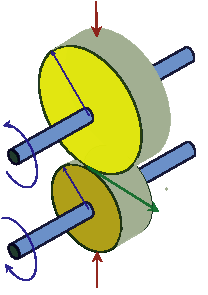
\includegraphics[width=0.43\textwidth]{part2/ruote/FIG/f22.pdf}
     \end{center}
\begin{picture}(0,0)(-63,1)
\scriptsize{
\put(21,235){$\bm F$}
\put(-2,190){$r_1$}
\put(4,108){$r_2$}
\put(-55,159){$\omega_1$}
\put(-55,40){$\omega_2$}
\put(21,40){$\bm F$}
\put(65,89){$v_1=v_2$}
}
\end{picture}
        \caption{\em Ruote di frizione.}
     \label{fig:f22}
\end{wrapfigure}

\noindent Le ruote dentate sono comparse alla maggior parte di noi in contesti
eterogenei che vanno dai giochi per bambini agli elettrodomestici, ad alcuni
strumenti da cartoleria, senza parlare dell'emblema della Repubblica Italiana.
Qualche privilegiato ha potuto vedere le ruote dentate impiegate nella
meccanica delle automobili e dei motoveicoli. Tutti possono agevolmente 
immaginare (qualora non ne avessimo contezza diretta) il relativo ingranamento di una ruota dentata con una sua simile.  

\noindent Lasciamo per il momento da parte la caratteristica fondamentale di queste
ruote, che si manifesta tramite una serie di sporgenze opportune, chiamate denti.
Fissiamo invece 
le idee su due cilindri, che presentino raggi adeguati ai nostri
scopi, pensando di calettarli sui
rispettivi alberi, paralleli e liberi di ruotare attorno ai propri assi.
Possiamo fare in modo che le superfici cilindriche siano tra loro
a contatto e che tale contatto sia mantenuto da una data forza $\bm F$.
La figura \ref{fig:f22} rappresenta i due cilindri coi rispettivi alberi.
Ipotizzando che il moto relativo di una ruota rispetto all'altra sia di puro
rotolamento, possiamo affermare che le velocit\`a angolari dei due alberi
dovranno essere tali da produrre velocit\`a periferiche uguali
tra loro sulle due ruote.
Cio\`e dovr\`a valere $v_1=\omega_1 r_1 = v_2 = \omega_2 r_2$, 
relazione che permette di ricavare subito il {\em rapporto di trasmissione}\index{rapporto di trasmissione} della coppia di 
{\em ruote di frizione}\index{ruote!di frizione},
\begin{equation}
\tau={\omega_1\over{\omega_2}}=
{{r_2}\over{r_1}}\,.
\label{eq:tau}
\end{equation}
\noindent I due alberi ruotano pertanto con velocit\`a angolari differenti tra
loro e in strettissima relazione coi raggi delle due ruote che trasmettono
il moto. Nonostante le ruote di frizione siano realmente esistite nel
mondo della meccanica\footnote
{
Un curioso esempio di applicazione: il FERMIAC era un calcolatore analogico basato su ruote di frizione.
}, e si trovino ancora in applicazioni dove le
potenze in gioco sono sia molto grandi sia molto piccole, credo che il
loro pi\`u grave inconveniente potenziale, cio\`e
la possibilit\`a che il loro moto relativo di puro rotolamento venga
contaminato dallo strisciamento, sia evidente anche ad occhi non
particolarmente esperti. Non riteniamo opportuno chiarire
in questa sede il  meccanismo dell'attrito (in prevalenza statico)
necessario a trasmettere correttamente il moto in determinate condizioni,
n\'e illustreremo come possono essere realizzate, nella pratica, le coppie
di ruote di frizione, che tuttavia si fabbricano ancora, come
abbiamo appena affermato, anche
nel contesto di rilevanti potenze da trasmettere.
In questo luogo, ci basta osservare che
la trasmissione corretta del moto, tramite questi dispositivi,
\`e condizionata dal valore della forza $\bm F$ mediante la quale
le ruote sono costrette a mantenere il contatto tra loro.
In cascata, il valore efficace di tale forza \`e subordinato
al coefficiente di attrito tra le due superfici, a sua volta soggetto
a variazioni non leggere del suo valore,
a causa dell'usura e delle condizioni, probabilmente mutevoli, di
lubrificazione delle ruote stesse.
La garanzia del rapporto di trasmissione teorico, derivante dal rapporto tra i
diametri delle ruote, \`e perci\`o negata dai probabili scorrimenti
tra le due primitive nel punto di contatto.


\section{Percorso Intuitivo verso le Ruote Dentate} \label{percorso-ruote}

\noindent Riprendendo il filo dal precedente paragrafo,
siamo naturalmente tentati di impedire lo slittamento della trasmissione
ponendo su una delle ruote
alcune sporgenze e ricavando sulla seconda ruota degli incavi, tali da accogliere
le suddette sporgenze.
Inizieremo a breve un cammino che possiamo definire {\em induttivo}, a valle
del quale riteniamo che la soluzione,
adottata nella pratica come {\em standard} per la creazione delle
ruote dentate, dovrebbe essere ricevuta senza perplessit\`a. 
Premettiamo per\`o alcune considerazioni che riguardano il taglio che abbiamo
desiderato dare all'esposizione del presente argomento.
Le ruote dentate rappresentano nella meccanica gli organi maggiormente
diffusi nell'ambito della trasmissione e della trasformazione del moto, in
generale rotatorio. Si comprende perci\`o facilmente la loro
centralit\`a
in quasi tutte le applicazioni industriali. Crediamo di non esagerare dicendo
che esse rappresentano l'oggetto simbolo della meccanica e del funzionamento
delle macchine.
Pertanto, anche se nella Meccanica Applicata alle Macchine esse godono di una
posizione privilegiata, il loro studio si incontra anche in altre discipline
dell'ingegneria: nel Disegno di Macchine, nella Costruzione di Macchine e nella
Tecnologia Meccanica. Naturalmente, ci\`o accade anche per altri argomenti
di particolare interesse nella nostra 
materia. Tuttavia, ci \`e sembrato di notare 
che le ruote dentate vengano esposte anche altrove
con molta attenzione persino ai loro aspetti cinematici
e geometrici che ne determinano un
buono o cattivo funzionamento: cosa strana, questa, perch\'e l'aspetto
cinematico legato all'ingranamento \`e un argomento piuttosto intricato ma,
forse per questo, si ritiene che non sia mai chiarito a sufficienza.
Cercheremo, come sempre in queste note,
di rimanere circoscritti ai soli aspetti cinematico-geometrici
di questi dispositivi, divagando solamente quando qualche altra loro
caratteristica
(resistenza, facilit\`a di realizzazione e possibilit\`a di impiego) 
sar\`a determinante nel condizionarne la forma. Per tale motivo, questo volume,
che tratta esclusivamente la cinematica, non include
una porzione massiccia di particolarit\`a e di connotazioni delle
ruote dentate, alcune anche molto comuni, altre maggiormente 
tecniche, fondamentali per il loro
effettivo impiego. Un esempio che crediamo significativo:
non tratteremo le ruote con dentatura elicoidale, di grande importanza
nella pratica ma cinematicamente non dissimili dalle loro sorelle
a denti diritti.
Assicuriamo coloro i quali volessero
investigare le ruote dentate nei loro
aspetti pi\`u profondi e nella loro variet\`a di tipologie e applicazioni
che testi molto pi\`u completi, autorevoli e dettagliati
del nostro non mancano. A nostro parere, ad esempio,
questo argomento \`e esposto in modo rigoroso ed esaustivo in
\cite{pellicano}; indichiamo anche un manuale, a livello di scuola superiore,
che riporta un numero notevole di esempi utili per 
il progettista: \cite{punzi}. La ``Bibbia'' in questo campo, ad oggi, rimane \cite{henriot}.

\noindent Come abbiamo gi\`a accennato, riteniamo che
da un punto di vista didattico
sia efficace seguire una sorta di sentiero, percorrendo il quale
saremo costretti ad ammettere
che la possibilit\`a di proseguire sia condizionata dall'accettazione
di alcuni ``precetti'', pi\`u o meno tassativi, dettati da particolari
e stringenti circostanze.
Lungo tale percorso incontreremo pertanto
precetti forti e precetti deboli, e queste due qualit\`a saranno indicate tra
parentesi. Un precetto forte non potr\`a ammettere eccezioni, mentre uno
debole potr\`a essere in qualche caso disatteso, e quando lo sar\`a,
cercheremo di chiarire il perch\'e.
Inizieremo il nostro cammino dalle
ruote di frizione introdotte poco sopra, proponendo
un tentativo per la loro modifica,
in modo da assicurarle dal pericolo di
scorrere l'una sull'altra.
L'esperimento (mentale) che si pu\`o condurre \`e quello
di dotare una delle due ruote di alcune sporgenze che, inserendosi
in opportuni incavi ricavati sull'altra ruota, riescano a trasmettere
la componente tangenziale della forza, che le due ruote si scambiano,
senza basarsi sul fenomeno dell'attrito. Potremmo 
pensare alla ruota che deve essere incavata come fatta di plastilina
o di un qualunque materiale plastico e tenero, che possa poi indurire.
In questa materia plastica la ruota recante le asperit\`a potr\`a
pertanto operare un'azione
di incisione. Questo procedimento di taglio deve essere
condotto pensando che le due circonferenze delle ruote di frizione, 
che chiameremo {\em circonferenze primitive}\index{circonferenza!primitiva},
rotolino l'una sull'altra senza strisciare. Si intuisce che,
i due profili, quello della ruota creatrice
unitamente a quello tagliato nella plastilina,
una volta indurito, saranno
in grado di trasmettere il moto allo stesso modo delle due primitive
rotolanti, cio\`e con rapporto di trasmissione
costante.

\begin{figure}[hbt]
\begin{center}
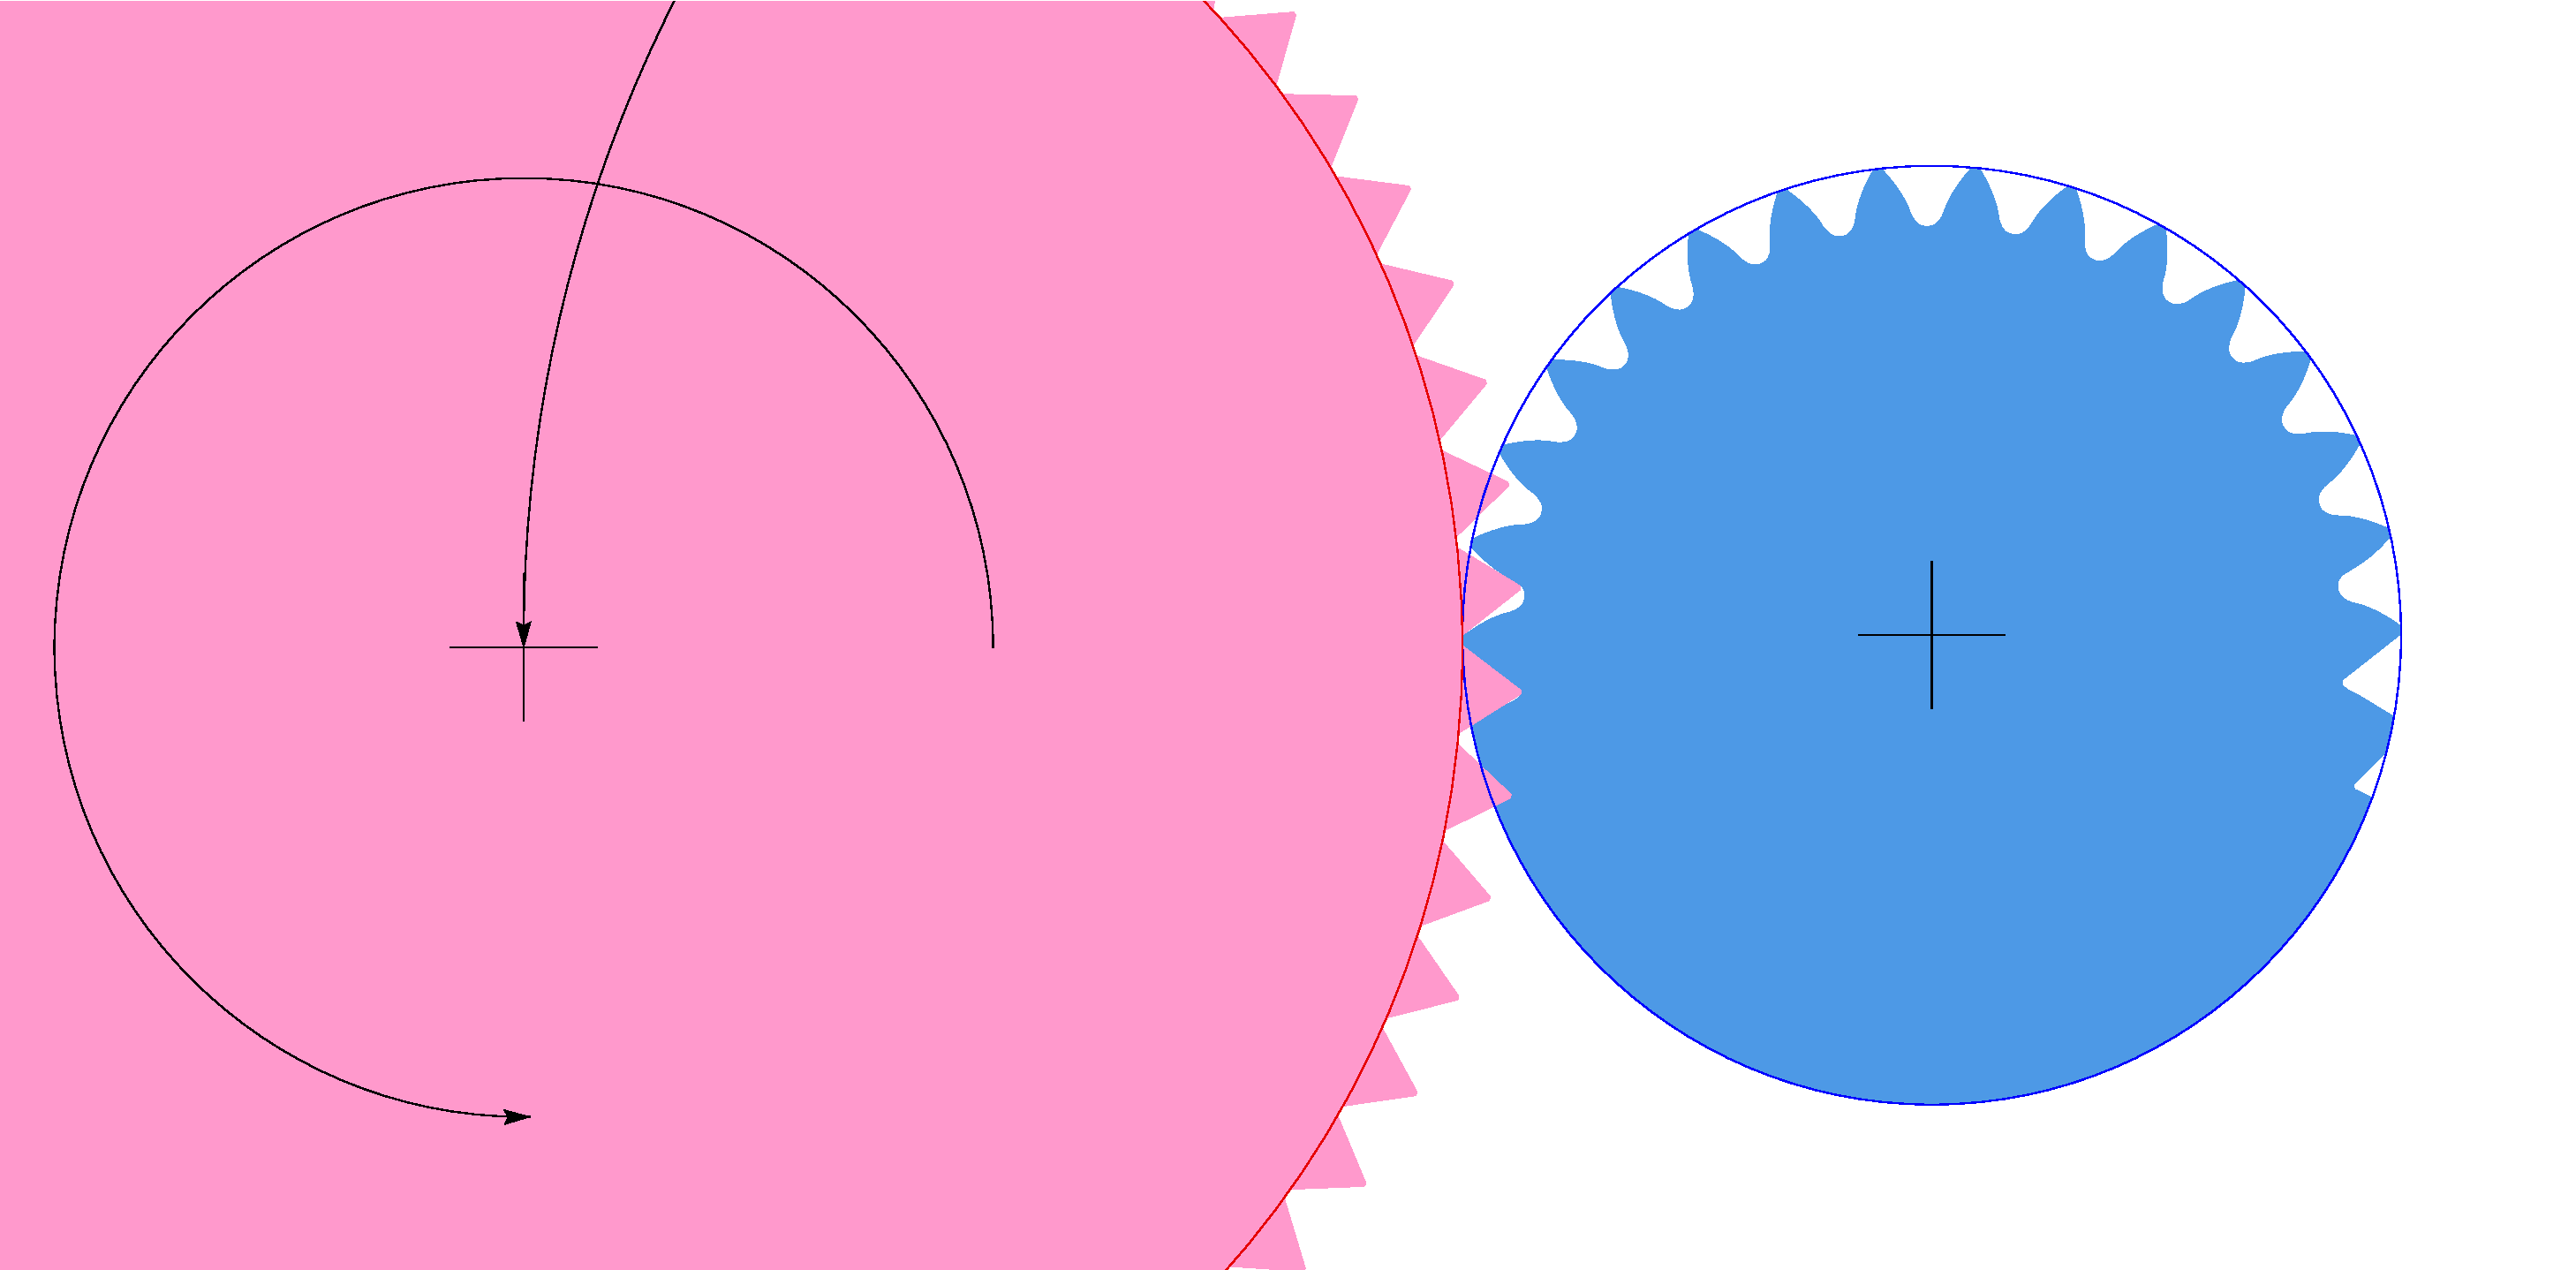
\includegraphics[width=0.8\textwidth]{part2/ruote/FIG/ruote/belbon.pdf}
\end{center}
\begin{picture}(0,0)(130,0)
\scriptsize{
\put(229,101){$\alpha=180^{\circ}$}
\put(214,34){$\beta=270^{\circ}$}
\put(350,63){ruota 1 tagliata}
\put(250,50){ruota 2 creatrice}
}
\end{picture}
\vskip -7mm
      \caption{\em Dentatura ingenua, 
ottenuta mediante l'applicazione di sporgenze triangolari alla ruota di
sinistra. $\alpha$ \`e l'arco di dentatura della ruota azzurra,
$\beta$ la rotazione della ruota rosa.}
 \label{fig:belbon}
\end{figure}

\noindent La figura \ref{fig:belbon} rappresenta una ruota creatrice,
di colore rosa, recante delle
sporgenze a triangolo isoscele all'esterno della propria circonferenza primitiva, 
esterne cio\`e alla circonferenza della ruota di frizione.
Tale ruota, di colore rosa,``intaglia'', tramite le sue sporgenze,
i denti sulla ruota azzurra.
Il primo precetto che emerge (forte) esige
un lieto fine per la dentatura della ruota tagliata (azzurra).
In altre parole, risulta fondamentale che,
una volta completato il taglio sui $360^{\circ}$ di tale ruota,
essa presenti
un numero intero di denti. Riteniamo inutile commentare questa
indicazione. Aggiungiamo solamente che, se il numero
di denti sulla ruota azzurra risultasse frazionario,
la sua dentatura verrebbe
distrutta da ulteriori passaggi della ruota creatrice.
Allo scopo di prevenire il citato inconveniente e di ottemperare
a questo precetto, la progettazione delle 
ruote dentate si basa principalmente sul loro numero di denti e
non sui loro diametri,
rendendo cos\`i di fatto impossibili rapporti di trasmissione rappresentati
da frazioni stravaganti o, peggio, da numeri irrazionali. Per fortuna
il mondo della tecnica non richiede tali prestazioni!
Scelta quindi una coppia di numeri di denti che meglio si adatta al
rapporto di trasmissione che vogliamo realizzare, giungeremo poi
alla reale dimensione delle ruote introducendo un numero dimensionale
che chiamiamo {\em modulo}\index{modulo}, $m$, misurato in millimetri,
legato al diametro della ruota nel modo seguente: $D= z\, m$, con $z$
numero di denti della ruota e $D$  diametro primitivo (quello
della corrispondente ruota di frizione). Va da s\'e che il
{\em passo}\index{passo}, cio\`e
la misura dell'arco di circonferenza primitiva che separa i due fianchi
attigui e omologhi, sinistri o destri, di due denti vale $p=\pi m$.

\noindent Un secondo precetto (debole) \`e la richiesta, per le asperit\`a del
creatore, di simmetria speculare rispetto a un raggio.
In effetti, le nostre sporgenze sono triangoli isosceli e ci\`o permette di
ottenere condizioni geometriche pari nei due sensi di marcia. Questa
\`e una restrizione che viene, in particolarissimi e rari casi, disattesa.
Ci accorgiamo per\`o, a questo punto, che la ruota azzurra ora
tagliata non potr\`a facilmente generare altri {\em partner}.
La via pi\`u breve per renderci conto di ci\`o consiste nel tentativo
di tagliare una gemella della ruota azzurra
(magari con ugual numero di denti)
utilizzando lei stessa come
creatore.
Purtroppo, trovandosi in questo caso le sporgenze della ruota creatrice
(la azzurra di figura
\ref{fig:belbon}) al di sotto della primitiva,
essa non sar\`a in grado di incidere alcunch\'e sul disco grezzo, lasciandoci
perplessi circa la nostra scelta.
Tuttavia ci accorgiamo che tagliare la {\em partner} della ruota azzurra di
figura \ref{fig:belbon}
tramite lei stessa non \`e il solo metodo che
abbiamo a disposizione.
\begin{figure}[hbt]
\begin{center}
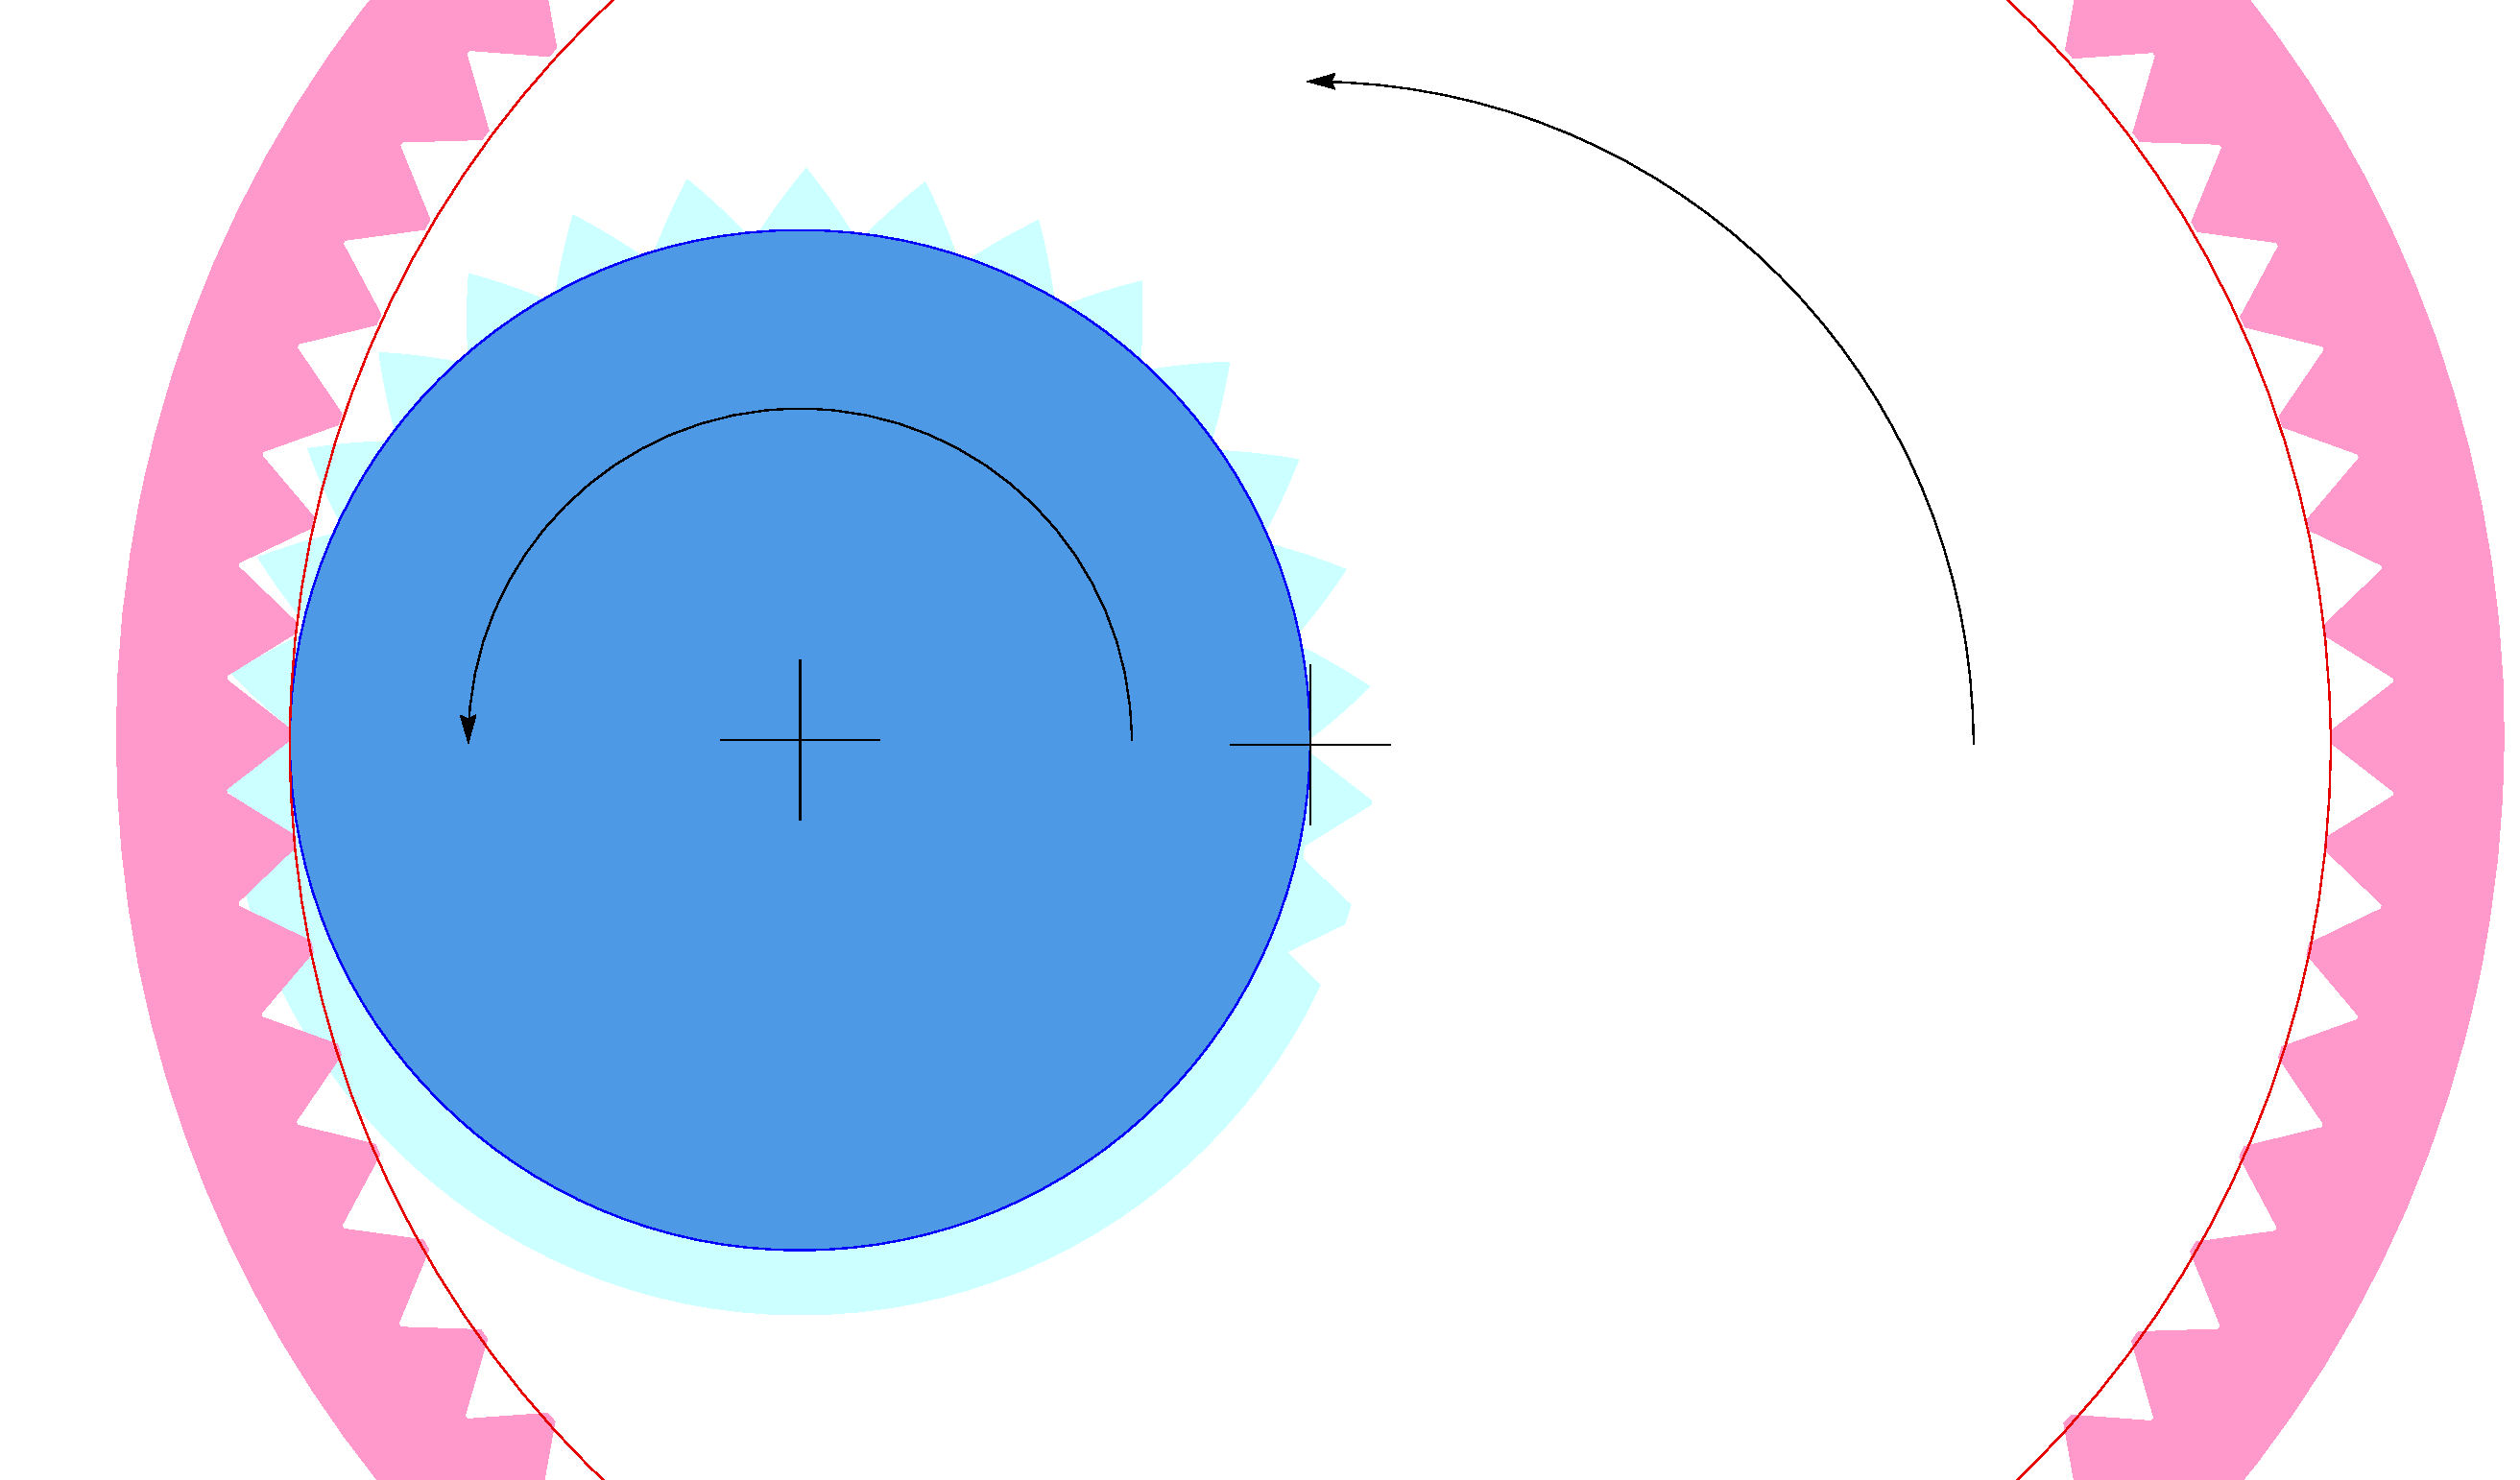
\includegraphics[width=0.72\textwidth]{part2/ruote/FIG/ruote/belbon_interno.pdf}
\end{center}
\begin{picture}(0,0)(0,0)
\scriptsize{
\put(96,95){$\alpha=180^{\circ}$}
\put(175,174){$\beta=90^{\circ}$}
\put(106,62){ruota 1 tagliata}
\put(300,50){ruota 2 creatrice}
}
\end{picture}
\vskip -7mm
      \caption{\em 
Tentativo di dentatura complementare con dentiera a curvatura negativa. La dentatura risulta impossibile.
}
 \label{fig:belbon_interno}
\end{figure}
La ruota rosa (creatrice) di figura \ref{fig:belbon}
possiede un utensile ``duale'' che consiste nella
stessa ruota con curvatura opposta.
Questa inversione, necessaria, della curvatura del creatore non pu\`o
essere chiarita a dovere in questo luogo. Rassicuriamo il lettore che, nel
paragrafo dove si tratta l'ottenimento dei profili coniugati di assortimento,
ci\`o risulter\`a perfettamente illustrato. Qui basta dire che questo
utensile ``duale'', rappresentato in rosa in figura \ref{fig:belbon_interno},
sarebbe perfettamente in grado,
come si intuisce dal suo aspetto, di creare la ruota 
rosa di figura \ref{fig:belbon}.
Ma anche in questo caso, rappresentato appunto
in figura \ref{fig:belbon_interno},
si nota che la ruota creatrice non trova materiale da incidere sullo
stesso disco grezzo dalla quale abbiamo ottenuto la ruota azzurra.
In tale figura viene riportato, con colore tenue, il sovra-metallo necessario
per potere tagliare questa benedetta {\em partner}. Ma \`e chiaro che l'obbligo
di impiegare dischi grezzi
differenti prelude alla necessit\`a di tollerare l'esistenza di
due famiglie di ruote, i membri di una delle quali, probabilmente,
ingraneranno coi membri dell'altra.
Si giunge cos\`i a un terzo precetto (forte) che \`e quello
di potere creare ruote, magari di due generi diversi che chiamiamo
a) e b), in
cui tutte le ruote appartenenti alla famiglia a) possano ingranare con quelle
appartenenti alla famiglia b)\footnote{
Questo requisito minimo per quanto riguarda l'assortibilit\`a delle ruote
dentate viene quasi sempre abbondantemente rispettato, anzi, nelle dentature
ad evolvente, come vedremo, le due famiglie si riducono a una.
}.
L'idea che ci viene in mente per ottemperare a tale precetto, 
quello cio\`e di far s\`i che esistano due famiglie di ruote,
che chiameremo di {\em assortimento}\index{ruote!di assortimento}
 e che siano simmetriche dal punto di vista 
del sovra-metallo che il disco grezzo deve presentare all'esterno
della circonferenza primitiva, consta nel creare sulla dentatrice
un profilo
che stia a cavallo della sua stessa primitiva.
\begin{figure}[hbt]
\begin{center}
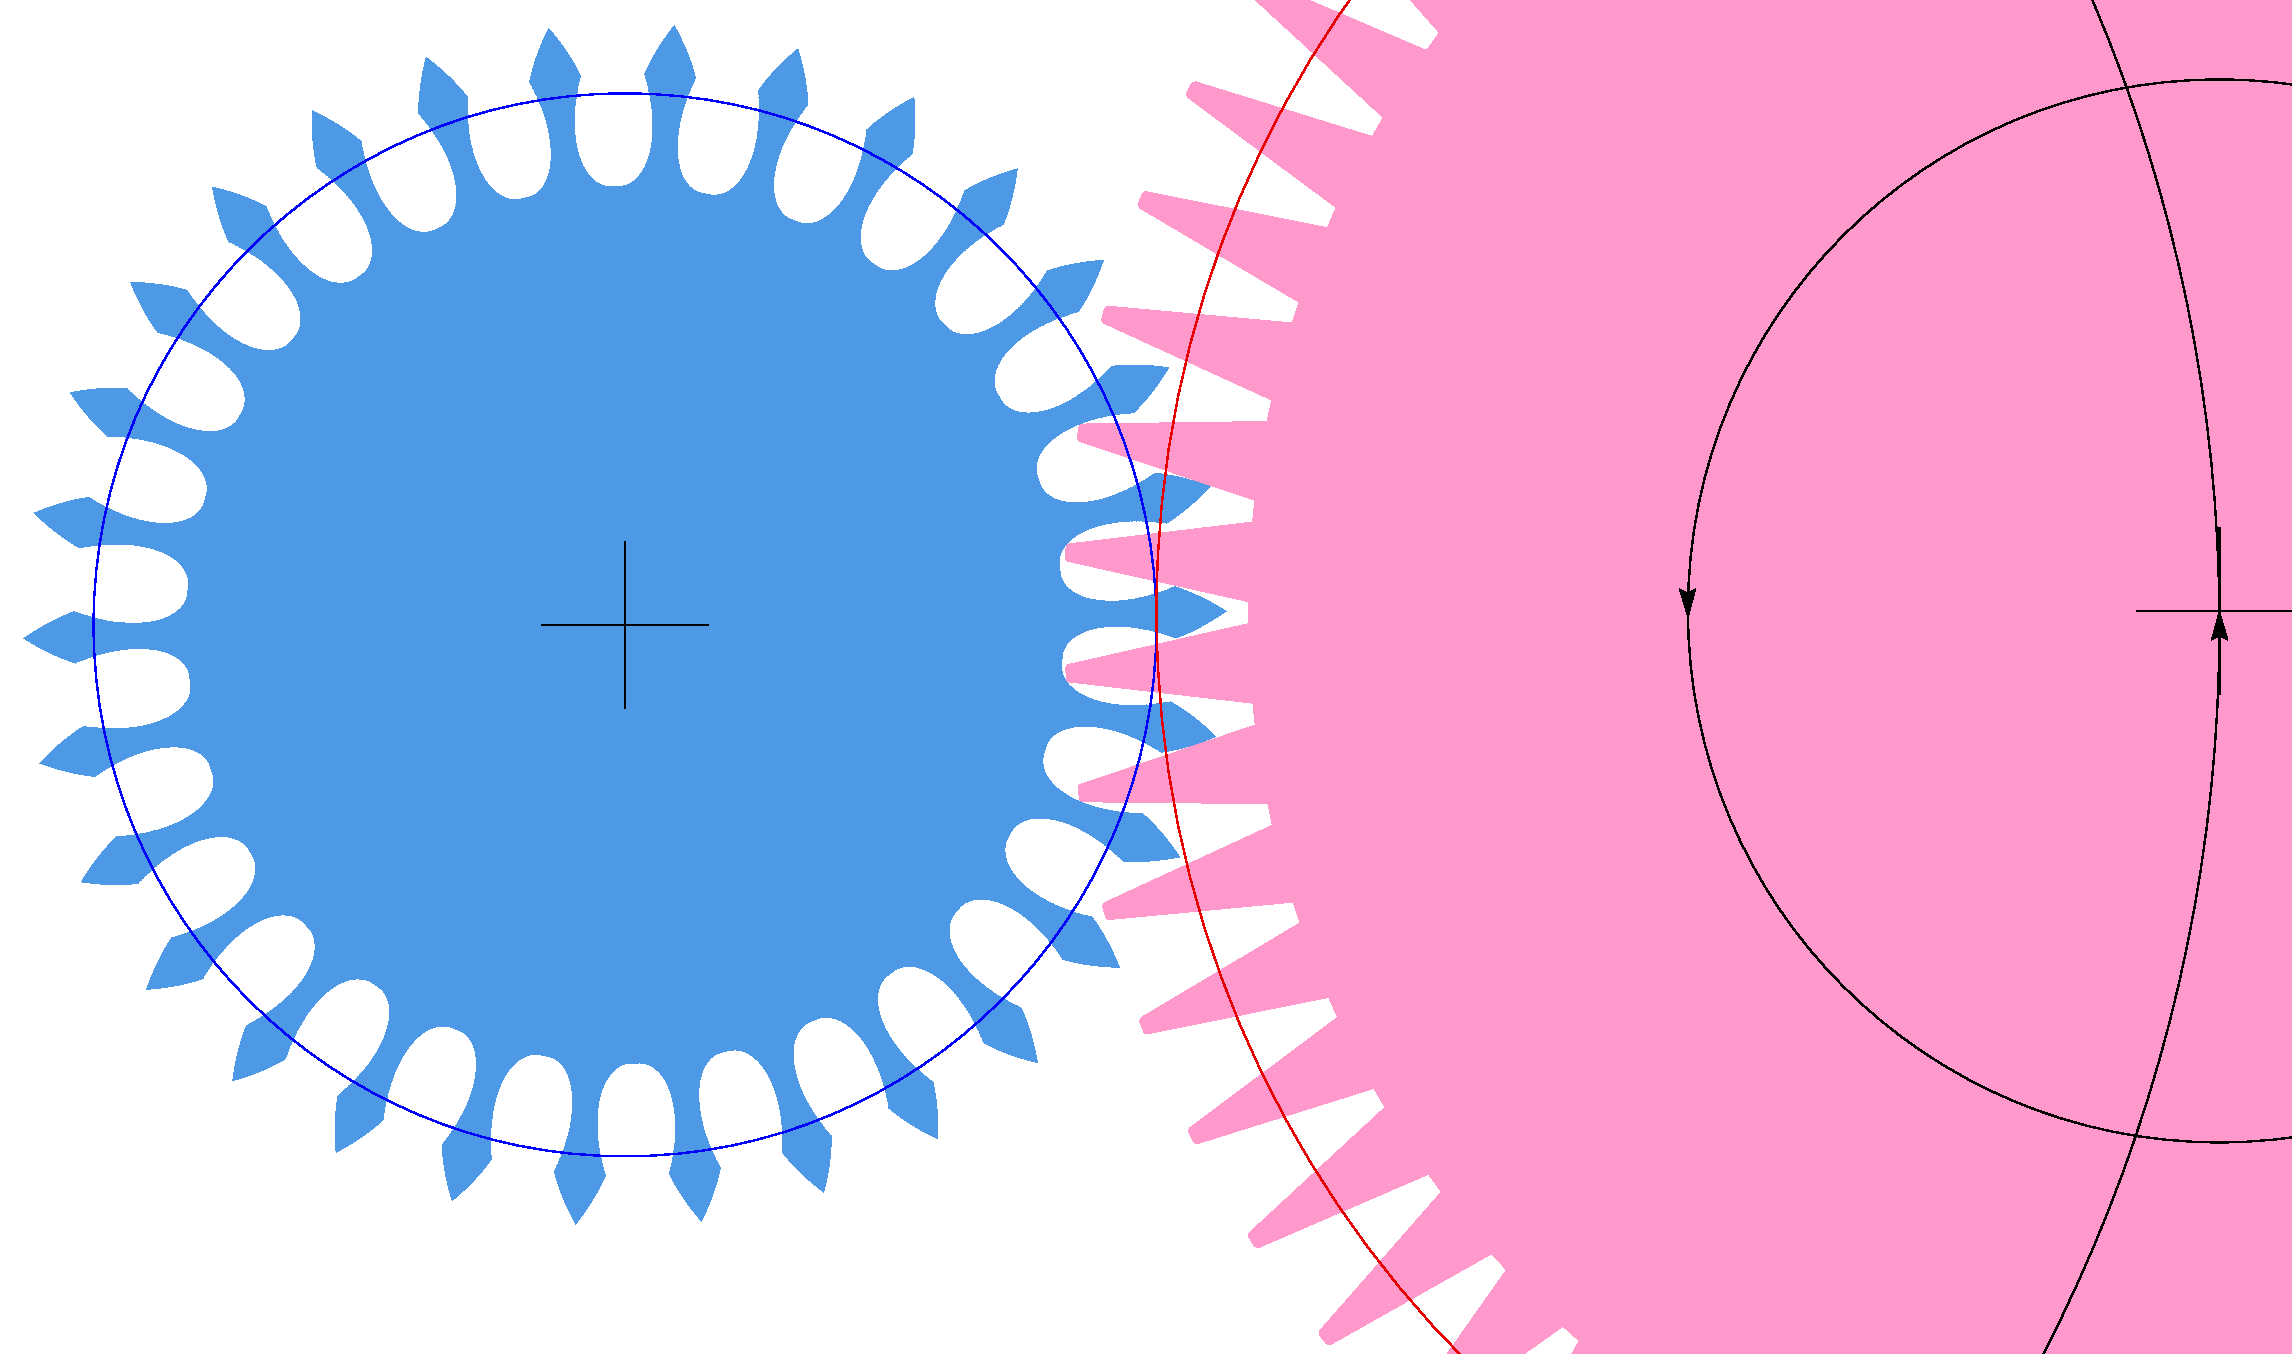
\includegraphics[width=0.85\textwidth]{part2/ruote/FIG/ruote/squalo.pdf}
\end{center}
\begin{picture}(0,0)(0,0)
\scriptsize{
\put(290,115){$\alpha=360^{\circ}$}
\put(220,133){$\beta=540^{\circ}$}
\put(85,145){famiglia a)}
\put(85,80){ruota 1 tagliata}
\put(230,50){ruota 2 creatrice}
}
\end{picture}
\vskip -7mm
      \caption{
\em Dentatura ottenuta da sporgenze a ``dente di squalo''. I denti creatori
misurano, sulla primitiva, quanto gli spazi vuoti.
I numeri di denti valgono $z_1=30$ e $z_2=60$.
}
 \label{fig:squalo}
\end{figure}
Il secondo tentativo,
rappresentato in figura \ref{fig:squalo}, mostra una dentatrice a ``denti di 
pescecane'' che taglia la ruota azzurra.
La dentatura \`e in questo caso presentata
completa, sottolineando cos\`i il rispetto del precetto che
impone numeri
di denti interi sulle due ruote, $z_1$ e $z_2$. Anche se confessiamo
 che le stesse figure
\ref{fig:belbon} e \ref{fig:belbon_interno} presenterebbero, sia
sulla ruota creatrice sia su quella tagliata,
un numero intero di denti
qualora tali ruote fossero rappresentate complete:
 non abbiamo avuto il coraggio di scrivere
una procedura che ammettesse le frazioni di dente.
\begin{figure}[hbt]
\begin{center}
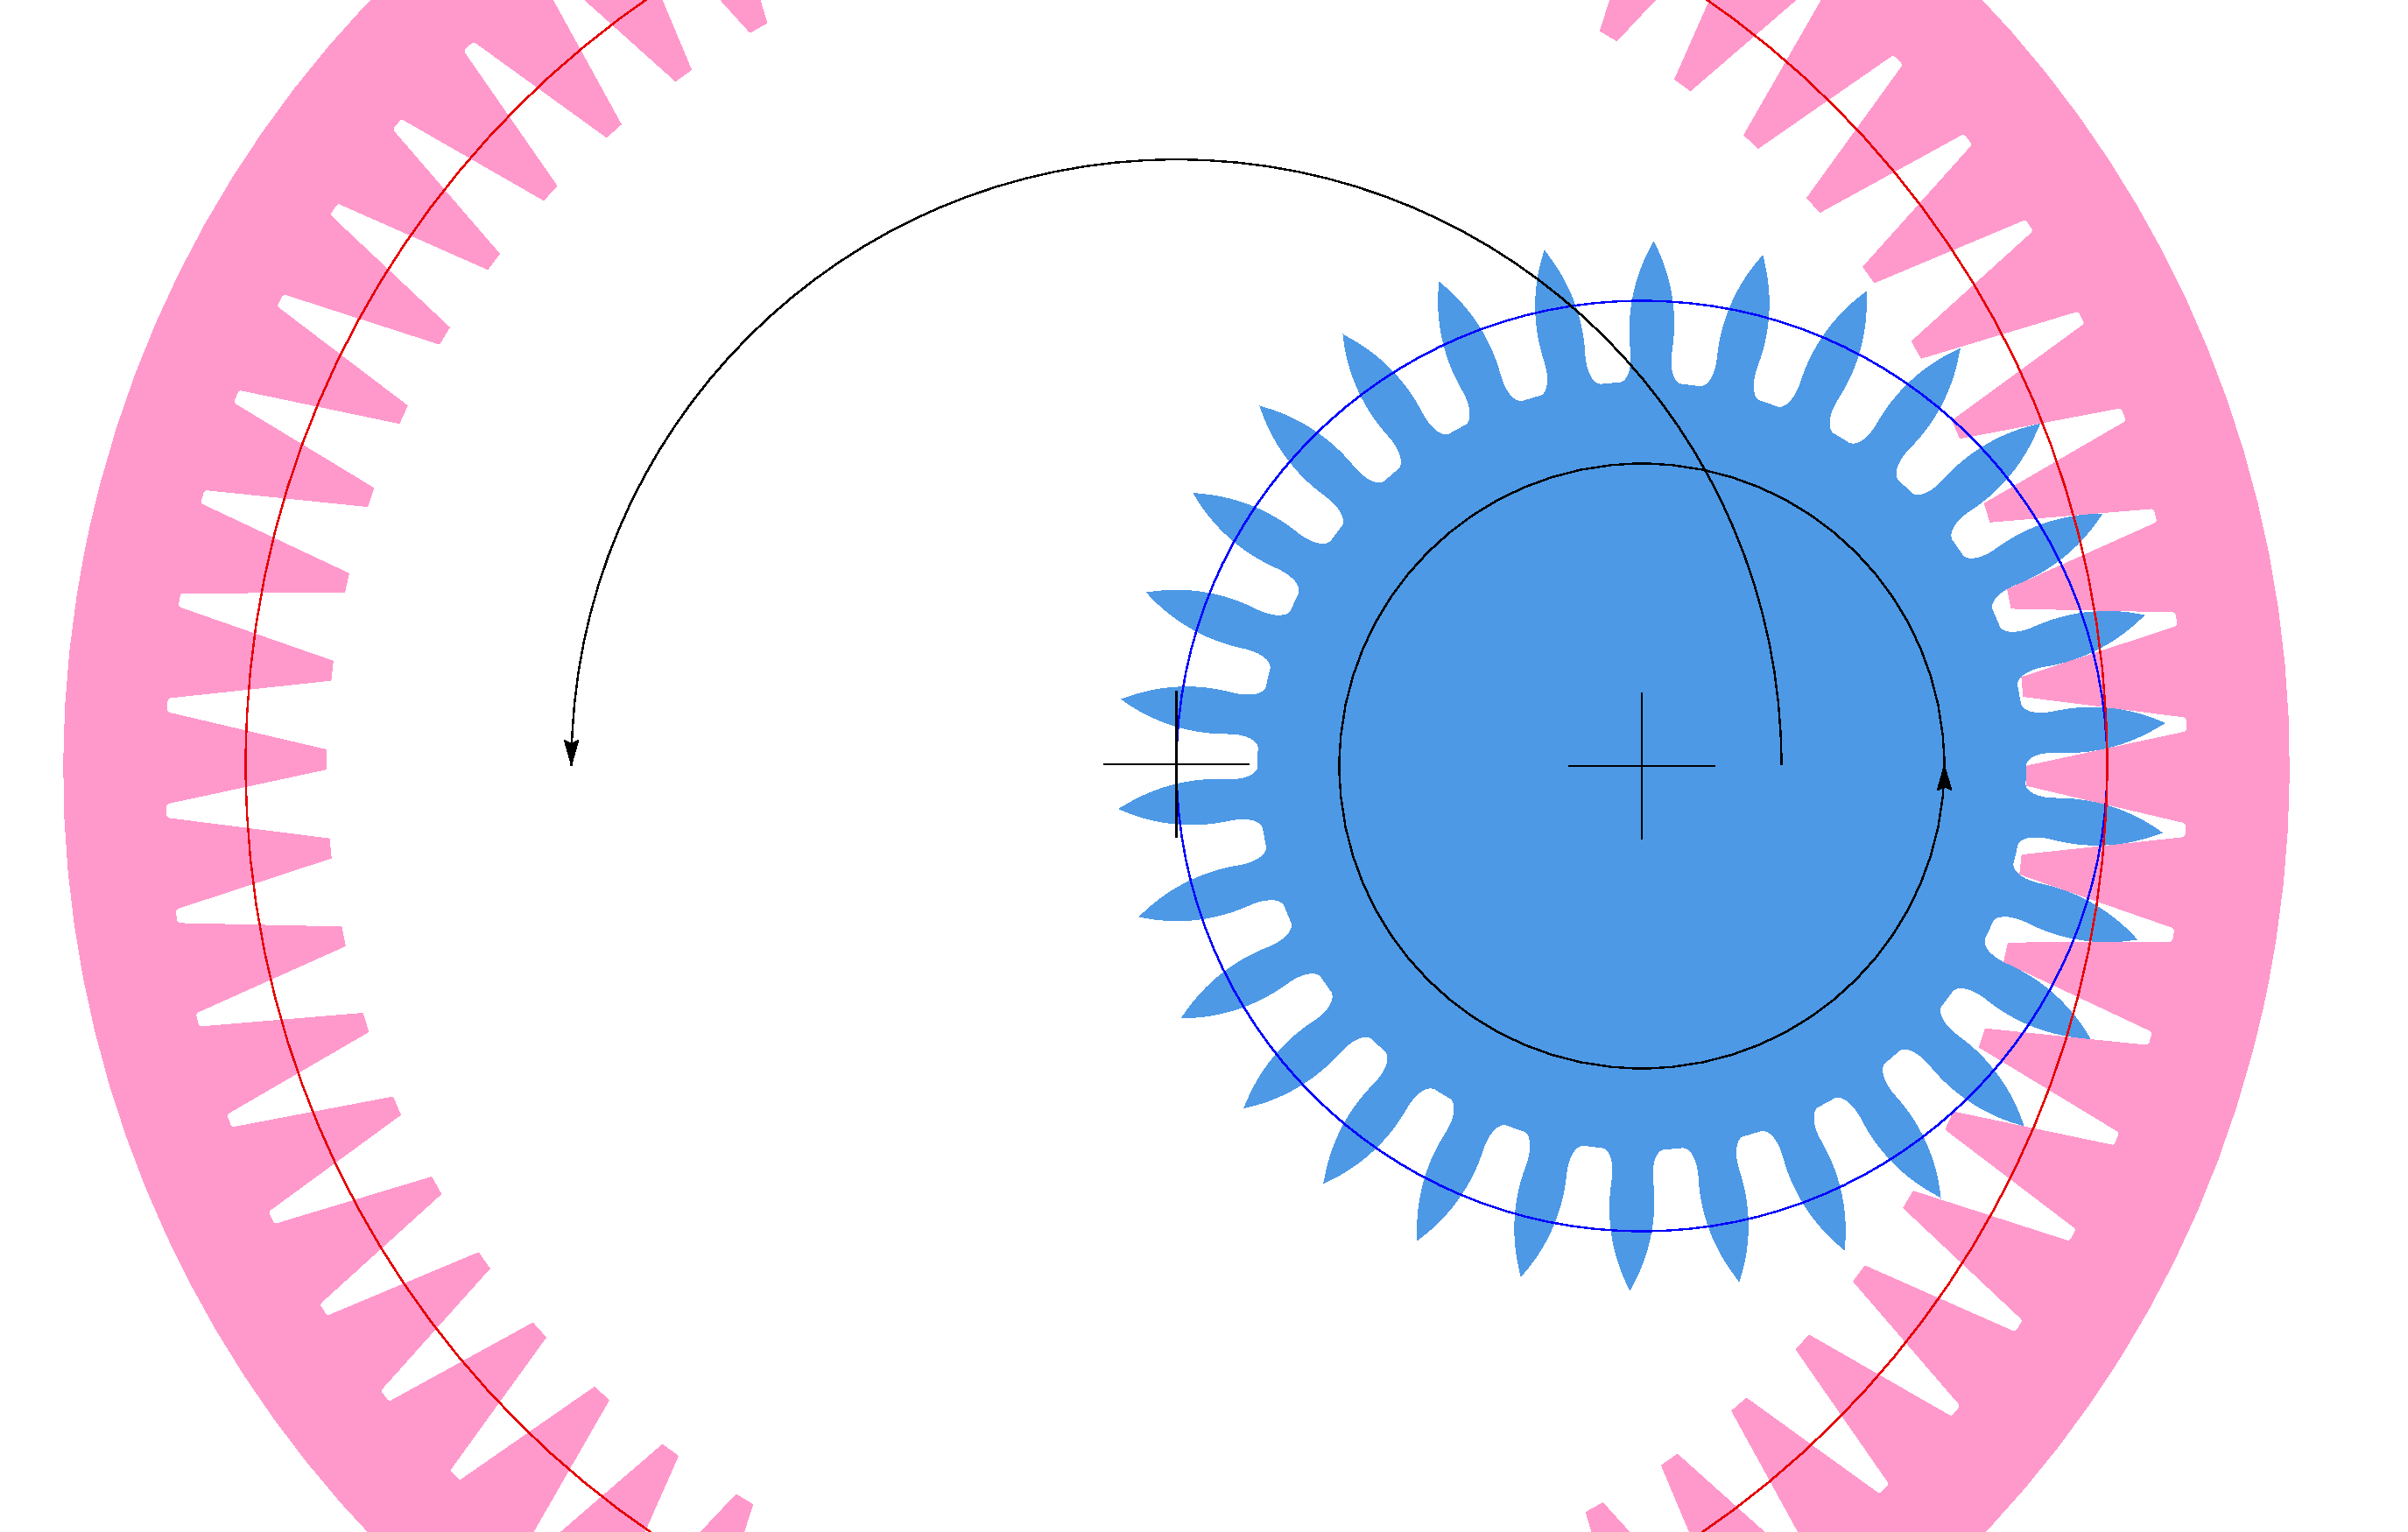
\includegraphics[width=\textwidth]{part2/ruote/FIG/ruote/squalo_interno.pdf}
\end{center}
\begin{picture}(0,0)(130,0)
\scriptsize{
\put(385,128){$\alpha=360^{\circ}$}
\put(200,130){$\beta=180^{\circ}$}
\put(346,155){famiglia b)}
\put(346,110){ruota 1 tagliata}
\put(230,47){ruota 2 creatrice}
}
\end{picture}
\vskip -7mm
      \caption{\em Dentatura ottenuta dall'utensile della figura \ref{fig:squalo}
con curvatura opposta.
I numeri di denti valgono $z_1=30$ e $z_2=60$.
}
 \label{fig:squalo_interno}
\end{figure}
In figura \ref{fig:squalo_interno} si accenna alla dentatura che
si otterrebbe per la famiglia b) di ruote complementari alla ruota 
azzurra della famiglia a) di figura \ref{fig:squalo}. Ovviamente, la ruota
appartenente a questa seconda famiglia b),
recante numero di denti pari alla ruota
 dentatrice (rosa)
di figura \ref{fig:squalo}, coinciderebbe con la dentatrice stessa e di
questa famiglia risulterebbe la maggiore\footnote{
Naturalmente, per la famiglia di ruote b) si potrebbero ottenere
ruote pi\`u grandi
della dentatrice di figura \ref{fig:squalo_interno} utilizzando come
utensile una qualsiasi ruota
appartenente alla famiglia a). Non presentiamo in queste note le dentature
interne, ma quello ora esposto rappresenta l'{\em escamotage} che consente
di eseguire dentature interne derivanti dalla dentiera creatrice {\em standard},
che \`e una cremagliera, quindi sicuramente di diametro maggiore rispetto
alla dentatura interna da eseguire.
}.
Ripetiamo che non siamo ancora in grado di valutare  se tutte le ruote della
famiglia a) siano o meno le {\em partner} cinematiche ideali delle ruote b),
ma il nostro fiuto ci convince che  siamo sulla buona strada.
Aggiungiamo, a questi procedimenti ingenui di taglio delle ruote dentate, due
precisazioni.
La prima: il taglio
della maggior parte delle ruote dentate avviene, da un punto di vista
concettuale, proprio nel modo in cui noi le abbiamo tagliate
nell'esperimento mentale, con qualche opportuno accorgimento pratico.
Siccome il materiale da tagliare, che \`e nella gran parte dei casi
acciaio al carbonio, non \`e ``morbido'', il processo di taglio deve avvenire
per asportazione di truciolo. Nei nostri due casi si dovrebbe operare
spostando la ruota creatrice, rosa, fuori dal piano,
per poi accostarla a quella da tagliare; a questo punto
riportarla nel piano, asportando in tal modo il materiale in eccesso
sulla ruota azzurra. Questo procedimento va ripetuto molte volte e a 
piccoli passi, cos\`i da simulare, durante il taglio, l'effettivo
processo di inviluppo continuo che avremmo col rotolamento, l'una
sull'altra, delle due primitive (le circonferenze delle ruote di frizione
riportate in colore rosso e blu). Da qui deriva la seconda precisazione.
Il movimento alternato dell'utensile, che \`e costretto,
uscendo dal piano, ad uscire di scena,
ci consente di avere delle fasi oziose dove siamo
liberi di imporre, alla ruota creatrice, spostamenti non basati sul
rotolamento delle primitive, ma che risultano utili per i nostri fini di taglio.
Infatti, normalmente, una volta guadagnato sulla
ruota creatrice un angolo $\Delta \beta$
corrispondente a $360 /z_2$, si torna indietro con questa 
ruota di tale quantit\`a. Operando in tale maniera, non siamo
costretti ad avere un utensile creatore con un numero di denti elevato,
anzi in genere basta un numero di denti modesto per creare ruote in
un vasto intervallo di numeri di denti. Anche noi ci siamo comportati
in questo modo per disegnare numericamente le nostre figure,
assicurandoci cos\`i di non rendere il codice
che le genera troppo pesante. Inoltre, il semplice movimento di creazione
per inviluppo, che consiste nel rotolamento delle due primitive, pu\`o
essere sostituito da qualsiasi movimento che rispetti tale moto relativo:
nelle nostre figure si \`e scelto di tenere ferma la ruota azzurra e di
movimentare la ruota creatrice di conseguenza. Gli angoli rappresentati
nelle figure \ref{fig:belbon}, \ref{fig:belbon_interno}, \ref{fig:squalo} e
\ref{fig:squalo_interno} si riferiscono esclusivamente al movimento
del creatore, in particolare alla sua rotazione $\beta$ e all'angolo
della porzione di ruota tagliata $\alpha$.
 
\noindent  Non \`e necessaria un'esperienza da meccanico consumato
per constatare  che i denti tagliati sulla ruota 1) di figura \ref{fig:squalo}
sono estremamente scavati alla base.
Notiamo anche che i contatti tra ruota tagliata e creatore e presumibilmente 
tra ruote a) e ruote b) si manifestano sia su superfici (le ruote
dentate possiedono uno spessore) sia su segmenti singolari, come mostrato
in figura \ref{fig:squalo}.
Tali contatti singolari sono in grado, da un punto di vista teorico,
di garantire il corretto e costante rapporto di trasmissione, \index{trasmissione!omocinetica}
che \`e un altro precetto (forte), il quarto.
Detti contatti non sono per\`o idonei a trasferire forze da un elemento
all'altro;
veniamo dunque al quinto precetto (forte):
nella trasmissione del movimento devono necessariamente
essere implicati contatti di strisciamento tra superfici
aventi raggio di curvatura del loro profilo, nel punto di contatto,
 ben diverso da zero. Vedremo
a breve che questo precetto ci porter\`a a considerare utili,
al fine della costruzione delle ruote dentate, esclusivamente opportune
coppie di profili
coniugati, la cui definizione viene rimandata al prossimo paragrafo.

\noindent Altre due intuizioni potrebbero balenarci in mente:
per prima cosa, ci sembra probabile che una riduzione
dell'altezza dei ``denti di squalo'' nella dentatrice possa essere un rimedio
per la forma dei denti
troppo sotto-tagliata alla base della ruota 1); la seconda osservazione
riguarda il raggio della ruota creatrice.
Infatti, qualora utilizzassimo una dentatrice
che rimanesse inalterata
una volta cambiata di segno la
sua curvatura, non avremmo pi\`u due famiglie di
ruote, ma una soltanto, le quali potrebbero (forse) ingranare tutte
quante tra loro e questo, quello cio\`e di ridurre le famiglie di ruote da due
a una, lo diamo come sesto precetto (debole)\footnote{Chi vuole
pu\`o trovare nel capitolo \ref{ruotecy} 
la descrizione di particolari ruote a profilo
cicloidale per le quali si tollera (o si richiede)
la presenza di due famiglie di ruote.}.
Tale simmetria  dell'utensile creatore si chiama
{\em auto-complementarit\`a}\index{auto-complementarit\`a} e
ci conduce  a un creatore a
dentiera rettilinea coi fianchi dei denti pure costituiti da segmenti di retta.
Ma tutte queste intuizioni, che vengono in mente per lo pi\`u a chi le ruote
dentate gi\`a le conosce, 
andrebbero poste in ordine. Per questo siamo costretti
 a toglierci dal nostro comodo sentiero intuitivo
e addentrarci, per poi uscirne il prima possibile, nel pi\`u impervio cammino
che porta alla costruzione dei cosiddetti {\em profili coniugati di
assortimento}\index{profili!di assortimento}.

\section{Costruzione di Profili Coniugati di Assortimento} \label{prof_con}

\noindent Questo paragrafo tratta un problema di cinematica riportato
sulla maggior parte dei
 libri di Meccanica Applicata alle Macchine, ma anche su
alcuni testi di Meccanica Razionale. Prima di 
impostare la definizione dei profili coniugati e di presentare una soluzione
per il loro ottenimento, una volta date le primitive del moto, avvertiamo
il lettore che di tutto questo studio si utilizzeranno soltanto un paio di
conclusioni, legate a due casi molto particolari,
e che tali risultati saranno 
esposti, in riassunto, all'inizio del prossimo paragrafo, al quale rimandiamo
i lettori che non sentono particolare inclinazione per questo argomento.

\noindent Ma cosa sono due {\em profili coniugati}\index{profili!coniugati}?
Due curve regolari qualsiasi possono essere messe tra loro in una
infinit\`a di relazioni reciproche le quali, determinando il loro
posizionamento e il loro movimento relativo,
le rendono tra loro coniugate. 
Come vedremo a breve, ciascuna di queste infinite possibili relazioni, di
natura matematica, che determina il movimento di una curva rispetto all'altra,
deve per\`o possedere alcune caratteristiche (poche) particolari.
Siano $\sigma_1(t)\equiv [\sigma_1(t)_x,\sigma_1(t)_y]^T$ e
$\sigma_2(\tau)\equiv [\sigma_2(\tau)_x,\sigma_2(\tau)_y]^T$,
nel piano cartesiano $(x,y)$, due curve continue e prive di singolarit\`a
in due dati intervalli dei loro parametri, $t$ e $\tau$.
Si scelga ora una funzione, $\tau=f(t)$ definita negli intervalli di interesse,
che mette in corrispondenza biunivoca due intervalli finiti
di coppie di punti appartenenti alle due curve. La relazione tra i due
parametri, $f()$, lega pertanto tra loro i punti
$\sigma_1(t)$ e $\sigma_2(f(t))$ che saranno i candidati
alla coniugazione andando, dopo opportune trasformazioni, a coincidere.
Inoltre, la stessa funzione $f()$ metter\`a naturalmente in relazione anche
le inclinazioni delle tangenti alle curve stesse, che
indicheremo con $\alpha_1(t)$ e $\alpha_2(f(t))$:
anche questi due valori dovranno coincidere nel punto
di coniugazione tra i profili.
Per ora, richiediamo soltanto che $f()$ sia continua e vedremo in seguito
se a tale funzione siano da richiedere o meno altre restrizioni.
Utilizziamo la relazione tra i due parametri per eseguire
alcune {\em trasformazioni piane}\index{trasformazioni piane} di una delle due
curve. In questa sede si \`e deciso ad arbitrio di operare su $\sigma_2$, per
ottenere da tali trasformazioni (continue) la sua coniugata $\sigma_1$.
Procediamo nel modo
seguente; disegnata $\sigma_1(t)$, proponiamo la famiglia di curve
${\sigma_2(\tau)}_t$, che invilupper\`a $\sigma_1$,
mediante la seguente relazione che consta di quattro trasformazioni piane,
le quali legano tra loro le due curve
\begin{equation}
{\sigma_2(\tau)}_t = 
 {\bm T}[\sigma_1(t)]\cdot {\bm R}[\alpha_1(t)]
\cdot{\bm R}[-\alpha_2(f(t))]\cdot
 {\bm T} [-\sigma_2(f(t))]\cdot \sigma_2(\tau)\,.
\label{eq:inviluppo}
\end{equation}

\begin{figure}[hbt]
\begin{center}
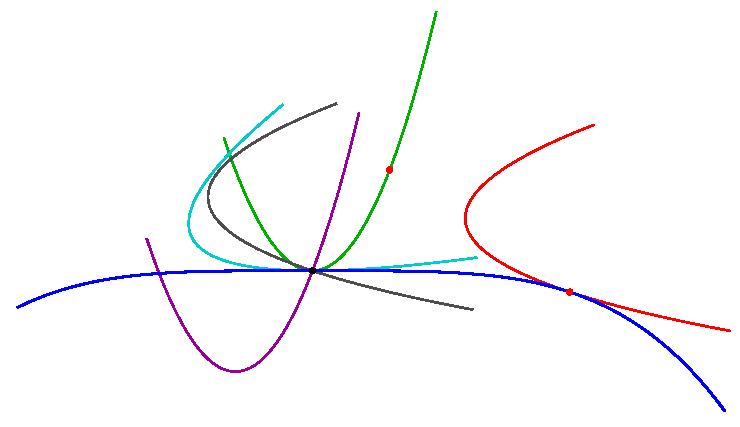
\includegraphics[width=0.8\textwidth]{part2/ruote/FIG/ruote/profili_coniugati_definizione_steps.pdf}
\end{center}
\begin{picture}(0,0)(0,0)
\scriptsize{
\put(318,27){$\sigma_1(t)$}
\put(259,84){$\sigma_1(c)$}
\put(209,186){$\sigma_2(\tau)$}
\put(197,182){$a)$}
\put(176,152){$b)$}
\put(215,75){$d)$}
\put(210,95){$c)$}
\put(315,68){$e)$}
\put(192,125){$\sigma_2(f(c))$}
\put(161,68){$0,0$}
\put(159,74){\rotatebox{120}{$\longrightarrow$}}
\put(75,40){$\sigma_2'(\tau)= {\bm T} [-\sigma_2(f(c))]\cdot \sigma_2(\tau)$}
\put(20,156){$\sigma_2''(\tau)={\bm R}[-\alpha_2(f(c))]\cdot \sigma_2'(\tau)$}
\put(132,150){{$\longrightarrow$}}
\put(180,53){$\sigma_2'''(\tau)={\bm R}[\alpha_1(c)]]\cdot \sigma_2''(\tau)$}
\put(215,62){\rotatebox{130}{$\longrightarrow$}}
\put(236,147){$ \sigma_2(\tau)_c={\bm T}[\sigma_1(t)]\cdot \sigma_2'''(\tau)$}
}
\end{picture}
\vskip -7mm
      \caption{\em
Le quattro trasformazioni della formula \ref{eq:inviluppo}.
}
 \label{fig:profili_coniugati_definizione_steps}
\end{figure}
\noindent Le trasformazioni ${\bm T}$ e ${\bm R}$ sono rispettivamente
le traslazioni e le rotazioni nel piano. Esse agiscono sui vettori colonna
dei punti di $\sigma_2$. In particolare, le traslazioni ${\bm T}$ accetteranno
due parametri, dati dai punti $[x,y]^T$ della
curva che contengono come argomento, mentre le rotazioni ${\bm R}$ ne
accetteranno uno solo: tale parametro
\`e l'angolo compreso tra la tangente alla curva, cui l'argomento della
rotazione si riferisce, e una direzione arbitraria e fissa (nelle
nostre figure, quella verticale).
Allo scopo di chiarire la trasformazione operata in \ref{eq:inviluppo}
illustriamo in figura 
\ref{fig:profili_coniugati_definizione_steps} un esempio dove 
la curva $\sigma_1$, riportata in blu, \`e, nella fattispecie, una parabola di
quarto grado rovesciata con vertice nell'origine, mentre la $\sigma_2$, verde,
consiste in una parabola di secondo grado, sempre col vertice nell'origine
e asse verticale.
Infine, la funzione che lega i due parametri \`e semplicemente data
da $\tau=0.3t$. Rimarchiamo che, nonostante tutte le scelte arbitrarie
operate al fine di ottenere la figura
\ref{fig:profili_coniugati_definizione_steps} riflettano una decisa semplicit\`a
(parabole centrate, funzione lineare che lega i due parametri), ci\`o non
inficia la generalit\`a dell'esempio, come vedremo pi\`u avanti, dove lo stesso
codice che genera la figura appena citata viene impiegato per
la generazione di profili coniugati pi\`u complessi. 
Consideriamo la trasformazione \ref{eq:inviluppo} per un valore del parametro
$t=c$.  Tale parametro individua i punti $\sigma_1(c)$ e $\sigma_2(f(c))$,
in rosso nella figura \ref{fig:profili_coniugati_definizione_steps}.
Analizziamo la \ref{eq:inviluppo} partendo da
destra e mettendo in fila le operazioni necessarie per avere le due
curve coniugate nel punto di $\sigma_1(c)\equiv\sigma_2(f(c))$.
Il termine pi\`u a destra, $\sigma_2(\tau)$,
sar\`a semplicemente la curva mobile a), di colore verde, gi\`a citata poc'anzi.
La trasformazione $ {\bm T} [-\sigma_2(f(c))] $ \`e una traslazione che porta il 
punto di $\sigma_2$ destinato ad essere coniugato (col punto ``c-esimo'' di
$\sigma_1$) nell'origine degli assi. Il risultato \`e rappresentato dalla 
curva di colore violetto b) e nome $\sigma_2'(\tau)$.
L'allineamento degli spazi tangenti alle due curve, nei
punti di coniugazione (di parametri $c$ e $f(c)$), avviene in due fasi.
Applichiamo alla $\sigma_2'(\tau)$ una prima rotazione 
di segno contrario alla tangente a $\sigma_2'$ in $\tau=f(c)$, ottenendo in tal
modo $\sigma_2''(\tau)={\bm R}[-\alpha_2(f(c))]\sigma_2'(\tau)$,
parabola c), riportata in colore azzurro chiaro. Applichiamo quindi una seconda
rotazione, pari all'inclinazione della tangente a $\sigma_1$ in $c$, ottenendo
cos\`i $\sigma_2'''(\tau)={\bm R}[\alpha_1(c)]\cdot\sigma_2''(\tau)$,
che \`e la parabola in colore grigio d).
\begin{figure}[hbt]
\begin{center}
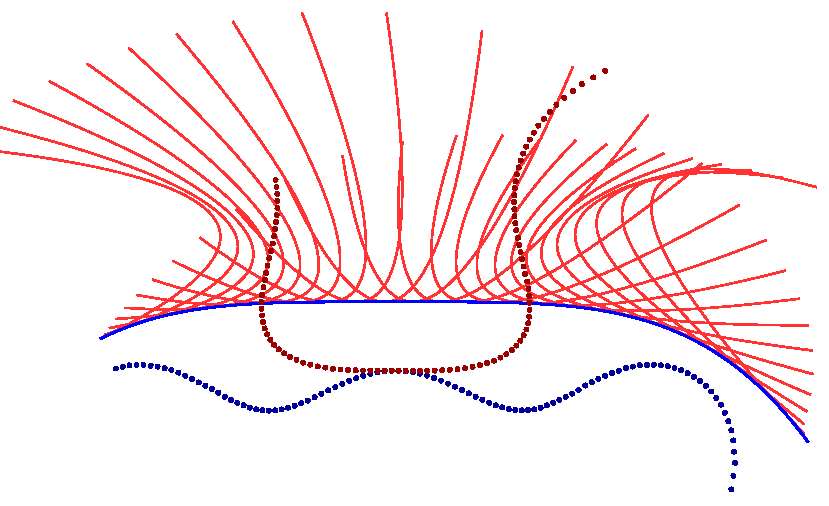
\includegraphics[width=0.8\textwidth]{part2/ruote/FIG/ruote/profili_coniugati_definizione_a.pdf}
\end{center}
\begin{picture}(0,0)(0,0)
\scriptsize{
\put(315,42){$\sigma_1$}
\put(206,189){$\sigma_2$}
\put(67,66){$\lambda_1$}
\put(251,176){$\lambda_2$}
}
\end{picture}
\vskip -7mm
      \caption{\em
Profili coniugati: inviluppo e relative polari.
}
 \label{fig:profili_coniugati_definizione_a}
\end{figure}
Finalmente, non rimane
che traslare la curva $\sigma_2'''(\tau)$, 
la quale si trova ora col suo ``c-esimo'' punto in (0,0) e con la tangente in
quel punto inclinata come la tangente a $\sigma_1(c)$,
sul punto di coniugazione con $\sigma_1$, e questo si esegue
mediante la traslazione $\sigma_2(\tau)_c={\bm T}[\sigma_1(c)]\sigma_2'''(\tau)$,
ottenendo in tal modo la parabola e).
Il risultato di queste operazioni, al variare del punto
di coniugazione, cio\`e al variare di $c$,  \`e quello mostrato in figura
\ref{fig:profili_coniugati_definizione_a}. La parabola di colore
rosso, che crea l'inviluppo di $\sigma_1$, viene rappresentata,
onde evitare un eccessivo
appesantimento dell'immagine, soltanto in una ventina di posizioni,
rendendo comunque perfettamente l'idea del processo di inviluppo.
Da un punto di vista matematico, le condizioni necessarie e sufficienti
affinch\'e la $\sigma_2$, durante il suo movimento, inviluppi la curva
$\sigma_1$ sono due, e precisamente \`e richiesto che i punti omologhi
delle due curve coincidano per tutti i valori omologhi dei due parametri (nei
due intervalli di interesse) e che, in tali punti, anche le tangenti
alle due curve siano la stessa retta\footnote
{
L'inviluppo di una curva, espressa
come $\phi(x,y,\lambda)=0$ dove $\lambda$ \`e il parametro che la muove nel
piano, si ottiene eliminando il parametro stesso
dal sistema
\begin{equation}
\begin{cases}
\phi(x,y,\lambda)=0 \\
\displaystyle \frac{\partial \phi(x,y,\lambda)} {\partial\lambda}=0\,,
\end{cases}
\nonumber
\end{equation}

\noindent il che \`e del tutto equivalente a quanto da noi richiesto.
}.

\vskip .2cm
\footnotesize
\noindent Si intuisce facilmente che entrambe queste condizioni sono assicurate
dal procedimento descritto dalla \ref{eq:inviluppo} e illustrato in figura
\ref{fig:profili_coniugati_definizione_a} ma, rischiando di passare per
pedanti, ne riportiamo comunque la dimostrazione.
Quanto alla prima condizione, cio\`e la prescrizione che le due curve
$\sigma_2$ e l'inviluppo creato dalla \ref{eq:inviluppo}, coincidano,
essa deriva con semplicit\`a da ci\`o che
abbiamo discusso circa la  struttura della \ref{eq:inviluppo} stessa.
Considerando infatti un valore del
parametro $t=c$ \hspace{.1 cm} e, di conseguenza, $\tau=f(c)$, avremo
\begin{equation}
{\sigma_2(f(c))}_c = 
 {\bm T}[\sigma_1(c)]\cdot {\bm R}[\alpha_1(c)]\cdot{\bm R}[-\alpha_2(f(c))]\cdot
 {\bm T} [-\sigma_2(f(c))]\cdot \sigma_2(f(c))\,.
\label{eq:dimost_x}
\end{equation}
\noindent Ma considerando la prima (si parte sempre da destra) delle
trasformazioni della \ref{eq:dimost_x} abbiamo
\begin{equation}
{\bm T} [-\sigma_2(f(c))]\cdot \sigma_2(f(c))=(0,0)^T.
\label{eq:dimost_x1}
\end{equation}
\noindent Pertanto, tenendo presente che le rotazioni non hanno effetto sul vettore
nullo, avremo
\begin{equation}
{\sigma_2(f(c))}_t = 
 {\bm T}[\sigma_1(c)]\cdot {\bm R}[\alpha_1(c)]\cdot{\bm R}[-\alpha_2(f(c))]\cdot
 \left(\begin{matrix} 0 \\ 0 \\ \end{matrix}\right)= 
 {\bm T}[\sigma_1(c)]\cdot 
 \left(\begin{matrix} 0 \\ 0 \\ \end{matrix}\right)= 
{\sigma_1(c)}\,. 
\label{eq:dimost_p}
\end{equation}
\noindent Poco pi\`u laboriosa \`e la dimostrazione
della coincidenza delle tangenti alle due curve nel punto di coniugazione.
Analizziamo, a tale proposito, in che modo la \ref{eq:dimost_x}
trasforma il punto infinitamente vicino a quello di parametro $c$
della curva $\sigma_2$. Tale punto risulta individuato dalla seguente espressione
differenziale
\begin{equation}
\sigma_2(f(c)+{\rm d}\tau))=\sigma_2(f(c))+
{{\rm d}{\sigma_2}\over{{\rm d}\tau}}\bigr|_{(f(c))} 
{\rm d} \tau \,, 
\label{eq:dimost_t1}
\end{equation}
\noindent dove il termine ${{\rm d}{\sigma_2}\over{{\rm d}\tau}}\bigr|_{(f(c))}
{\rm d} \tau$ rappresenta un vettore infinitesimo
diretto come la tangente alla $\sigma_2$ nel punto $\sigma_2(f(c))$.
Chiamiamo con $\bm \delta_c$ il vettore infinitesimo 
\begin{equation}
{\bm \delta_c}= \sigma_2(f(c)+{\rm d}\tau)_c- \sigma_2(f(c))_c\,,
\label{eq:vett_inf}
\end{equation}
\noindent intendendo
con i due addendi a destra del segno di uguaglianza l'applicazione della
\ref{eq:dimost_x} sia al punto $\sigma_2(f(c)+{\rm d}\tau))$, sia
al punto $\sigma_2(f(c))$. Data la linearit\`a degli operatori
presenti nella
\ref{eq:dimost_x} vale, per gli operandi, la propriet\`a distributiva
\begin{equation}
{\bm T}()\cdot{\bm R}()\cdot {\bm R}()\cdot{\bm T}()\cdot({\bm a}+{\bm b})=
{\bm T}()\cdot{\bm R}()\cdot {\bm R}()\cdot{\bm T}()\cdot{\bm a}+
{\bm T}()\cdot{\bm R}()\cdot {\bm R}()\cdot{\bm T}()\cdot{\bm b}\,.
\end{equation}

\noindent Ci\`o che rimane dall'applicazione della \ref{eq:dimost_x}
risulta quindi essere
\begin{equation}
{\bm \delta_c} =
 {\bm T}[\sigma_1(c)]\cdot {\bm R}[\alpha_1(c)]\cdot{\bm R}[-\alpha_2(f(c))]
\cdot 
 {\bm T} [-\sigma_2(f(c))]
	\cdot (
{{\rm d}{\sigma_2}\over{{\rm d}\tau}}\bigr|_{(f(c))} 
{\rm d} \tau )\,.
\label{eq:dimost_x3}
\end{equation}
\noindent Sarebbe tedioso ripercorrere per gradi le operazioni
illustrate in figura \ref{fig:profili_coniugati_definizione_steps}, pertanto ci
limitiamo qui a seguire velocemente le trasformazioni del vettore tangente infinitesimo
${{\rm d}{\sigma_2}\over{{\rm d}\tau}}\bigr|_{(f(c))}
{\rm d} \tau$. Ricordando che si parte sempre da destra, esso si muove, mediante
il primo operatore di traslazione,
nell'origine degli assi. Quindi, tramite le due rotazioni, tale vettore
si dispone come la
tangente alla curva $\sigma_1$ nel punto $t=c$. Infine,
mediante l'ultima traslazione $\bm \delta_c$, esso si ritrover\`a
proprio in tale punto
di $\sigma_1$. Risulta cos\`i provato che anche i vettori tangenti alla
$\sigma_2$ diventano, dopo il procedimento di coniugazione, altrettanti
vettori tangenti alla curva $\sigma_1$.



\vskip .2cm
\normalsize
\noindent Abbiamo gi\`a ammesso che le due dimostrazioni, test\'e sviluppate e
stampate con tipi minori, si
presentano come leggermente superflue, essendo il procedimento contenuto
nella \ref{eq:inviluppo}, ed esposto graficamente in
figura \ref{fig:profili_coniugati_definizione_steps}, intrinsecamente volto
ad ottenere la coniugazione dei profili. Tali dimostrazioni ci sono per\`o
utili per meglio circoscrivere i vincoli matematici ai quali $\sigma_1$,
$\sigma_2$ e $f()$ devono sottostare. Affinch\'e si possa manifestare
la coincidenza nei punti di coniugazione, il che equivale alla possibilit\`a
di scrivere la \ref{eq:dimost_x}, la funzione $\tau=f(t)$, che lega i
parametri delle due curve, deve essere definita per tutti i valori di $t$
nell'intervallo di
interesse. Solo questo? S\`i, soltanto questo. Ad essa non \`e chiesto n\'e
di essere monotona n\'e di sottostare
a restrizioni sulle sue derivate, anzi non \`e richiesta neppure
la sua derivabilit\`a. Deve essere chiaro per\`o che ragionando
in questo modo, cio\`e ammettendo che $f()$ possa manifestare qualsiasi
bizzarria, \`e probabile che non si otterranno profili coniugati con
caratteristiche adatte all'impiego nella
meccanica delle macchine. Per quanto riguarda la possibilit\`a
di scrivere la \ref{eq:dimost_t1}, che costituisce la base della seconda 
dimostrazione, circa la coincidenza delle tangenti ai profili, \`e richiesto
che $\sigma_2$, e di conseguenza $\sigma_1$, siano differenziabili, e nulla pi\`u.
Certo, si intuisce con facilit\`a
che aggiungendo altre restrizioni sia ai profili (immaginandoli
ad esempio curve regolari e lisce), sia
alla funzione che lega tra loro i due parametri (che si potrebbe ipotizzare
continua e monotona), si intuisce, dicevamo, che le speranze di ottenere
profili coniugati lisci, privi di singolari\`a e interferenze 
sarebbe superiore.
Ma, come vedremo, tutte queste apprensioni circa la bont\`a dei profili e della
relazione cinematica che li fa scorrere l'uno sull'altro sono fuori luogo nella
meccanica applicata, dove saremo costretti ad ammettere
che i (il?) soli profili interessanti sono anche estremamente semplici.  
Una volta nota, tramite la \ref{eq:inviluppo}, la traiettoria
di due punti qualsiasi appartenenti alla curva $\sigma_2$, chiamiamoli
$\sigma_2(\tau_1)$ e $\sigma_2(\tau_2)$, mentre essa inviluppa $\sigma_1$,
possiamo individuare, al variare del parametro $t$,
le normali a tali traiettorie. Per ciascun valore di $t$,
dall'intersezione di dette normali, otterremo
il centro istantaneo di rotazione di $\sigma_2$. Il luogo geometrico
delle tracce dei centri istantanei di rotazione di $\sigma_2$
si chiama {\em polare fissa}\index{polare!fissa} e verr\`a indicata con $\lambda_1$.
La {\em polare mobile}\index{polare!mobile}, $\lambda_2$,
si ottiene invece lasciando che, una volta individuato il
centro istantaneo di rotazione per un dato valore di
$t$, tale punto venga trascinato
dal piano mobile. \`E sottinteso che, come sempre accade coi moti relativi,
le parti possono essere 
invertite tenendo ferma $\sigma_2$ e facendo muovere $\sigma_1$. Durante tale moto
le polari verranno a scambiarsi tra loro ottenendo, in questo caso, la 
precedente polare mobile come attuale polare fissa.
Polare fissa e polare mobile sono a contatto
tra loro nel centro istantaneo di rotazione corrispondente ad un 
dato valore del parametro $t$ e il loro movimento relativo \`e di puro rotolamento.
In figura \ref{fig:profili_coniugati_definizione_a} sono rappresentate
le polari del moto di $\sigma_2$, fissa e mobile, mediante un centinaio
di punti scelti dal migliaio a nostra disposizione tramite
il codice che genera la stessa figura
\ref{fig:profili_coniugati_definizione_a} e le altre
\ref{fig:profili_coniugati_definizione_b} e
\ref{fig:profili_coniugati_definizione_b1} e che,
qualora fossero tutti disegnati, avrebbero reso continue tali curve.
La rappresentazione
di un minor numero di punti consente di rendere l'idea,
tramite le distanze reciproche tra i punti stessi,
della equivalenza delle lunghezze di tratti
omologhi delle due polari, equivalenza implicata dal rotolamento.
In generale le polari sono curve poco intuitive e possono presentare
discontinuit\`a e contenere punti impropri.

\begin{figure}[hbt]
\centering
\begin{minipage}[b]{0.45\textwidth}
\centering
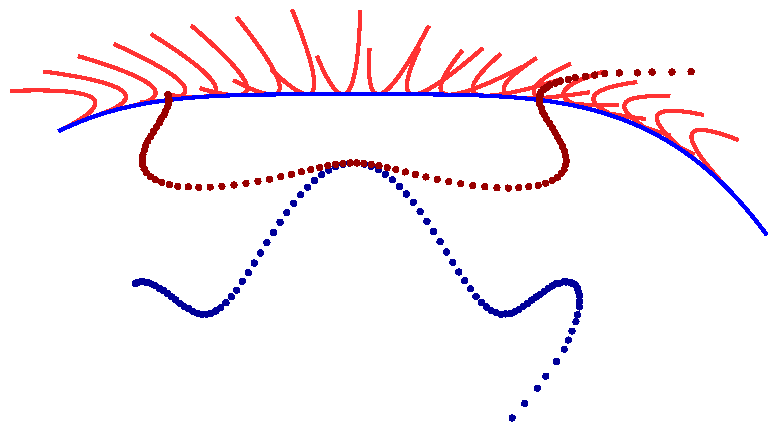
\includegraphics[width=0.9\textwidth]{part2/ruote/FIG/ruote/profili_coniugati_definizione_b.pdf}
\begin{picture}(0,0)(130,0)
\scriptsize{
\put(123,33){$\sigma_1$}
\put(46,83){$\sigma_2$}
\put(-3,26){$\lambda_1$}
\put(114,68){$\lambda_2$}
}
\end{picture}
      \caption{\em
Curva $\sigma_2$ in scala ridotta e nuove polari.
}
 \label{fig:profili_coniugati_definizione_b}
\end{minipage}\hfill
\begin{minipage}[b]{0.45\textwidth}
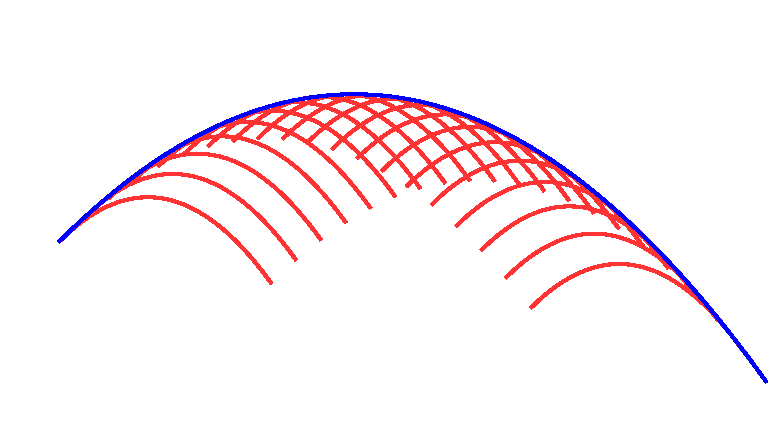
\includegraphics[width=0.9\textwidth]{part2/ruote/FIG/ruote/profili_coniugati_definizione_b1.pdf}
\begin{picture}(0,0)(130,0)
\scriptsize{
\put(124,5){$\sigma_1$}
\put(30,23){$\sigma_2$}
\put(-19,8){\rotatebox{-90}{$\longrightarrow$}}
\put(-13,-3){polare fissa e polare mobile all'infinito}
}
\end{picture}
      \caption{\em
Profili coniugati traslanti.
      }
 \label{fig:profili_coniugati_definizione_b1}
\end{minipage}
\end{figure}


\noindent Una situazione non molto dissimile da quella di figura 
\ref{fig:profili_coniugati_definizione_a} \`e quella rappresentata in
\ref{fig:profili_coniugati_definizione_b}, dove la curva $\sigma_2$ \`e
riportata in scala minore e $\tau=0.07t$, allo scopo di mostrare quale
cambiamento macroscopico subiscono le due polari del moto a fronte di un
cambiamento, apparentemente leggero, di uno dei due profili coniugati.
In figura \ref{fig:profili_coniugati_definizione_b1} viene
invece mostrata
una curva $\sigma_2$ che inviluppa, tramite un moto esclusivamente 
traslatorio, la curva $\sigma_1$, sua simile ma in scala maggiore. Per questo
esempio \`e stata infatti scelta una funzione $f()$, che lega i due parametri,
tale da portare a coniugazione i punti delle due curve aventi, a priori,
 la stessa
tangente. \`E proprio questo il motivo che rende traslatorio il moto di
inviluppo e che manda le polari del moto all'infinito rendendole
due segmenti di rette improprie la cui direzione coincide con quella di
spostamento del profilo  $\sigma_2$. I profili coniugati che abbiamo finora analizzato sono
stati ottenuti tramite curve $\sigma_2(\tau)$ molto semplici,
in pratica delle parabole.  Altrettanto semplici sono
i legami $\tau=f(t)$ che definiscono, tramite la $\sigma_1(t)$,
le leggi degli spostamenti di $\sigma_2$.  In questo modo,
gli inviluppi ottenuti somigliano a oggetti effettivamente
utilizzabili nella meccanica delle macchine.
\begin{figure}[hbt]
\begin{center}
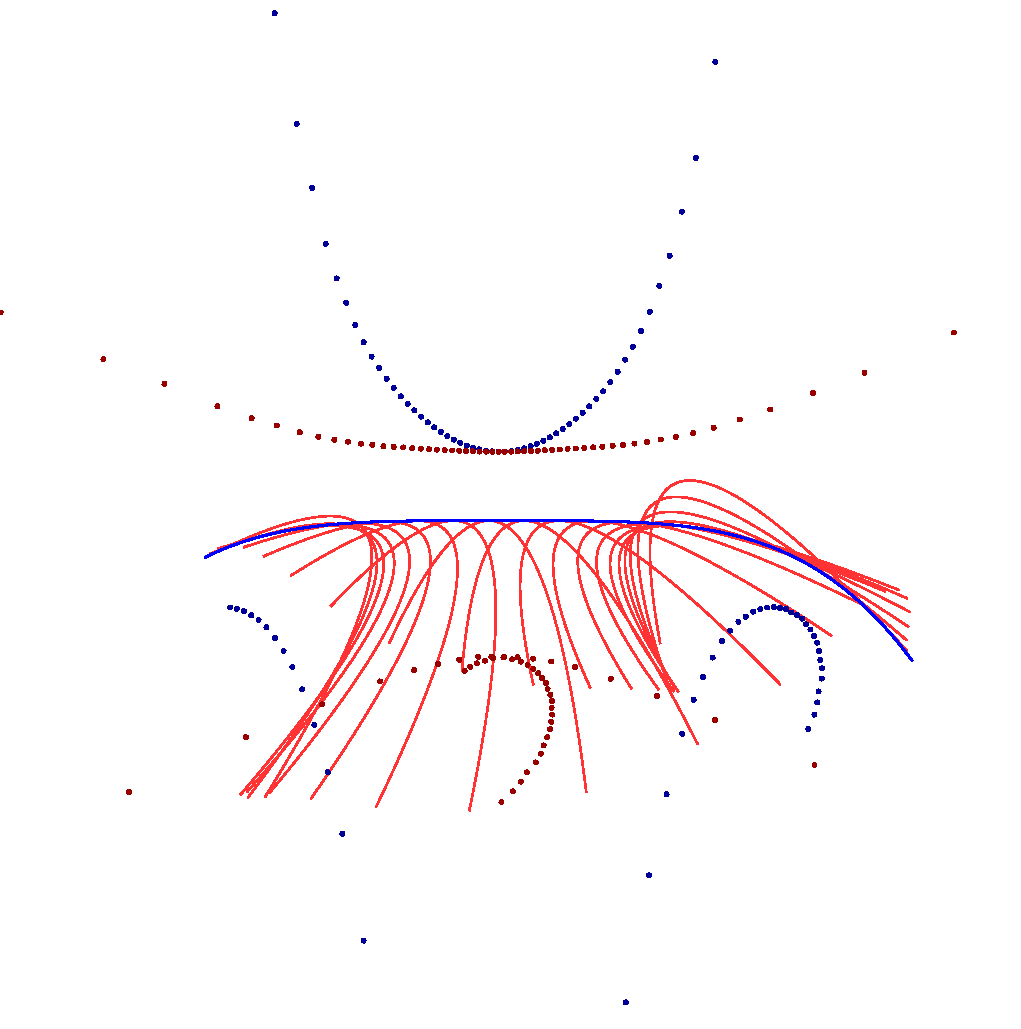
\includegraphics[width=0.8\textwidth]{part2/ruote/FIG/ruote/profili_coniugati_definizione_c.pdf}
\end{center}
\begin{picture}(0,0)(0,0)
\scriptsize{
\put(292,123){$\sigma_1$}
\put(198,87){$\sigma_2$}
\put(26,228){$\lambda_1$}
\put(62,92){$\lambda_1$}
\put(269,98){$\lambda_1$}
\put(103,313){$\lambda_2$}
\put(201,33){$\lambda_2$}
\put(129,50){$\lambda_2$}
}
\end{picture}
\vskip -5mm
      \caption{\em
Profili coniugati che si intersecano e polari discontinue.
}

 \label{fig:profili_coniugati_definizione_c}
\end{figure}
Come abbiamo per\`o ripetuto altre volte, la teoria dei profili coniugati
non mette restrizioni, se non
molto blande, alle tre entit\`a matematiche test\'e menzionate.
Per esempio, le curvature di $\sigma_1$ e  $\sigma_2$ possono essere
tali che, combinate alla funzione $f()$, producano inviluppi che 
si intersecano con le curve che li generano. In questi casi,
le polari del moto presentano spesso discontinuit\`a e punti
all'infinito,
come mostra la figura \ref{fig:profili_coniugati_definizione_c}.
Nel caso riportato in figura,
le curve $\sigma_1$ e $\sigma_2$ sono ancora parabole,
quindi curve semplici e regolari, e la funzione che lega i parametri delle due
curve \`e ancora $\tau=0.3t$. Ma le curvature dei due profili
risultano tra loro ``incompatibili''. Ben inteso, da un punto di
vista puramente matematico tutto fila liscio come sempre.
Nella tecnica, per\`o, tali profili non possono essere utilizzati
per trasmettere il  movimento o per altre funzioni concrete
quindi, per noi ingegneri,
rimangono curiosit\`a che appartengono alla teoria.
Nella figura
si possono anche vedere tutti gli spezzoni delle due polari per le quali
si intravedono gli asintoti che indicano le direzioni
dei loro punti impropri.
Capovolgiamo il problema. Supponiamo di conoscere le polari
del moto relativo, e investighiamo la possibilit\`a
di trovare due profili tra loro coniugati. Dettando le polari
la legge geometrica del moto relativo
del  piano mobile rispetto a quello fisso, ad ogni curva appartenente
al primo corrisponder\`a il relativo inviluppo sul secondo,
il quale, del profilo mobile, sar\`a anche il profilo coniugato.
\begin{wrapfigure}{r}{0.55\textwidth}
      \begin{center}
      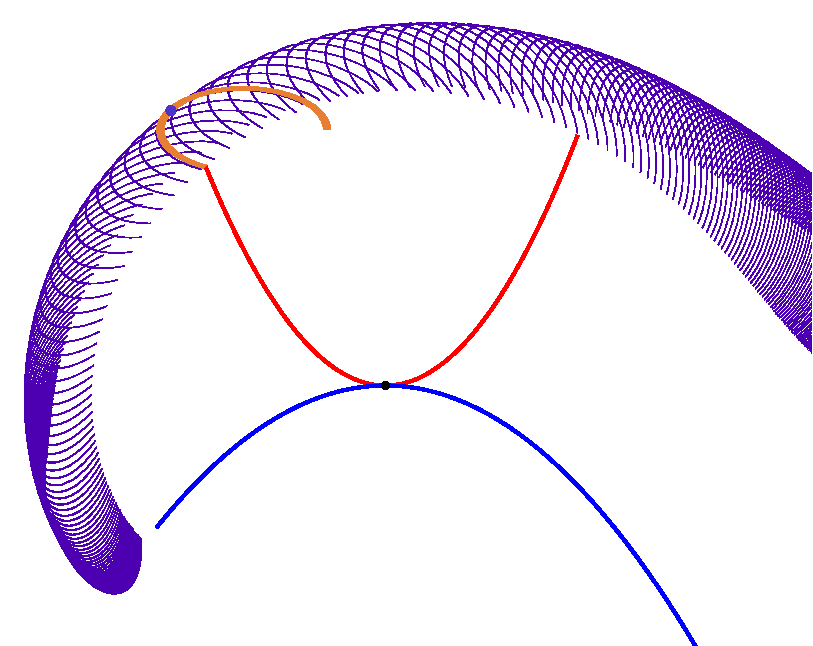
\includegraphics[width=0.50\textwidth]{part2/ruote/FIG/ruote/profili_coniugati_invil_polar.pdf}
     \end{center}
\begin{picture}(0,0)(0,0)
\scriptsize{
\put(99.6,65){$\eta_0$}
\put(94.2,71.3){\rotatebox{120}{$\longrightarrow$}}
\put(60,100){$\lambda_2$}
\put(43,45){$\lambda_1$}
\put(170,145){$\sigma_1$}
\put(78,135){$\sigma_2$}
\put(-4,163){$\sigma_1(f(\eta_0))\equiv\sigma_2(g(\eta_0))$}
\put(36,162){\rotatebox{-64}{$\longrightarrow$}}
}
\end{picture}
\vskip -6.3mm
        \caption{\em
Profilo $\sigma_1$ coniugato a $\sigma_2$ ottenuto dall'inviluppo di $\sigma_2$,
trascinata dalla polare mobile $\lambda_2$ che rotola su $\lambda_1$.
}
     \label{fig:profili_coniugati_invil_polar}
\end{wrapfigure}

\noindent Notiamo infatti che le trasformazioni contenute nella
\ref{eq:inviluppo} possono essere riferite a qualsiasi altra coppia di
profili coniugati compatibili con il moto relativo
esplicitato dalla stessa formula. Tra queste coppie di profili
coniugati vi \`e, come caso particolare, quella formata alle polari,
per le quali la legge che lega i due parametri \`e semplicemente
$\tau=t$.
Indicando cos\`i le polari del moto con $\lambda_1$ e $\lambda_2$,
figura \ref{fig:profili_coniugati_invil_polar},
la relazione \ref{eq:inviluppo} \`e perfettamente equivalente a
\begin{equation}
{\sigma_2(\tau)}_\eta = 
 {\bm T}[\lambda_1(\eta)]\cdot {\bm R}[\beta_1(\eta)]\cdot{\bm R}[-\beta_2(\eta)]\cdot
 {\bm T} [-\lambda_2(\eta)]\cdot \sigma_2(\tau)\,,
\label{eq:inviluppo_polar}
\end{equation}

\noindent con ovvio significato degli angoli $\beta_1$ e $\beta_2$.
L'espressione \ref{eq:inviluppo_polar} indica la famiglia di 
curve $\sigma_2$ rappresentata in figura \ref{fig:profili_coniugati_invil_polar}
in colore violetto.
Basta, in questo caso, un solo parametro $\eta$ a determinare in quale
dei loro punti le polari sono a contatto, in quanto
esse rotolano l'una sull'altra senza strisciare.
Riteniamo superfluo dimostrare che la famiglia di curve 
${\sigma_2(\tau)}_\eta$ inviluppa il profilo $\sigma_1$, che nella figura
\ref{fig:profili_coniugati_invil_polar} non viene tracciato in modo esplicito,
 in quanto dovremmo nuovamente
ripetere la dimostrazione svolta tramite le formule da \ref{eq:dimost_x} fino a
\ref{eq:dimost_x3} e i relativi commenti.
I parametri di $\sigma_1(t)$ e di $\sigma_2(\tau)$ saranno legati al parametro
$\eta$ da due relazioni imposte dal processo di inviluppo, $t=f(\eta)$ e
$\tau=g(\eta)$, le quali naturalmente richiederanno che per qualunque
valore del parametro $\eta$ si abbia $\sigma_1(f(\eta))=\sigma_2(g(\eta))$.
Nella figura \ref{fig:profili_coniugati_invil_polar} i due profili $\sigma_1$ e $\sigma_2$
si toccano in $\sigma_1(f(\eta_0))=\sigma_2(g(\eta_0))$, e, ad arbitrio,
abbiamo imposto $\lambda_1(\eta_0)=\lambda_2(\eta_0)=(0,0)^T$, cio\`e che 
le due polari si tocchino, in quel caso,
nell'origine delle coordinate cartesiane del piano fisso.
Le trasformazioni contenute nella \ref{eq:inviluppo_polar} dovrebbero
ormai risultare
famigliari; partendo, come le altre volte,  da destra: 
imponiamo una traslazione del punto della polare $\lambda_2$
di parametro $\eta$ in $(0,0)$, segue una rotazione della stessa di un
angolo pari all'opposto dell'inclinazione della $\lambda_2$ in $\eta$,
$-\beta_2(\eta)$, ancora una rotazione pari all'inclinazione
della $\lambda_1$, sempre nel punto di
parametro $\eta$, $\beta_1(\eta)$. Infine, la traslazione 
nel punto di $\lambda_1(\eta)$ completer\`a la trasformazione;
rimandiamo il lettore alla figura
\ref{fig:profili_coniugati_definizione_steps} per maggior chiarezza.
Rimane sottinteso che, in tutti questi spostamenti e rotazioni, la polare
mobile trascina con s\'e il piano mobile e quindi $\sigma_2$.
\begin{figure}[hbt]
\begin{center}
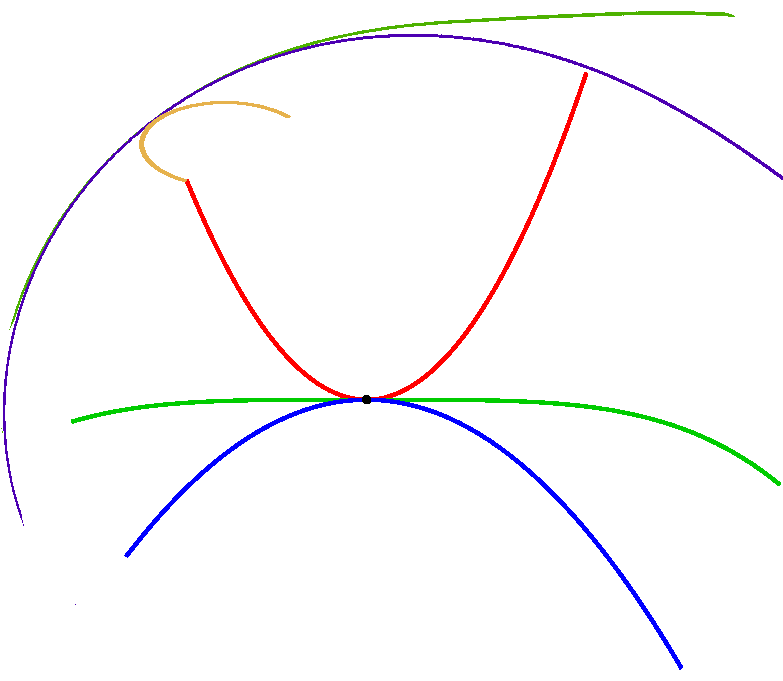
\includegraphics[width=0.8\textwidth]{part2/ruote/FIG/ruote/profili_coniugati_invil.pdf}
\end{center}
\begin{picture}(0,0)(0,0)
\scriptsize{
\put(177,110){$\eta_0$}
\put(172,116){\rotatebox{120}{$\longrightarrow$}}
\put(329,210){$\sigma_a$}
\put(312,270){$\sigma_b$}
\put(144,233){$\sigma_2$}
\put(78,64){$\lambda_{1a}$}
\put(49,119){$\lambda_{1b}$}
\put(133,160){$\lambda_2$}
}
\end{picture}
\vskip -6mm
      \caption{\em
Profili coniugati inviluppati dalla curva $\sigma_2$ trascinata dalla
polare $\lambda_2$ che rotola sia su $\lambda_{1a}$, sia su $\lambda_{1b}$.
}
 \label{fig:profili_coniugati_invil}
\end{figure}
\noindent Un caso di grande interesse, anzi, il caso che giustifica ampiamente
il procedere, che ammettiamo essere piuttosto laborioso,
di questo paragrafo, \`e quello in cui la
polare $\lambda_2$ rotola su due diverse polari:
identifichiamole coi nomi $\lambda_{1a}$ e $\lambda_{1b}$ e coi
colori verde e blu, come rappresentato
in figura \ref{fig:profili_coniugati_invil}. Anticipiamo, tanta \`e l'importanza
che attribuiamo a questo passo, che una volta ottenuti i due inviluppi, mediante
il rotolamento di $\lambda_2$ su $\lambda_{1a}$ e $\lambda_{1b}$,
sar\`a $\lambda_{1a}$ a rotolare su $\lambda_{1b}$, permettendoci cos\`i di
osservare che i due inviluppi,
precedentemente ottenuti, sono coniugati tra loro.
Le relazioni che descrivono le famiglie delle $\sigma_2$
che inviluppano $\sigma_a$ e $\sigma_b$, seguendo \ref{eq:inviluppo_polar},
saranno date dalla seguente coppia di relazioni
\begin{equation}
{\sigma_{2a}(\tau)}_\eta = 
 {\bm T}[\lambda_{1a}(\eta)]\cdot {\bm R}[\beta_{1a}(\eta)]\cdot{\bm R}[-\beta_2(\eta)]\cdot
 {\bm T} [-\lambda_2(\eta)]\cdot \sigma_2(\tau)\,,
\label{eq:inviluppo_polara}
\end{equation}
\begin{equation}
{\sigma_{2b}(\tau)}_\eta = 
 {\bm T}[\lambda_{1b}(\eta)]\cdot {\bm R}[\beta_{1b}(\eta)]\cdot{\bm R}[-\beta_2(\eta)]\cdot
 {\bm T} [-\lambda_2(\eta)]\cdot \sigma_2(\tau)\,.
\label{eq:inviluppo_polarb}
\end{equation}
\noindent Come premesso, procederemo ora in questo modo: anzich\'e fare rotolare 
la $\lambda_2$ sulle altre due primitive, facciamo rotolare la polare
$\lambda_{1a}$ sulla $\lambda_{1b}$. Il rotolamento di $\lambda_{1a}$
trasciner\`a naturalmente le
$\sigma_{2a}(\tau)_\eta$, cio\`e le curve che stanno a primo membro nella
\ref{eq:inviluppo_polara} e che definiscono l'inviluppo di $\sigma_a$.
Desideriamo dimostrare che tali curve, trascinate
dal movimento di $\lambda_{1a}$, inviluppano anch'esse la $\sigma_{b}$,
ovvero che la $\sigma_a$ inviluppa la $\sigma_b$ durante il rotolamento di 
$\lambda_{1a}$ su $\lambda_{1b}$.
Tale inviluppo sar\`a indicato con ${{\sigma_{2ab}(\tau)}_\eta}_\mu$
e, non avendo direttamente a disposizione l'espressione 
di $\sigma_a$, utilizzeremo la famiglia di curve che ne definisce l'inviluppo,
esplicitate dalla \ref{eq:inviluppo_polara}, ottenendo
\begin{multline}
{{\sigma_{2ab}(\tau)}_\eta}_\mu = 
 {\bm T}[\lambda_{1b}(\mu)]\cdot {\bm R}[\beta_{1b}(\mu)]\cdot{\bm R}[-\beta_{1a}(\mu)]\cdot
 {\bm T} [-\lambda_{1a}(\mu)]\cdot {\sigma_{2a}(\tau)}_\eta = \\
 = 
 {\bm T}[\lambda_{1b}(\mu)]\cdot\color{red} {\bm R}[\beta_{1b}(\mu)]\cdot{\bm R}[-\beta_{1a}(\mu)]\cdot
 {\bm T} [-\lambda_{1a}(\mu)]\cdot \\
\color{red} {\bm T}[\lambda_{1a}(\eta)]\cdot {\bm R}[\beta_{1a}(\eta)]\cdot{\bm R}[-\beta_2(\eta)] \color{black}\cdot
 {\bm T} [-\lambda_2(\eta)]\cdot \sigma_2(\tau)\,.
\label{eq:inviluppo_polarb1}
\end{multline}
\noindent Ricordando che le polari rotolano l'una sull'altra senza strisciare,
selezioniamo da questa doppia famiglia di curve quella di parametro
$\mu=\eta$ e componiamo le trasformazioni, scritte in colore rosso,
contenute nella \ref{eq:inviluppo_polarb1} nel seguente modo
\begin{multline}
\color{red} {\bm R}[\beta_{1b}(\eta)]\cdot{\bm R}[-\beta_{1a}(\eta)]\cdot
 {\bm T} [-\lambda_{1a}(\eta)]\cdot 
 {\bm T}[\lambda_{1a}(\eta)]\cdot {\bm R}[\beta_{1a}(\eta)]\cdot{\bm R}[-\beta_2(\eta)]=\\
={\bm R}[\beta_{1b}(\eta)]\cdot{\bm R}[-\beta_2(\eta)]\,, 
\label{eq:id}
\end{multline}
\noindent da cui si ricava immediatamente
\begin{equation}
{{\sigma_{2ab}(\tau)}_\eta}_\eta = 
 {\bm T}[\lambda_{1b}(\eta)]\cdot {\bm R}[\beta_{1b}(\eta)]\cdot
{\bm R}[-\beta_2(\eta)] \cdot
 {\bm T} [-\lambda_2(\eta)]\cdot \sigma_2(\tau)\,.
\label{eq:inviluppo_polarb2}
\end{equation}
\noindent Le espressioni del secondo membro delle \ref{eq:inviluppo_polarb2}
e \ref{eq:inviluppo_polarb} si equivalgono, pertanto
la famiglia di curve ora ottenuta coincide con quella
che si trova facendo rotolare la $\lambda_2$ sulla $\lambda_{1b}$:
${{\sigma_{2ab}(\tau)}_\eta}_\eta\equiv {\sigma_{2b}(\tau)}_\eta$,
come si evince anche dalla figura
\ref{fig:profili_coniugati_invil_lagrange}, che
rappresenta la situazione in cui la polare $\lambda_{1a}$ rotola sulla
$\lambda_{1b}$ toccandola nel punto
$\lambda_{1a}(\eta_c)\equiv \lambda_{1b}(\eta_c)$\footnote
{
Tutte le figure che rappresentano inviluppi sono state ottenute numericamente
mediante l'applicazione diretta, nel codice, delle relative formule.  Ad esempio,
la curva $\sigma_a$ di figura \ref{fig:profili_coniugati_invil_lagrange} \`e stata
ottenuta dalla implementazione numerica della relazione
\ref{eq:inviluppo_polarb2}. L'aspetto diverso di tale figura
rispetto alla precedente
\ref{fig:profili_coniugati_invil_polar}, dove sono rappresentate tutte le curve
inviluppanti, dipende dal seguente stratagemma.
Oltre alle curve che creano l'inviluppo, disegnate col colore opportuno,
viene tracciato un secondo insieme di curve, con lo stesso procedimento, in
scala leggermente minore e di
colore bianco, cio\`e quello del foglio. In tal modo si ottiene, visivamente,
il solo inviluppo. Questo artificio potrebbe essere percepito da un occhio esperto.}.
\begin{figure}[hbt]
\begin{center}
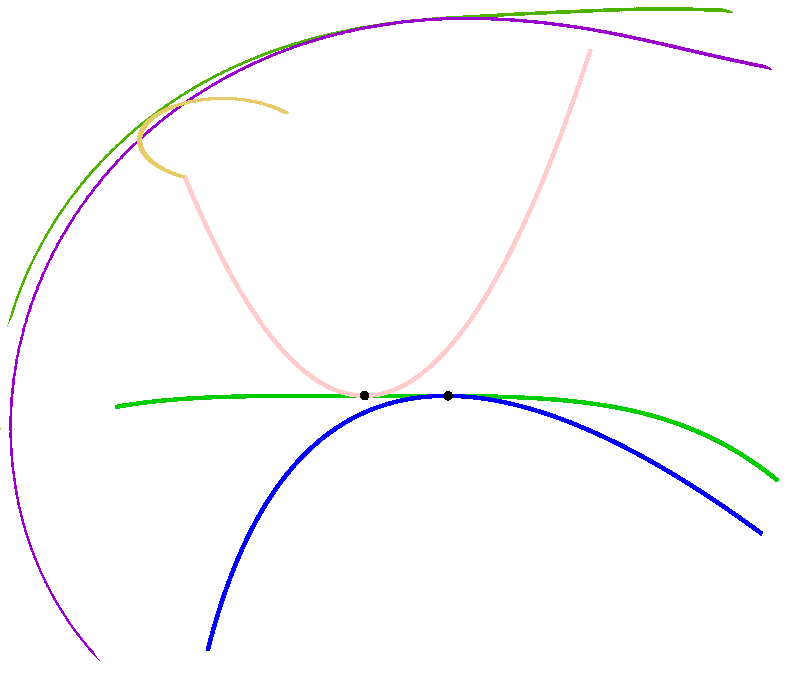
\includegraphics[width=0.8\textwidth]{part2/ruote/FIG/ruote/profili_coniugati_invil_lagrange.pdf}
\end{center}
\begin{picture}(0,0)(0,0)
\scriptsize{
\put(172,145){$\eta_0$}
\put(166,143){\rotatebox{-120}{$\longrightarrow$}}
\put(203.5,107.4){$\eta_c$}
\put(198,114){\rotatebox{120}{$\longrightarrow$}}
\put(317,242){$\sigma_a$}
\put(303,264){$\sigma_b$}
\put(142,227){$\sigma_2$}
\put(97,36){$\lambda_{1a}$}
\put(63,124){$\lambda_{1b}$}
\put(129,160){$\lambda_2$}
}
\end{picture}
\vskip -6mm
      \caption{\em
I profili $\sigma_a$ e $\sigma_b$ risultano a loro volta coniugati quando la
polare $\lambda_{1a}$ rotola sulla $\lambda_{1b}$ toccandola in $\mu_c=\eta_c$.
}
 \label{fig:profili_coniugati_invil_lagrange}
\end{figure}
\noindent Nella stessa figura sono riportate, con colori meno marcati,
anche la $\sigma_2(\tau_i)$ e la
polare $\lambda_2$ che rimangono al  proprio posto.
\noindent Possiamo quindi affermare che, dati un insieme di polari
$\lambda_i$ e un profilo $\sigma_0$
collegato ad una di queste, diciamo $\lambda_0$,
i profili coniugati $\sigma_{i}$,
che otterremo dagli inviluppi generati da $\sigma_0$ quando $\lambda_0$
rotola sull'insieme delle
$\lambda_i$\footnote{Anche se quanto affermiamo non presenta
ricadute pratiche, possiamo lasciare,
nell'insieme di polari sulle quali rotola $\lambda_0$, anche essa stessa.
 Cos\`i operando $\sigma_0$ invilupper\`a s\'e stessa.}, 
risultano tutti coniugati tra loro a coppie rispetto al moto
generato dal rotolamento delle due polari associate a ciascuna di tali
coppie.  Questo importantissimo risultato costituisce lo scopo del
presente paragrafo.
Da esso discende la possibili\`a di creare {\em profili coniugati di 
assortimento}\index{profili!di assortimento}, questione di estrema
importanza nella fabbricazione di famiglie di ruote dentate che,
a primitive date, possano ingranare l'una con l'altra.


\noindent Prendiamo di nuovo in considerazione
la trasformazione \ref{eq:inviluppo} e la figura
\ref{fig:profili_coniugati_definizione_steps}.
Se omettessimo le ultime due delle quattro trasformazioni presenti
(si parte sempre da destra), cio\`e se ci fermassimo alla parabola c),
rappresentata in azzurro chiaro,
$\sigma''_2(\tau)$,
potremmo ridisegnare la stessa figura applicando
alla $\sigma_1$, con segno opposto, le
trasformazioni non effettuate sulla $\sigma_2$. Ovviamente 
la nuova figura risulterebbe traslata verso sinistra della 
quantit\`a ${\bm T}[-\sigma_1(t)]$ e la $\sigma_1$ sarebbe
ruotata di ${\bm R}[-\alpha_1(t)]$, ma la coniugazione
tra i due profili risulterebbe perfettamente equivalente.
Pi\`u in generale, riconsiderando la famiglia di polari $\lambda_i$
e i relativi profili coniugati $\sigma_i$ possiamo scrivere,
per un dato parametro $\eta_c$,
\begin{equation}
{\sigma_i''(\tau)}_{\eta_c} = 
 {\bm R}[-\beta_i(\eta_c)]\cdot
 {\bm T} [-\lambda_i(\eta_c)]\cdot \sigma_i(\tau)\,,
\label{eq:inviluppo_polar_euler}
\end{equation}

\begin{figure}[hbt]
\begin{center}
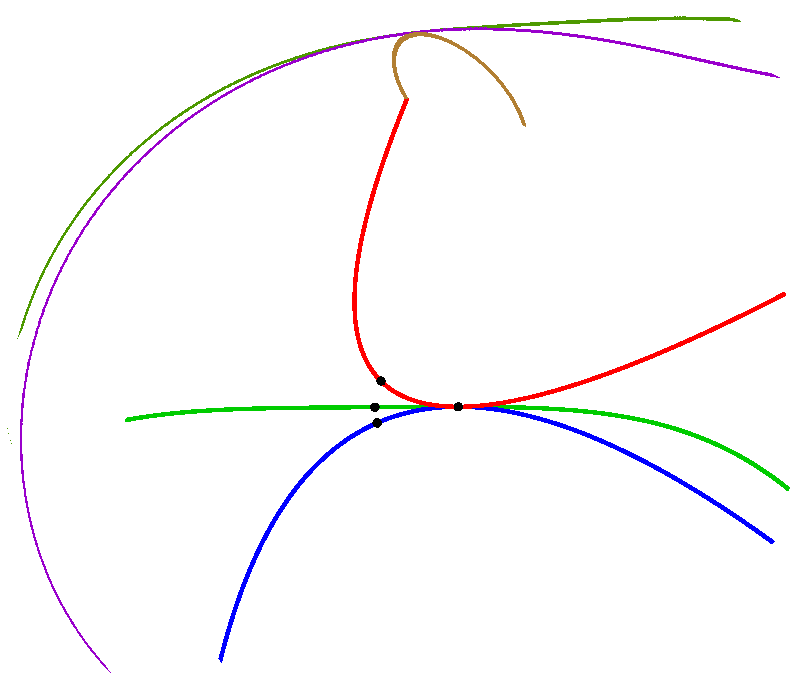
\includegraphics[width=0.8\textwidth]{part2/ruote/FIG/ruote/profili_coniugati_invil_euler.pdf}
\end{center}
\begin{picture}(0,0)(0,0)
\scriptsize{
\put(180,153){$\eta_0$}
\put(173,151){\rotatebox{-120}{$\longrightarrow$}}
\put(207,107.4){$\eta_c$}
\put(202,114){\rotatebox{120}{$\longrightarrow$}}
\put(318,244){$\sigma_a$}
\put(305,264){$\sigma_b$}
\put(222,223){$\sigma_2$}
\put(100,35){$\lambda_{1a}$}
\put(67,122){$\lambda_{1b}$}
\put(151,170){$\lambda_2$}
}
\end{picture}
\vskip -6mm
      \caption{\em
Le primitive del moto  rotolano l'una sull'altra in modo tale da mantenere
 fisso, rispetto all'osservatore assoluto, il loro punto di contatto.
}
 \label{fig:profili_coniugati_invil_euler}
\end{figure}

\noindent dove si riconosce una generalizzazione della
\ref{eq:inviluppo_polar} priva per\`o
delle ultime due trasformazioni a sinistra.
Il vantaggio offerto da questo punto di vista \`e quello di trattare
tutte le polari e i relativi profili coniugati mediante trasformazioni 
aventi la medesima struttura, le quali contengono
soltanto informazioni circa quella stessa polare o profilo coniugato.
Agendo in questo modo, il punto di contatto tra tutte le polari rimane fisso
rispetto a un osservatore assoluto e perde di senso parlare di
polari fisse e mobili. 
In figura \ref{fig:profili_coniugati_invil_euler} sono riportati
i profili coniugati e le rispettive polari, coincidenti
nei punti di parametro $\eta_c$ tramite il punto di vista
test\'e descritto e rappresentato dalla relazione \ref{eq:inviluppo_polar_euler}.
Il risultato vede ancora i profili tra loro coniugati (tutti e tre),
mentre il punto di contatto tra tutte le polari, come abbiamo
anticipato, rimane inalterato
rispetto a un osservatore assoluto. Le tre polari si muovono
in modo tale da evocare il funzionamento di un laminatoio.
In questa rappresentazione del moto relativo le polari cambiano nome
e diventano le {\em primitive del moto}\index{primitiva!del moto}.
\begin{figure}[hbt]
\begin{center}
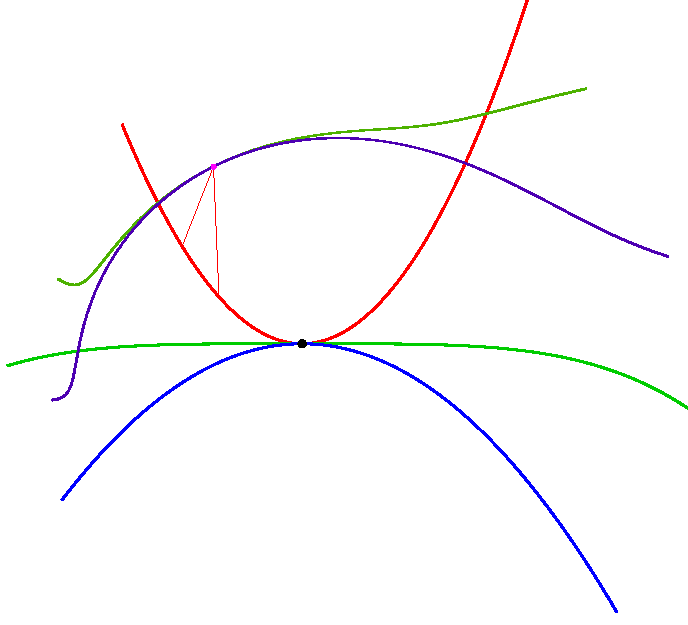
\includegraphics[width=0.8\textwidth]{part2/ruote/FIG/ruote/profili_coniugati_punto.pdf}
\end{center}
\begin{picture}(0,0)(0,0)
\scriptsize{
\put(318,180){$\sigma_a$}
\put(284,250){$\sigma_b$}
\put(124,223){$P$}
\put(48,75){$\lambda_{1a}$}
\put(25,135){$\lambda_{1b}$}
\put(84,238){$\lambda_2$}
}
\end{picture}
\vskip -6mm
      \caption{\em
Profili coniugati inviluppati come traiettorie di un punto $P$ trascinato dalla
polare $\lambda_2$ che rotola sia su $\lambda_{1a}$, sia su $\lambda_{1b}$.
}
 \label{fig:profili_coniugati_punto}
\end{figure}
\noindent Nelle figure \ref{fig:profili_coniugati_invil},
 \ref{fig:profili_coniugati_invil_lagrange} e
 \ref{fig:profili_coniugati_invil_euler} abbiamo scelto  $\sigma_2$ 
che genera gli altri profili coniugati, di forma ellittica. Se tale curva,
rimpicciolendosi, degenerasse in un punto tutto l'impianto della generazione
dei profili coniugati
rimarrebbe inalterato. Le figure
\ref{fig:profili_coniugati_punto},
\ref{fig:profili_coniugati_punto_lagrange} e
\ref{fig:profili_coniugati_punto_euler}
sono quelle che in tal caso
si ottengono. Le riportiamo
prive di commento, in quanto dovremmo ripetere i medesimi
ragionamenti che abbiamo svolto poc'anzi senza alcuna aggiunta.
Possiamo quindi affermare che anche i profili generati
come traiettoria di un punto solidale a una delle polari o primitiva del moto,
durante il suo rotolamento sulle rimanenti,
sono tra loro coniugati. 
I profili coniugati di assortimento ottenuti come inviluppo
di una linea saranno utilizzati nel prossimo paragrafo per disegnare
le ruote dentate con denti profilati a evolvente di cerchio,
le quali costituiscono la quasi totalit\`a delle ruote dentate di
uso comune nelle applicazioni tecniche.
I profili provenienti invece dalla traiettoria di un punto possono
generare ruote con denti a profilo
cicloidale. Queste, unitamente ad alcune loro applicazioni,
verranno descritte brevemente, come gi\`a segnalato, nel capitolo
\ref{ruotecy}.
A conclusione di questo laborioso paragrafo possiamo affermare
che le figure \ref{fig:profili_coniugati_invil} e
\ref{fig:profili_coniugati_punto}, insieme alle loro evoluzioni cinematiche,
sono riportate su quasi
tutti i testi di Meccanica Applicata alle Macchine. Citando il solito
\cite{sesini1}, esse si trovano tra le pagine 71 e 74. Ma tali figure
risultano reperibili in un gran numero di testi
dove campeggiano con aspetti spesso molto simili tra loro. Anche le dimostrazioni
associate, le quali assicurano la possibilit\`a di
 ottenere profili coniugati di 
assortimento, si somigliano tutte e probabilmente sono maggiormente
 valide ed eleganti, confrontate con quella che 
abbiamo proposto. Di sicuro sono molto pi\`u sintetiche.

\begin{figure}[hbt]
\centering
\begin{minipage}[b]{0.45\textwidth}
\centering
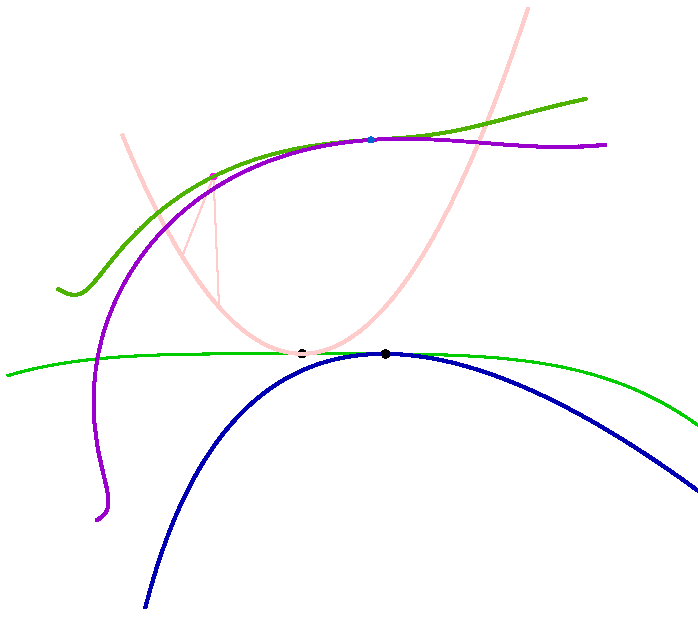
\includegraphics[width=0.9\textwidth]{part2/ruote/FIG/ruote/profili_coniugati_punto_lagrange.pdf}
\begin{picture}(0,0)(170,12)
\scriptsize{
\put(88,87){$\eta_0$}
\put(82,85){\rotatebox{-120}{$\longrightarrow$}}
\put(106,54){$\eta_c$}
\put(101,59){\rotatebox{120}{$\longrightarrow$}}
\put(150,114){$\sigma_a$}
\put(145,124){$\sigma_b$}
\put(60,113){$P_0$}
\put(94,120){$P_c$}
\put(25,35){$\lambda_{1a}$}
\put(9,67){$\lambda_{1b}$}
\put(43,118){$\lambda_2$}
}
\end{picture}
      \caption{\em
I profili $\sigma_a$ e $\sigma_b$ risultano a loro volta coniugati quando la
polare $\lambda_{1a}$ rotola sulla $\lambda_{1b}$ toccandola in un
punto con parametro $\mu=\eta=c$.
}
 \label{fig:profili_coniugati_punto_lagrange}
\end{minipage}\hfill
\begin{minipage}[b]{0.45\textwidth}
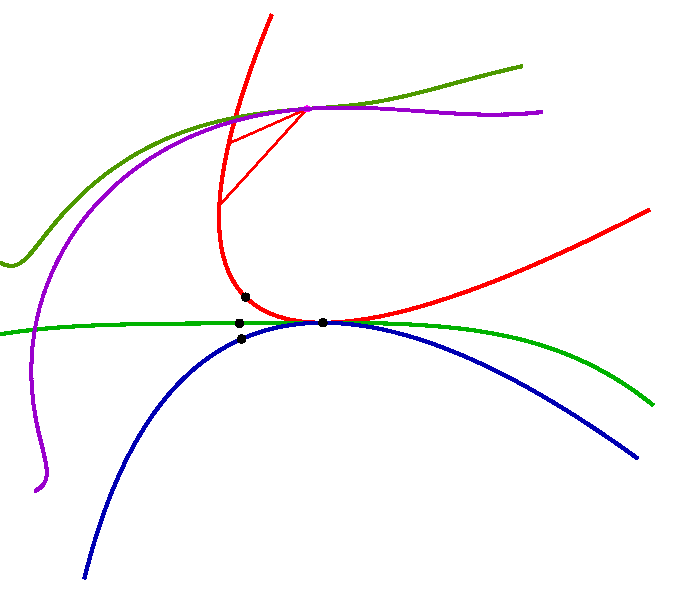
\includegraphics[width=0.9\textwidth]{part2/ruote/FIG/ruote/profili_coniugati_punto_euler.pdf}
\begin{picture}(0,0)(180,10)
\scriptsize{
\put(88,92){$\eta_0$}
\put(82,90){\rotatebox{-120}{$\longrightarrow$}}
\put(105,54){$\eta_c$}
\put(100,59){\rotatebox{120}{$\longrightarrow$}}
\put(150,115){$\sigma_a$}
\put(145,126){$\sigma_b$}
\put(94,121){$P_c$}
\put(20,33){$\lambda_{1a}$}
\put(14,67){$\lambda_{1b}$}
\put(84,140){$\lambda_2$}
}
\end{picture}
      \caption{\em
Le primitive del moto  rotolano l'una sull'altra in modo tale da mantenere
 fisso, rispetto all'osservatore assoluto, il loro punto di contatto.
      }
 \label{fig:profili_coniugati_punto_euler}
\end{minipage}
\end{figure}



\section{Profili Coniugati a Evolvente}

\noindent Torniamo ora volentieri
al percorso intrapreso, dal quale qualche perplessit\`a di troppo ci
aveva costretto a una deviazione,
per andare dritti allo studio della cinematica
delle ruote dentate.
\begin{figure}[b]
\centering
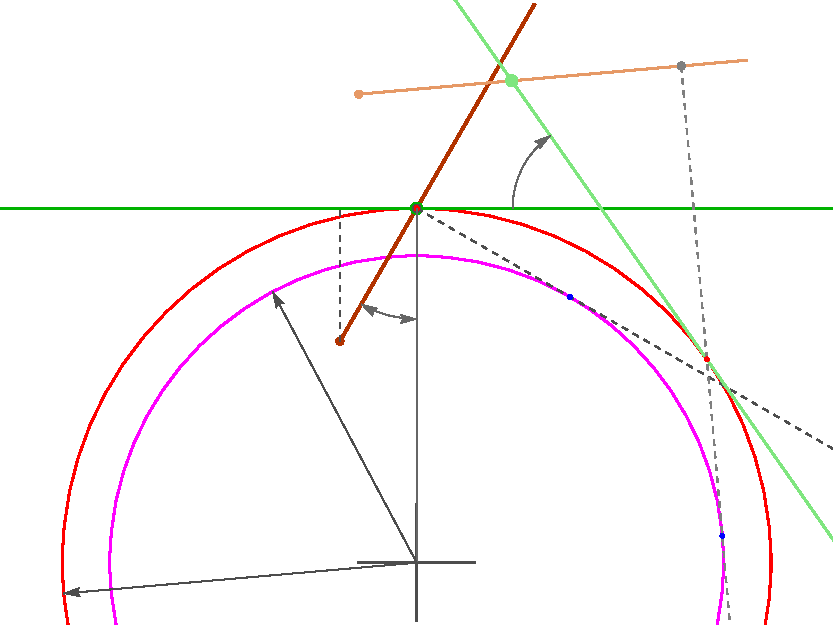
\includegraphics[width=0.8\textwidth]{part2/ruote/FIG/ruote/evol1.pdf}
\begin{picture}(0,0)(150,0)
\scriptsize{
\put(42,217){$\sigma_2$}
\put(90,198){$T'$}
\put(117,195){$\sigma'_2$}
\put(36,192){$P'$}
\put(88,160){$\mu'$}
\put(23,156){$\alpha=\alpha'$}
\put(-41,148){$P\equiv T\equiv M$}
\put(148,143){$\lambda_2$}
\put(54,119){$H$}
\put(-32,110){$h$}
\put(-12,100){$\theta$}
\put(-30,90){$F$}
\put(-28,183){$F'$}
\put(104,94){$M'$}
\put(-30,63){$r_b$}
\put(147,59){$\mu$}
\put(-55,19){$r$}
\put(146,26){$\lambda'_2$}
\put(110,29){$H'$}
\put(4,13){$O$}
\put(120,-7){$\lambda_1$}
}
\end{picture}
\vskip 3mm
      \caption{\em
Impianto geometrico per la costruzione dell'evolvente (i).
}
 \label{fig:evol1}
\end{figure}
Abbiamo lasciato il sentiero quando i dubbi circa
la bont\`a delle soluzioni che ci proponeva via via
 l'intuito hanno avvolto un punto
chiave: le ruote delle due famiglie, a) e b), rappresentate nelle figure
\ref{fig:squalo} e \ref{fig:squalo_interno}, di colore azzurro, ingraneranno
tra loro correttamente? Le notizie contenute nel precedente paragrafo ci
assicurano che i profili dei denti delle ruote a),
 ottenuti dall'inviluppo di quelli della dentatrice di figura \ref{fig:squalo}
e quelli dei denti delle b), creati invece dalla dentatrice a curvatura
opposta di figura \ref{fig:squalo_interno}, sono tutti tra loro coniugati.
Del resto, essi sono ottenuti come inviluppo di un segmento di retta
(un fianco del dente della dentatrice) che viene
trascinato dalla stessa primitiva mentre rotola sia su una 
primitiva qualsiasi delle ruote a) sia su una appartenente alle  b), inviluppando cos\`i i profili dei loro denti.
Tutte le ruote a) saranno pertanto
ingranabili con le b), con l'ovvio limite, del quale abbiamo gi\`a
fatto cenno in precedenza, che
la dimensione di queste ultime non pu\`o superare quella della ruota 
dentatrice. Tale limite ci spinge a considerare, per il diametro
della ruota di colore rosa di figura \ref{fig:squalo}, valori molto grandi:
e se pensassimo a una dentatrice di diametro infinito? In questo modo, oltre
il problema di dentare le ruote b) di grandi dimensioni, si risolverebbe
felicemente, come vedremo a breve,
 anche la noiosa questione delle due famiglie. Ricordiamo che,
a suo tempo, tra i vari precetti da rispettare nella costruzione delle ruote
dentate era emerso, in forma debole, quello di avere una sola famiglia
di ruote di assortimento.
Ci si rende facilmente conto che,
trasformando la dentatrice in una 
{\em cremagliera}\index{cremagliera}, con denti a fianco rettilineo,
tale precetto viene automaticamente
rispettato. Infatti, una circonferenza di raggio infinito presenta
curvatura pari a zero e, stante il profilo rettilineo dei suoi denti,
la dentatrice con curvatura opposta risulterebbe essere
sempre la cremagliera di partenza. Tale caratteristica \`e conosciuta
come {\em auto-complementarit\`a}\index{auto-complementarit\`a}
(dell'utensile).
Ma andiamo per gradi e consideriamo la figura \ref{fig:evol1}.
Sia $\lambda_1$ la primitiva circolare di raggio $r$ della ruota che
desideriamo costruire.
Su di essa facciamo rotolare, rigorosamente in assenza di strisciamento,
la primitiva $\lambda_2$, che \`e la retta disegnata in verde,
alla quale \`e solidale la
``curva'' $\sigma_2$, il segmento marrone inclinato di $\theta$
rispetto ad una retta ortogonale a $\lambda_2$\footnote{
La primitiva $\lambda_2$, indicata qui seguendo la tradizione come una
retta, sar\`a, per ovvie motivazioni tecniche, un segmento di lunghezza opportuna,
sufficiente ad ottenere il tratto di inviluppo che former\`a il fianco
del dente. Il segmento $\sigma_2$ viene tradizionalmente trattato come una
semiretta la quale partendo dall'estremo $F$
si estende all'infinito, permettendo in questo modo di disegnare l'intera
evolvente. Anche in questo caso ci accontentiamo di un segmento, avendo gi\`a in mente
che esso costituir\`a il fianco dei denti dell'utensile creatore.}:
questo segmento, trascinato dalla primitiva $\lambda_2$ mentre
rotola sulla circonferenza $\lambda_1$, 
creer\`a l'inviluppo che stiamo cercando.
La figura stabilisce che, per un valore dell'angolo
 $\alpha =0$, la retta  $\lambda_2$
si trovi in posizione orizzontale e sia tangente alla
 circonferenza primitiva $\lambda_1$ nel
punto $P$.
 Il processo di inviluppo, dal quale si otterr\`a il profilo coniugato
a $\sigma_2$, consta nel fare appunto rotolare la $\lambda_2$ sulla $\lambda_1$.
A una rotazione generica $\alpha=\alpha'$ corrisponderanno
la retta $\lambda'_2$ e il segmento
$\sigma'_2$.
\`E interessante individuare, su tale segmento, il punto
attivo nella creazione del profilo coniugato, cio\`e il punto $T'$
in cui il segmento
risulter\`a tangente all'inviluppo che stiamo creando.
$T'$ sar\`a perci\`o determinato
dalla intersezione della retta che, passando dal centro istantaneo di rotazione
$M'$, taglia ortogonalmente il segmento $\sigma'_2$, imponendo cos\`i che $T'$
possieda velocit\`a
parallela al segmento $\sigma'_2$ stesso.
L'individuazione di tale punto porta con s\'e
conseguenze profonde. I due triangoli $ \triangle{P' T' M'}$ e
 $\triangle{M'H'O}$
sono simili, pertanto il secondo, al di l\`a della
sua posizione, rimane lo stesso per ogni valore di $\alpha$.
Ci\`o significa che la lunghezza del segmento $(H'M')$ (indicheremo d'ora in poi
la lunghezza dei segmenti tramite le lettere che li individuano poste tra
parentesi tonde) risulter\`a
costante al variare di $\alpha$ e precisamente avremo $(H'M')= r\sin(\theta)$.
La retta $\mu'$ risulta perci\`o tangente alla
circonferenza di raggio $r_b= r \cos(\theta)$ per qualsiasi valore di $\alpha$,
dove $r_b$, grandezza di importanza rilevantissima, \`e il raggio della
{\em circonferenza di base}\index{circonferenza!di base}.
Inoltre, la lunghezza $(H'T')$ sar\`a data dalla quantit\`a 
$(M'T')$, variabile con $\alpha$, sommata alla quntit\`a fissa $(H'M')$.
Per  $\alpha=0$ abbiamo $P\equiv T\equiv M$
e naturalmente  $(H'M')=(HM)$. 
Si osserva che risulta
sempre  $(M'T')=(M'P')\cos(\theta)$ quindi, dato il rotolamento di $\lambda_2$ 
su $\lambda_1$, $(M'P')=r\alpha$ e $(M'T')=r\alpha\cos(\theta)=r_b \alpha$.
Questo indica altres\`i
che la lunghezza dell'arco $H'H$,  che sottende un angolo pari ad $\alpha$,
equivale a
$(M'T')$ e che il segmento $H'T'$ della retta $\mu'$ si comporta, al variare di
$\alpha$, come un filo che si svolge dalla circonferenza di base.

\begin{figure}[hbt] 
\centering
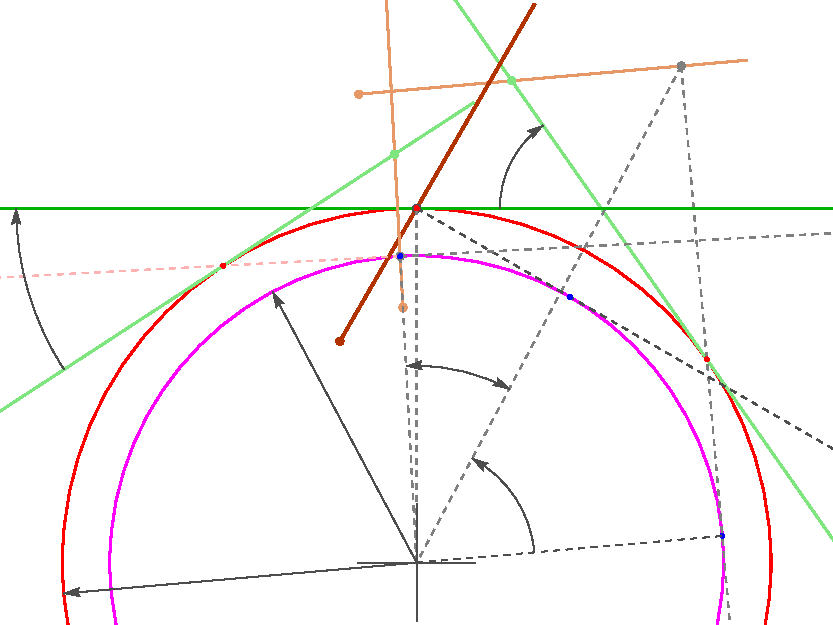
\includegraphics[width=0.8\textwidth]{part2/ruote/FIG/ruote/evol2.pdf}
\begin{picture}(0,0)(150,0)
\scriptsize{
\put(-11,218){$\sigma_2^o$}
\put(74,218){$\lambda_2^o$}
\put(42,217){$\sigma_2$}
%\put(-86,212){$P''$}
\put(90,198){$T'$}
\put(118,195){$\sigma'_2$}
\put(27,179){$P'$}
%\put(-58,181){$\sigma''_2$}
\put(88,160){$\mu'$}
%\put(-96,165){$\lambda''_2$}
\put(-2,160){$P^o$}
%\put(-30,160){$T''$}
\put(31,165){$\alpha$}
\put(6,147){$P\equiv T\equiv M$}
\put(148,143){$\lambda_2$}
\put(148,134){$\mu^o$}
\put(-76,127){$M^o$}
\put(-3,118){$T^o\equiv H^o$}
\put(56,116){$H$}
\put(-184,107){$\alpha^o=-\tan(\theta)$}
%\put(-2.2,105.5){$\delta$}
\put(104,95){$M'$}
\put(13,92){$\gamma$}
%\put(-79,83){$H''$}
\put(-30,63){$r_b$}
\put(147,59){$\mu$}
\put(34,50){$\beta$}
%\put(-133,42){$M''$}
\put(110,29){$H'$}
\put(146,26){$\lambda'_2$}
\put(-55,19){$r$}
\put(120,-7){$\lambda_1$}
%\put(-144,10){$\mu''$}
\put(4,13){$O$}
\put(-30,90){$F$}
\put(-28,183){$F'$}
\put(-13,102){$F^o$}
%
}
\end{picture}
      \caption{\em
Impianto geometrico per la costruzione dell'evolvente (ii).
      }
 \label{fig:evol2}
\end{figure}

\noindent In questo intreccio di angoli, rette e segmenti riteniamo opportuno,
riferendoci ora alla figura \ref{fig:evol2},
individuare il valore dell'angolo $\beta$ dato un generico valore di $\alpha$.
Da semplici considerazioni trigonometriche otteniamo subito
\begin{equation}
\tan(\beta) = \frac{(H'T')}{(OH')}=\
\frac{(H'M')+(M'T')}{(OH')}=\
\frac{r\sin(\theta)+\alpha  r\cos(\theta)}{r\cos(\theta)}=\
\tan(\theta) + \alpha\,.
\label{eq:beta}
\end{equation}
\vskip 1mm
\noindent Il capo del filo che si svolge dalla circonferenza di base
si individua ponendo $(H^oT^o)=0$, ottenendo in questo modo anche
il valore dell'angolo $\alpha^o$,
tale da fare coincidere $H^o\equiv T^o$:
$r\sin(\theta)+\alpha  r\cos(\theta) = 0 \rightarrow \alpha^o= -\tan(\theta)$.
Consideriamo ora la lunghezza del filo svolto dalla posizione $H^o$ alla
posizione $H'$, la lunghezza dell'arco $H'H^o$ sar\`a
\begin{equation}
\overset{\large\frown}{(H'H^o)} = (H'T') \rightarrow (\beta + \gamma) r_b= r_b \tan(\beta)\,,
\label{eq:gamma0}
\end{equation}
\noindent ottenendo pertanto
\begin{equation}
 \gamma(\beta) = \tan(\beta)-\beta \,.
\label{eq:gamma}
\end{equation}
\noindent La quantit\`a ora ricavata, unitamente alla distanza
\begin{equation}
\rho(\beta) = (OT') =  \frac{r_b}{\cos(\beta)}\,,
\label{eq:rho}
\end{equation}
\noindent forma la coppia delle coordinate polari del  punto generico
 $T'$ dell'inviluppo
che risulta essere l'{\em evolvente}\index{evolvente}
 della circonferenza di base con inizio
nel punto $H^o$. Questa curva \`e riportata in vari manuali di Matematica,
e pu\`o essere definita proprio come luogo dei punti dell'estremo di un filo
che si svolge da una determinata circonferenza a partire da un punto iniziale.
L'angolo $\beta$ riveste i panni di
parametro delle
coordinate polari di questa curva ed \`e
legato al nostro angolo di rotolamento
$\alpha$ dalla relazione \ref{eq:beta}. Tale formula permetterebbe,
invertendo la tangente, di sostituire $\beta$ con $\alpha$ nelle
\ref{eq:gamma} e \ref{eq:rho}.
Ma questa operazione
non viene in genere eseguita, forse perch\'e, come vedremo a breve,
in quel poco (o molto) utilizzo che si fa delle coordinate polari dell'evolvente,
l'angolo $\beta$ si comporta egregiamente.

\noindent Riepiloghiamo. La costruzione di profili di assortimento per i denti
ci porta a una primitiva comune a tutti gli inviluppi
che \`e una retta, $\lambda_2$, che rotoler\`a sulle primitive delle ruote da
tagliare.  Ulteriori 
considerazioni, legate alla simmetria, ci indicano come curva inviluppante
un segmento di retta, $\sigma_2$, solidale a $\lambda_2$ e inclinato
rispetto a questa di un angolo opportuno, $\pi/2 -\theta$. L'angolo $\alpha$,
mediante il quale la $\lambda_2$ rotola sulla circonferenza di raggio
$r$, governa il processo di inviluppo. Tramite i ragionamenti sopra esposti
perveniamo alla definizione di tale inviluppo che risulta essere
un'evolvente della circonferenza di base, di raggio $r_b=r \cos(\theta)$.
Pur riconoscendo l'elevato valore culturale 
di questa scoperta, del fatto cio\`e che il profilo dei denti, ottenuti tramite
il taglio con una dentiera rettilinea a fianchi pure rettilinei, sia un'evolvente
della circonferenza
di base, non dedicheremo nel presente lavoro molto spazio a questa affascinante
curva geometrica. Come riportato in \cite{guiggiani},
dal quale confessiamo di avere preso diversi spunti: ``Il fatto che il
profilo attivo sia una evolvente di cerchio \`e, in fondo, una fortunata
coincidenza''.
Ci troviamo d'accordo con questa affermazione, riservandoci
 di valutare meglio l'epiteto. Torneremo a breve
su alcune (poche) applicazioni delle formule relative all'evolvente,
nel paragrafo che tratta la correzione delle ruote mediante lo spostamento
dei profili, in particolare quando opereremo con variazione di interasse.
\noindent Prima di passare agli inviluppi veri e propri, che definiranno
la forma dei denti, \`e bene fare ancora qualche considerazione sulla
figura \ref{fig:evol2}. Quando la retta $\lambda_2$ si trova nella
posizione $\lambda^o_2$ il punto $T^o\equiv H^o$ cade sulla circonferenza
di base. Tale posizione rappresenta, sul segmento $\sigma_2$,
l'estremo oltre il quale quest'ultimo risulta inefficace nel creare
l'inviluppo. Pertanto, una posizione dell'estremo $F$ esterna a tale punto,
come quella riportata nelle  nostre figure, \`e  disutile
 in quanto la frazione in eccesso, non partecipando all'inviluppo, avrebbe come
unico effetto quello di distruggere una porzione 
del materiale da tagliare: una situazione analoga a quella
di figura \ref{fig:profili_coniugati_definizione_c}, innocua nella teoria,
inaccettabile nella pratica. La distanza $(T^oP^o)$ ha perci\`o
un significato tecnico importante e vale
\begin{equation}
(T^oP^o)=\frac{r }{\cos(\theta)}\sin^2(\theta)\,,
\label{eq:maxt}
\end{equation}
come si deduce facilmente considerando i due triangoli simili
$\triangle{OP^oM^o}$ e $\triangle{M^oP^oT^o}$.
In figura \ref{fig:evol1} \`e stata indicata con $h$ la lunghezza della
proiezione di $FP$ su una direzione ortogonale all'epiciclo $\lambda_2$. Tale
lunghezza rappresenta, come vedremo a breve, una porzione
dell'altezza dei denti dell'utensile che stiamo cercando. 

\begin{figure}[hbt] 
\centering
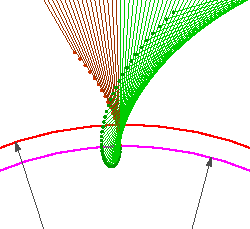
\includegraphics[width=0.7\textwidth]{part2/ruote/FIG/ruote/inviluppo_evolvente.pdf}
\begin{picture}(0,0)(150,0)
\scriptsize{
\put(14,234){$\sigma_2^o$}
\put(17,75){$T^o\equiv H^o$}
\put(-66,19){$r$}
\put(84,19){$r_b$}
\put(150,81){$\lambda_1$}
%
}
\end{picture}
      \caption{\em
Inviluppo dell'evolvente e relativo arco di trocoide. Sporgenza di $\sigma_2$
uguale ad $h_{\rm max}$, $\theta=20^{\circ}$.
      }
 \label{fig:inviluppo_evolvente}
\end{figure}
\noindent Risulta perci\`o ancora pi\`u rilevante
specificare la lunghezza della proiezione di $(T^oP^o)$ sulla direzione
ortogonale a $\lambda^o_2$, che fornir\`a
la massima altezza utile, a partire da $\lambda_2$,
dei denti della nostra dentiera generatrice:
\begin{equation}
h_{\rm max}=r  \sin^2(\theta)\,.
\label{eq:maxh}
\end{equation}
\noindent La figura \ref{fig:inviluppo_evolvente} mostra un fianco di dente,
inviluppato dal segmento $\sigma_2$, proprio in questa condizione limite,
quando cio\`e $(FP)=(T^oP^o)$.
Si pu\`o notare che, affinch\'e l'evolvente sia completa, partendo dalla
circonferenza di base, il fianco della dentiera scava ulteriormente
al di sotto di questa, costruendo un raccordo alla base del fianco del dente 
stesso. La medesima figura ci mostra che, al
variare di $\alpha$, l'estremo del segmento generatore non sconfina mai
al di l\`a del prolungamento ideale di $\sigma_2^o$ verso il centro della ruota,
essendo $\sigma_2^o$ l'ultima posizione utile nell'inviluppo dell'evolvente
stessa. Le ulteriori posizioni di $\sigma_2$, riportate in colore marrone,
rappresentano l'uscita di scena del profilo creatore. Sull'estremo inferiore
di quest'ultimo abbiamo evidenziato un minuscolo cerchio, rispettando la coerenza
del suo colore e quello del segmento che lo porta. Tali cerchi definiscono graficamente
l'arco di {\em trocoide}\index{trocoide}\footnote{
Si chiamano trocoidi le curve disegnate da punti esterni all'epiciclo
e solidali con esso durante il
rotolamento di quest'ultimo sulla circonferenza che percorre. Nel nostro caso
l'epiciclo (o ipociclo: nella teoria \`e possibile far rotolare circonferenze
pi\`u grandi all'interno di quelle pi\`u piccole) 
\`e la retta $\lambda_2$ che rotola sulla primitiva $\lambda_1$.
} che, come si vede, delinea un raccordo del profilo del dente con una
possibile circonferenza interna a quella di base: la {\em circonferenza
di piede}\index{circonferenza!di piede}.

\begin{figure}[h]
\centering
\begin{minipage}[b]{0.45\textwidth}
\centering
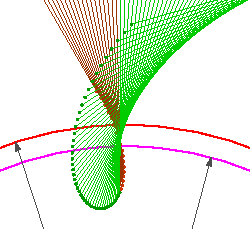
\includegraphics[width=0.9\textwidth]{part2/ruote/FIG/ruote/inviluppo_evolvente_sottotaglio.pdf}
\begin{picture}(0,0)(130,0)
\scriptsize{
\put(49.2,137){$\sigma_2^o$}
%\put(52,19){$T^o$}
\put(-8,19){$r$}
\put(89,19){$r_b$}
\put(130,45){$\lambda_1$}
}
\end{picture}
      \caption{\em
Inviluppo con $\theta=20^{\circ}$ e $(FP)=2(T^oP^o)$.
}
 \label{fig:inviluppo_evolvente_sottotaglio}
\end{minipage}\hfill
\begin{minipage}[b]{0.45\textwidth}
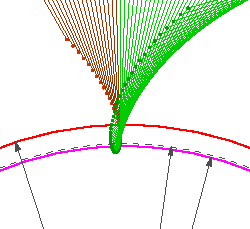
\includegraphics[width=0.9\textwidth]{part2/ruote/FIG/ruote/inviluppo_evolvente_corto.pdf}
\begin{picture}(0,0)(130,0)
\scriptsize{
\put(49.2,137){$\sigma_2^o$}
%\put(53,54){$T^o$}
\put(-8,19){$r$}
\put(89,19){$r_b$}
\put(68,19){$r_e$}
\put(130,45){$\lambda_1$}
}
\end{picture}
      \caption{\em
Inviluppo con $\theta=20^{\circ}$ e $(FP)=0.66(T^oP^o)$.
      }
 \label{fig:inviluppo_evolvente_corto}
\end{minipage}
\end{figure}

\noindent Il raggio della circonferenza di piede si deduce considerando che
la proiezione del segmento $FP$ sulla direzione ortogonale a $\lambda_2$
\`e la massima profondit\`a, in direzione radiale, alla quale arriver\`a
la trocoide e vale
\begin{equation}
r_p = r - (FP)\cos\theta = r - h\,.
\label{eq:r_p}
\end{equation}
\noindent La figura \ref{fig:inviluppo_evolvente_sottotaglio} rappresenta
l'inviluppo creato da un segmento $\sigma_2$ di lunghezza eccessiva (verso
la ruota da tagliare). L'evolvente risulta completa e tocca
la circonferenza di base, ma il fianco del dente viene scavato alla base e
una piccola parte della evolvente stessa viene distrutta: 
situazione questa che viene indicata col nome di {\em sottotaglio dei
denti}\index{sottotaglio dei denti}. 
La figura \ref{fig:inviluppo_evolvente_corto} rappresenta invece il
profilo ottenuto quando il segmento $\sigma_2$ ha una lunghezza insufficiente
a inviluppare tutta l'evolvente, alla quale mancher\`a un arco in prossimit\`a
della circonferenza di base.  La coordinata
polare radiale del punto dell'evolvente $T'$, gi\`a riportata
nella formula \ref{eq:rho}, si pu\`o anche ricavare, 
con riferimento alla figura  \ref{fig:evol2}, applicando
il teorema di Pitagora al triangolo $\triangle OT'H'$. 
Al fine quindi di individuare il raggio della circonferenza da cui partir\`a
l'evolvente, sostituiamo il
punto $T'$ con l'estremo di $F$ di $\sigma_2$ prestando attenzione
al segno opportuno per la porzione di segmento $PF$.
Stanti queste premesse, l'evolvente partir\`a da una circonferenza di raggio 
\begin{equation}
r_e = \sqrt{r_b^2 +\left(\frac{r_b\sin\theta}{\cos\theta}-\frac{(FP)\cos\theta}{\sin\theta}\right)^2}\,,
\label{eq:ini_evo}
\end{equation}
\noindent e in termini di sporgenza dei denti della dentiera (utensile) $h$
\begin{equation}
r_e = \sqrt{r_b^2 +\left(\frac{r_b\sin\theta}{\cos\theta}-\frac{h}{\sin\theta}\right)^2}\,.
\label{eq:ini_evoh}
\end{equation}

\begin{figure}[hbt]
\centering
\begin{minipage}[b]{0.45\textwidth}
\centering
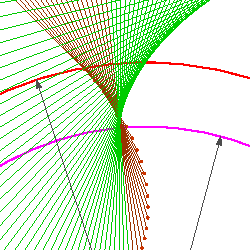
\includegraphics[width=0.9\textwidth]{part2/ruote/FIG/ruote/inviluppo_evolvente_sottotaglio35.pdf}
\begin{picture}(0,0)(130,0)
\scriptsize{
\put(43.5,150){$\sigma_2^o$}
%\put(52,19){$T^o$}
\put(20,19){$r$}
\put(88,19){$r_b$}
\put(128,98){$\lambda_1$}
}
\end{picture}
      \caption{\em
Inviluppo con $\theta=35^{\circ}$ e $(FP)=2(T^oP^o)$.
}
 \label{fig:inviluppo_evolvente_sottotaglio35}
\end{minipage}\hfill
\begin{minipage}[b]{0.45\textwidth}
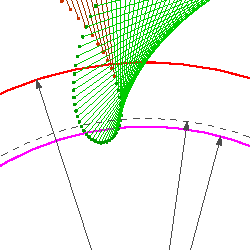
\includegraphics[width=0.9\textwidth]{part2/ruote/FIG/ruote/inviluppo_evolvente_corto35.pdf}
\begin{picture}(0,0)(130,0)
\scriptsize{
\put(43.5,150){$\sigma_2^o$}
%\put(53,54){$T^o$}
\put(20,19){$r$}
\put(88,19){$r_b$}
\put(73,19){$r_e$}
\put(128,98){$\lambda_1$}
}
\end{picture}
      \caption{\em
Inviluppo con $\theta=35^{\circ}$ e $(FP)=0.66(T^oP^o)$.
      }
 \label{fig:inviluppo_evolvente_corto35}
\end{minipage}
\end{figure}

\noindent Giusto per dare un'idea dell'influenza che il valore dell'angolo
 di pressione $\theta$ esercita su quello che sar\`a il profilo dei denti
 riportiamo le figure \ref{fig:inviluppo_evolvente_sottotaglio35} e 
\ref{fig:inviluppo_evolvente_corto35} per le quali, anzich\'e
assumere $\theta=20^{\circ}$, che \`e il valore {\em standard} dell'angolo di pressione,
si \`e posto $\theta=35^{\circ}$.
La differenza pi\`u rilevante tra queste ultime due figure e le loro precedenti
omologhe consta in una significativa riduzione del raggio di base. Ci\`o
permette, aumentando l'angolo di pressione, di poter considerare
altezze utili della dentiera pi\`u elevate, come del resto \`e evidente
anche dalla formula \ref{eq:maxh}.
Ci si pu\`o chiedere se due profili, generati con angoli $\theta$ diversi,
siano tra loro coniugati. Formulata in questo modo la domanda e di conseguenza
la risposta necessitano di qualche precisazione. La risposta \`e negativa
qualora intendessimo far rotolare,
l'una sull'altra, le due circonferenze primitive (assegnate)
e ottenere i due profili tramite due diversi epicicli.
\`E la teoria dei profili coniugati a escluderlo:
deve necessariamente essere lo stesso epiciclo a rotolare
su tutte le primitive per poter ottenere i cosiddetti {\em profili di assortimento}\index{profili!di assortimento}.
Qualora invece ci si interroghi circa la possibilit\`a di coniugare i due
profili a evolvente tramite circonferenze primitive diverse da quelle di
partenza la
risposta \`e affermativa. Infatti le due curve saranno le evolventi di 
due circonferenze di base di raggi $r_{b_1}$ e $r_{b_2}$. Se tali circonferenze
vengono affacciate, mantenendo i loro centri a distanza $i>r_{b_1}+r_{b_2}$,
si avranno due possibili raggi primitivi e un possibile angolo di pressione
dati da
\begin{equation}
r_1=\frac{r_{b_1}i}{r_{b_1}+r_{b_2}}\,,\;\;\;
r_2=\frac{r_{b_2}i}{r_{b_1}+r_{b_2}}\; {\rm e}\;\;\;
\theta=\arccos\frac{r_{b_1}+r_{b_2}}{i}\,.
\label{eq:nuove_primitive}
\end{equation}
\noindent Lasciamo la verifica di queste 
formule alla volont\`a di qualche studente.
Anticipiamo solamente che i valori dei due raggi primitivi
presentano scarso interesse applicativo, mentre quello dell'angolo di pressione
per un interasse dato risulta molto rilevante per gli ingranaggi con ruote
corrette, come vedremo, in succinto, in un prossimo paragrafo.
Il fatto che i profili a evolvente siano, entro limiti ragionevoli,
tutti fra loro potenzialmente coniugati mediante primitive circolari
risulta di grandissima importanza. Da ci\`o deriva infatti
la facolt\`a di variare, sempre entro i limiti menzionati,
 l'interasse di progetto
nella fase di montaggio delle ruote che portano tali profili:
vantaggio notevole, che permette di assorbire eventuali errori
di fabbricazione e messa in opera. Un risultato ancora pi\`u importante
della flessibilit\`a derivante dalla \ref{eq:nuove_primitive} \`e
la possibilit\`a di tagliare
le cosiddette ruote a profilo corretto nelle quali, sacrificando
senza alcun rimorso la geometria ``normale''  di tali ruote e spostando
opportunamente l'utensile creatore, si ovvia al grave problema del sottotaglio,
chiamato spesso {\em interferenza} che, come vedremo in un prossimo
paragrafo, pone un limite inferiore al numero di denti dei pignoni; ma
soprattutto offre al progettista l'opportunit\`a di individuare una strategia
di ottimizzazione degli ingranaggi, quasi sempre basata sull'utilizzo di
interassi diversi da quelli che imporrebbe il taglio di ruote ``normali''.


\section{Proporzionamento Modulare delle Ruote}

\noindent Si \`e gi\`a accennato altrove che, in ottemperanza al primo
precetto che abbiamo ammesso, cio\`e il vincolo  che impone un
numero intero di denti per le ruote dentate, nel progetto di queste ultime
si parte dal loro numero di denti, e non dai loro diametri o dai loro raggi.
Il numero di denti $z$ di una ruota rappresenta per\`o solamente una
``situazione'' geometrica angolare. In pratica, $z$ impone il
numero di spicchi mediante il quale si desidera
dividere la torta. La dimensione effettiva della
ruota deve pertanto essere legata a un fattore di scala dimensionale.
Tale parametro si chiama {\em modulo}\index{modulo}, $m$, ed \`e
a sua volta legato al numero di denti e al raggio della circonferenza primitiva
 dalla relazione
\begin{equation}
2 r =mz\,,
\label{eq:mod_z}
\end{equation}
\noindent gi\`a riportata in precedenza, ma di importanza tale da non
farci sentire in imbarazzo ripetendola. Il modulo $m$ viene espresso,
nei paesi in cui si usa il sistema metrico decimale, in ${\rm mm}$. Abbiamo 
gi\`a fatto cenno anche al {\em passo}\index{passo} della ruota che \`e
la lunghezza dell'arco di primitiva che separa due fianchi, destri o sinistri,
attigui:
\begin{equation}
p=\pi m\,.
\label{eq:passo}
\end{equation}
\noindent Dalla \ref{eq:passo} si deduce immediatamente che la possibilit\`a
di ingranare di due ruote dentate \`e condizionata dal loro modulo:
soltanto ruote con moduli uguali tra loro potranno formare ingranaggi.
L'unificazione impone per il modulo $m$ una certa successione di valori
normalizzati, della quale riportiamo i pi\`u usuali
$m=1,\;1.25,\;1.5,\;2,\;2.5,\;3,\;4,\;5,\;6\; {\rm mm}$.
Si riduce, in questo modo, la variet\`a di scelta di questo fondamentale
parametro a fronte
di notevoli vantaggi, evidenti nella fase di progettazione,
ma ancora di pi\`u se si pensa alla fase di taglio.
A ciascun valore del modulo corrisponde infatti un certo numero di utensili,
{\em in primis} la dentiera tagliente (o l'utensile creatore)
 e a seguire le mole di rettifica,
ove necessario.
Per passare dai profili rappresentati nelle precedenti figure
agli effettivi fianchi dei denti delle ruote da
tagliare occorre estendere l'impianto teorico della primitiva $\lambda_2$
equipaggiata di un solo segmento $\sigma_2$ aggiungendo altre parti e
apportando qualche leggera modifica a tali elementi.
\begin{figure}[hbt]
\begin{center}
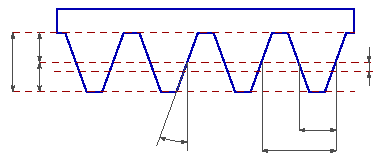
\includegraphics[width=0.94\textwidth]{part2/ruote/FIG/ruote/dentiera_riferimento.pdf}
\end{center}
\begin{picture}(0,0)(0,9.6)
\scriptsize{
\put(15,110){\rotatebox{90}{$2.5\, m$}}
\put(38,120.5){\rotatebox{90}{$1.25\, m$}}
\put(38,95){\rotatebox{90}{$1.25\, m$}}
\put(167,52){$\theta$}
\put(170,86){$F$}
\put(267,43){$p=\pi m$}
\put(264,123){$\lambda_2$}
\put(264,113.5){$\lambda_t$}
\put(76,135){$\sigma_2^-$}
\put(143,135){$\sigma_2^-$}
\put(210,135){$\sigma_2^-$}
\put(277,135){$\sigma_2^-$}
\put(121,135){$\sigma_2$}
\put(188,135){$\bm \sigma_2$}
\put(255,135){$\sigma_2$}
\put(322,135){$\sigma_2$}
\put(293,62){$p/2$}
\put(332,114){$c=mx$}
}
\end{picture}
\vskip -10mm
      \caption{\em
Dentiera normalizzata di riferimento.\index{dentiera!di riferimento}
}
 \label{fig:dentiera_riferimento}
\end{figure}

\noindent In figura \ref{fig:dentiera_riferimento} si possono notare
 la primitiva $\lambda_2$ e il segmento $\sigma_2$ contornati da
 altri oggetti
dei quali definiremo, in breve, natura e scopo.
Innanzitutto, notiamo che, a parte il numero
 di denti dell'utensile\footnote{
Il numero di denti $z_c$ dell'utensile creatore ({\em Maag}) \`e normalmente contenuto
tra i limiti $1\le z_c \le 8$, riservando il valore maggiore,
in generale, al taglio di ruote con numero di denti $z>60$.
}
e l'angolo $\theta$, tutte
le altre grandezze sono facilmente rapportabili al modulo $m$.
Il profilo $\sigma_2$, che nelle figure \ref{fig:evol1} e \ref{fig:evol2}
terminava in basso col punto $F$, e che veniva volutamente lasciato di
lunghezza indefinita all'altro capo, viene ora troncato in modo speculare
(non invertito)
rispetto a $\lambda_2$, sapendo gi\`a che i denti, dovendo avere altezza
finita, non beneficerebbero del prolungamento dell'evolvente oltre quella che,
con nome significativo, si chiama {\em circonferenza di testa}\index{circonferenza!di testa}.
Tale segmento viene poi ripetuto diverse volte e precisamente
il doppio del numero di denti di cui si vuole dotare l'utensile creatore.
La met\`a di tali segmenti, segnati coi nomi $\sigma_2^-$, 
\`e orientata in modo da creare un angolo
$-\theta$ con una linea perpendicolare  $\lambda_2$. Questi fianchi
dell'utensile sono necessari
per costruire, in una sola passata, entrambi i fianchi dei denti: le ruote
dentate trasmettono il moto in tutte e due le direzioni possibili e per
tali direzioni il loro comportamento deve essere equivalente\footnote{
Ricordiamo i precetti introdotti: il secondo (debole) prescrive
proprio questa simmetria. Esso viene talvolta disatteso, sia per particolari
applicazioni che richiedono asimmetria di comportamento dell'ingranaggio
rispetto alle direzioni del flusso di potenza, sia per ottenere
vantaggi circa la riduzione di rumorosit\`a della trasmissione, come 
testimoniato da alcune specifiche e recenti ricerche.
Stando alla nostra modesta esperienza,
confessiamo per\`o di non aver mai toccato con mano
 {\em ruote asimmetriche}\index{ruote!asimmetriche}.}.
Per una {\em dentiera normalizzata}\index{dentiera!normalizzata}
valgono le seguenti relazioni, una parte delle quali \`e riportata 
anche nella figura:
l'altezza dei denti \`e legata al modulo e vale $2.5\,m$, ugualmente
ripartita tra {\em addendum}\index{addendum} e {\em dedendum},\index{dedendum}
che pertanto valgono entrambi $1.25\, m$; i denti e i vani hanno la 
medesima forma e il passo tra due fianchi consecutivi e omologhi,
misurato su una
qualunque retta orizzontale che intercetti tali fianchi, vale $p=\pi m$.
Il valore dell'angolo di pressione che, in Europa, si ritiene normalizzato
vale $\theta=20^{\circ}$.
Oltre alla primitiva $\lambda_2$, sempre in figura 
\ref{fig:dentiera_riferimento}, troviamo la retta orizzontale $\lambda_t$
che chiameremo {\em primitiva di taglio}\index{primitiva!di taglio},
e che individua l'effettiva primitiva usata durante il moto di taglio:
essa, rotolando sulla primitiva della ruota da tagliare,
crea, tramite i profili $\sigma$, i profili dei denti.
Tale retta, rappresentata a distanza $c=mx$ 
da $\lambda_2$, si trover\`a a coincidere con questa ($c=0$) nel
taglio di {\em ruote normali non corrette}\index{ruote!non corrette}:
$x$ si chiama {\em fattore di correzione adimensionale}\index{correzione!adimensionale}, del quale daremo qualche ulteriore notizia in
un prossimo paragrafo.

\section{Taglio delle Ruote Dentate per Inviluppo}

\noindent Siamo ormai dotati dell'utensile opportuno per poter
eseguire di nuovo le dentature delle figure \ref{fig:squalo} e
 \ref{fig:squalo_interno}. Chiediamo al lettore di pazientare ancora
un momento, in modo da poter ritoccare il nostro utensile e renderlo somigliante
a quelli che realmente si usano nel processo industriale del taglio delle 
ruote dentate.
\noindent Chiariamo subito che la dentiera rappresentata in figura \ref{fig:dentiera_maag}
corrisponde solo teoricamente a quelle che si usano nel processo di taglio
per inviluppo delle ruote dentate e che portano il nome {\em Maag}\index{dentiera!Maag}.
\begin{figure}[t]
\begin{center}
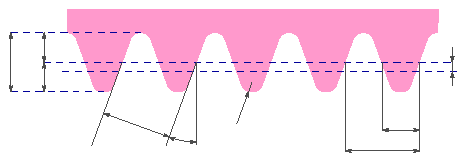
\includegraphics[width=0.98\textwidth]{part2/ruote/FIG/ruote/dentiera_maag.pdf}
\end{center}
\begin{picture}(0,0)(0,9.6)
\scriptsize{
\put(5,99){\rotatebox{90}{$2.5\, m$}}
\put(33,116){\rotatebox{90}{$=$}}
\put(33,93){\rotatebox{90}{$=$}}
\put(181,55){$r_r=0.4m$}
\put(132,36){$\theta=20^{\circ}$}
\put(90,69){\rotatebox{-20}{$p_b=p \cos\theta$}}
\put(287,42){$p=\pi m$}
\put(277,110){$\lambda_2$}
\put(277,102){$\lambda_t$}
\put(307,59){$p/2$}
\put(339,102){$c=mx$}
}
\end{picture}
\vskip -6mm
      \caption{\em
Utensile Maag.
}
\vskip -3mm
\label{fig:dentiera_maag}
\end{figure}
Infatti, tali utensili a forma di pettine
devono possedere, oltre alle qualit\`a geometriche che interessano la nostra
disciplina, molti altri accorgimenti, come quelli che permettano il loro
afferraggio sulla macchina dentatrice
e altri che facilitino il processo tecnologico del taglio mediante asportazione
di truciolo: i taglienti affilati e
gli angoli di spoglia, irrinunciabili in tali processi\footnote{
Nella pratica \`e molto frequente mettere diversi pettini come quelli di
figura \ref{fig:dentiera_maag} adagiati sulle generatrici di un cilindro, ottenendo
cos\`i quello che in gergo si chiama {\em creatore}\index{creatore}. Il creatore taglia i denti 
tramite un movimento rotatorio e traslatorio e il moto di rotolamento tra le due
primitive avviene con continuit\`a. Per quest'ultimo motivo, l'asse
dei denti di ciascun pettine deve essere un'elica, e l'insieme di queste
schiere di denti conferiscono all'utensile l'aspetto di una vite.
} e non facilmente rappresentabili nel piano dove giacciono i profili dei denti.
La differenza pi\`u evidente tra la dentiera di riferimento di figura
\ref{fig:dentiera_riferimento} e l'utensile Maag, \`e la forma arrotondata
delle teste e del fondo dei denti. Questo accorgimento si rende necessario
per due ordini di difficolt\`a che l'uso di una dentiera
con spigoli vivi comporterebbe.
La prima di tali difficolt\`a risiede in ambito tecnologico
e si pu\`o riassumere dicendo che i taglienti spigolosi (bench\'e ammissibili)
sono estremamente pi\`u fragili rispetto a quelli che presentano spigoli
arrotondati. Il secondo vantaggio offerto dallo smusso dei denti riguarda
la possibilit\`a di costruire pignoni recanti un minor numero di denti,
cio\`e di ovviare in parte a quello che tradizionalmente si
chiama {\em problema dell'interferenza}, alla soluzione del
 quale dedicheremo, appena pi\`u avanti, uno spazio adeguato.
\begin{figure}[hbt]
\centering
\begin{minipage}[b]{0.48\textwidth}
\centering
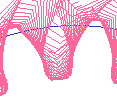
\includegraphics[width=0.98\textwidth]{part2/ruote/FIG/ruote/17denti_4mod_20gradi_0corr_0p01rr_inv.pdf}
\begin{picture}(0,0)(130,0)
\scriptsize{
\put(7,45){\rotatebox{25}{$\longrightarrow$}}
\put(9,38){\rotatebox{35}{$\longrightarrow$}}
\put(14,30){\rotatebox{45}{$\longrightarrow$}}
\put(27,21){\rotatebox{75}{$\longrightarrow$}}
\put(0,13){punti della trocoide}
}
\end{picture}
      \caption{\em
Profilo dei denti generati dalla dentiera di riferimento: $z=17$, $\theta=20^{\circ}$, $r_r=0$.
}
 \label{fig:17denti_4mod_20gradi_0corr_0p01rr_inv}
\end{minipage}\hfill
\begin{minipage}[b]{0.48\textwidth}
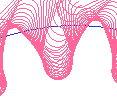
\includegraphics[width=0.98\textwidth]{part2/ruote/FIG/ruote/17denti_4mod_20gradi_0corr_0p4rr_inv.pdf}
\begin{picture}(0,0)(130,0)
\scriptsize{
}
\end{picture}
      \caption{\em
Profilo dei denti generati da dentiera {\em Maag}: $z=17$, $\theta=20^{\circ}$, $r_r=0.4m$.
      }
 \label{fig:17denti_4mod_20gradi_0corr_0p4rr_inv}
\end{minipage}
\vskip -3mm
\end{figure}
Crediamo sia istruttivo fare un confronto tra gli inviluppi
prodotti dalla dentiera di riferimento
e dall'utensile {\em Maag} sullo stesso pignone con $z=17$, che, come
vedremo, presenta il minimo numero di denti possibili, al di sotto del quale
si manifesta il sottotaglio alla base dei denti. 
Come mostrato in figura 
\ref{fig:17denti_4mod_20gradi_0corr_0p01rr_inv}, la quale riporta
l'inviluppo ottenuto da una dentatrice con spigoli vivi,
lo sconfinamento verso l'asse del dente dei
 punti del raccordo di piede (l'arco di trocoide) rende la base del 
dente stesso sottotagliata. Questo comporta una sua diminuzione della
resistenza a flessione, comportandosi il dente, dal punto di vista
strutturale, come una mensola
sollecitata da un carico collocato a distanza variabile dall'incastro.
 Del resto il sottotaglio era prevedibile in quanto,
 stando al proporzionamento modulare della dentiera di riferimento,
abbiamo per l'altezza dei suoi denti $h=1.25 m$.  Sostituendo questo valore nella
\ref{eq:maxh} otteniamo
\begin{equation}
z_{\rm min}=\frac{2.5}{\sin^2(\theta)}\,,
\label{eq:zminrif}
\end{equation}
\noindent e per $\theta= 20^{\circ}$ si  ottiene
$z_{{\rm min}_{20^{\circ}}}=22$\index{numero minimo di denti}. Gi\`a in questo luogo, desideriamo
mettere in evidenza, alla buona, cio\`e mediante il calcolo
diretto della \ref{eq:zminrif} per
$\theta=25^{\circ}$, la sensibilit\`a del risultato di
 tale formula alla variazione dell'angolo di 
pressione: abbiamo, ad esempio, $z_{{\rm min}_{25^{\circ}}}=14$. La figura
\ref{fig:17denti_4mod_20gradi_0corr_0p4rr_inv} riporta invece il
profilo dei denti di un pignone con $z=17$ e $\theta = 20^{\circ}$ ottenuto per\`o
tramite utensile {\em Maag}, a spigoli smussati, con raggio di raccordo delle creste
dei denti $r_r=0.4m$.
In quest'ultimo caso, si nota che le teste dei denti
dell'utensile sono molto vicine al limite del sottotaglio\footnote{
Quanto qui asserito ($z_{{\rm min}_{20^{\circ}}}=17$) si ricava facilmente
osservando che nella formula \ref{eq:zminrif}, nel caso di utensile con denti
 smussati, il numeratore passerebbe da $2.5$ a $2$.
},
pertanto si ammette in generale,
e nelle condizioni ora menzionate, che il numero minimo  di denti per
un pignone (senza correzione) \`e $z_{{\rm min}_{20^{\circ}}}=17$.
Nelle due figure ora citate riportiamo anche un arco della circonferenza di
testa o di troncatura della ruota da tagliare, circonferenza che delimita
l'estremit\`a esterna dei denti.
Notiamo che in questo caso
la presenza di uno smusso alla base dei denti della dentiera non
incide sulla forma della testa dei denti della ruota:
 tale raccordo \`e un mero accorgimento costruttivo,
\begin{figure}[t]
\centering
\begin{minipage}[b]{0.48\textwidth}
\centering
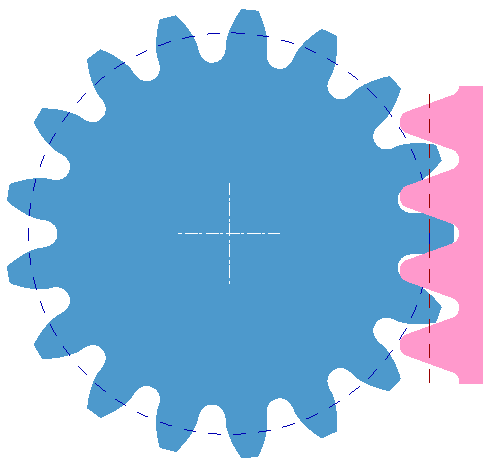
\includegraphics[width=0.98\textwidth]{part2/ruote/FIG/ruote/17denti_4mod_20gradi_0corr_0p4rr.pdf}
\vskip 5mm
\begin{picture}(0,0)(130,0)
\scriptsize{
}
\end{picture}
      \caption{\em
Pignone con $z=17$, $\theta=20^{\circ}$: assenza di sottotaglio.
}
 \label{fig:17denti}
\end{minipage}\hfill
\begin{minipage}[b]{0.48\textwidth}
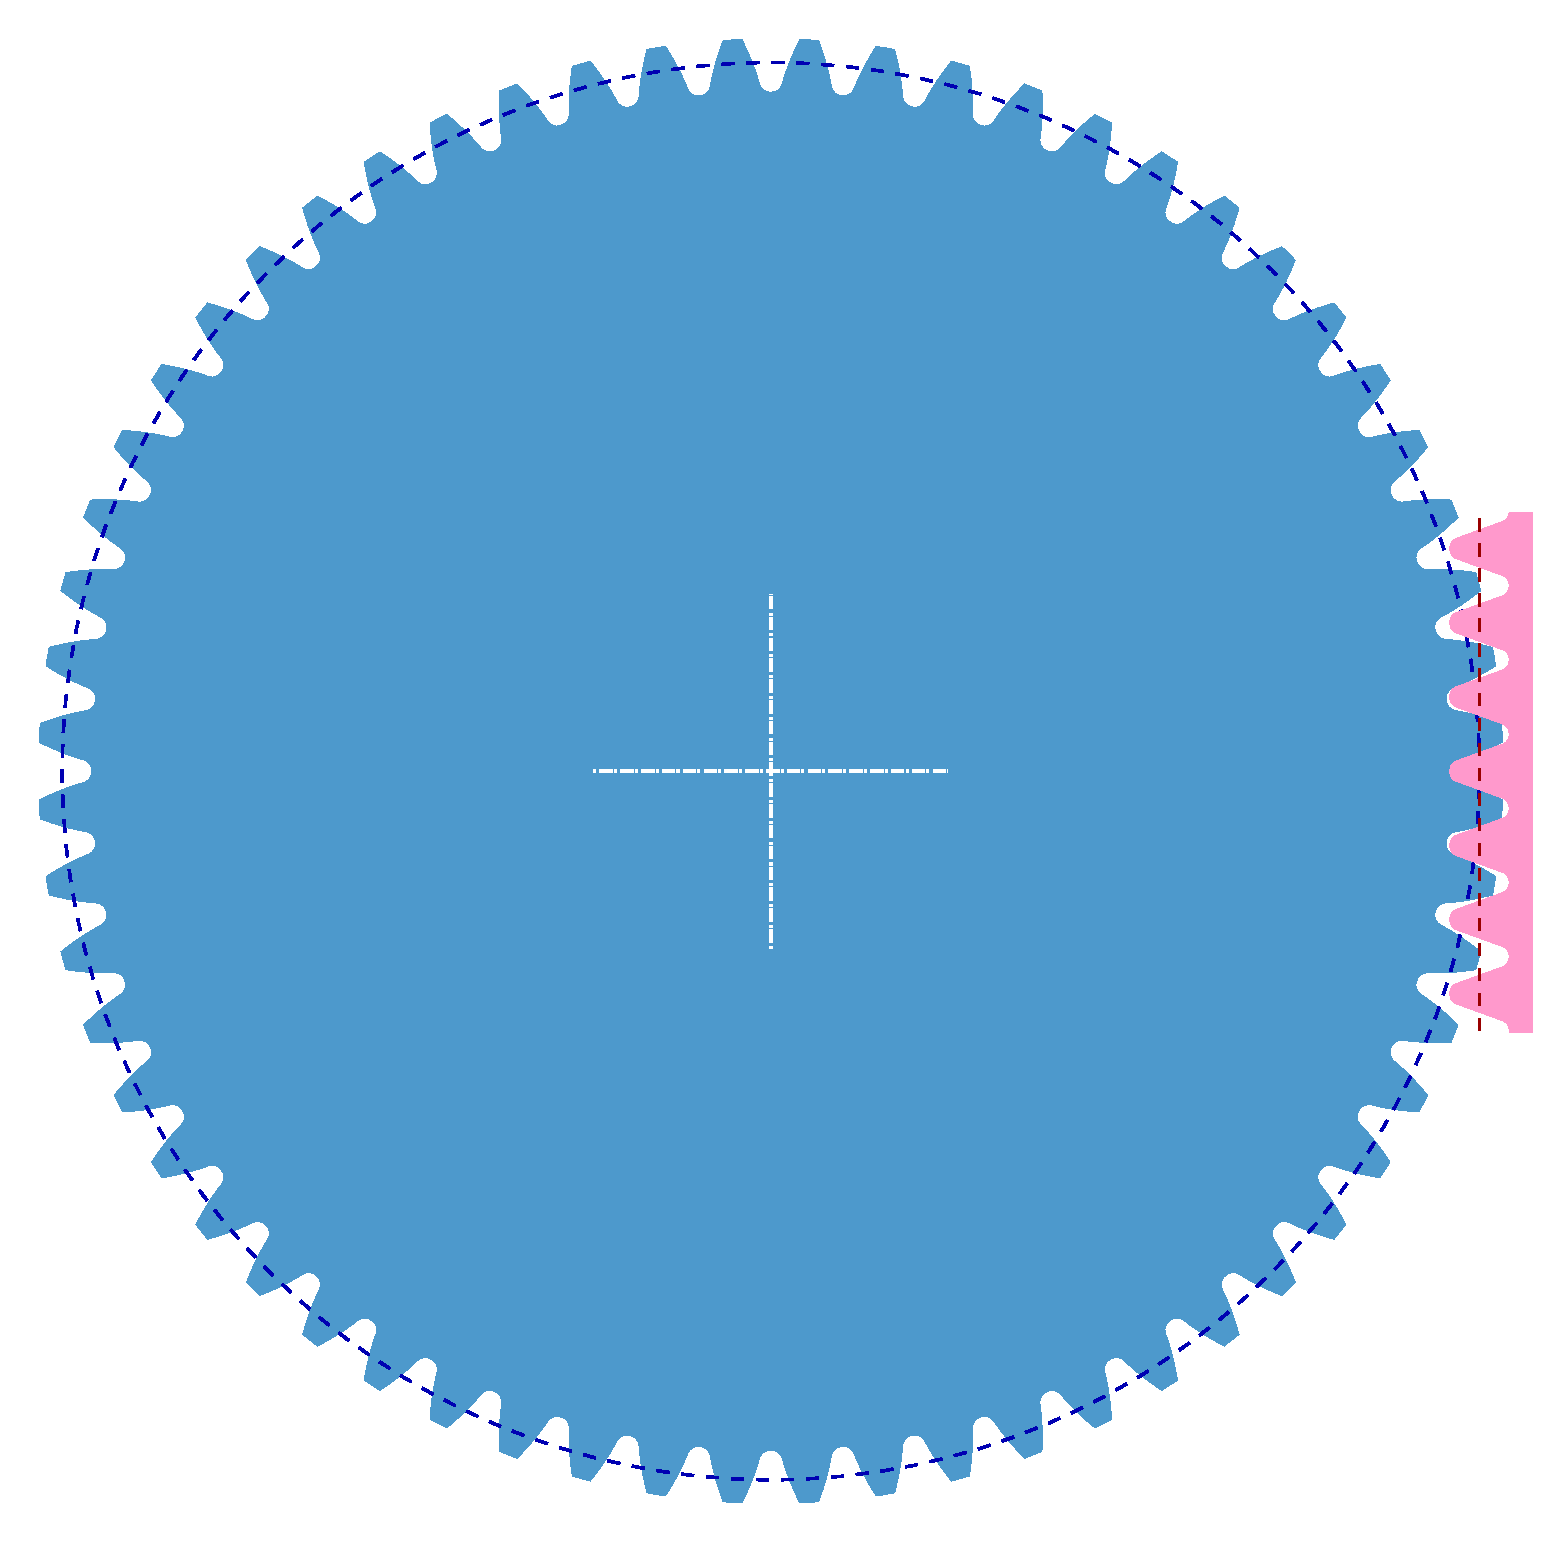
\includegraphics[width=0.98\textwidth]{part2/ruote/FIG/ruote/60denti_4mod_20gradi_0corr_0p4rr.pdf}
\begin{picture}(0,0)(130,0)
\scriptsize{
}
\end{picture}
      \caption{\em
Ruota dentata con $z=60$, $\theta=20^{\circ}$: fianchi dei denti somiglianti a quelli di una cremagliera.
      }
 \label{fig:60denti}
\end{minipage}
\vskip -3mm
\end{figure}
\noindent In figura \ref{fig:17denti} riportiamo finalmente ci\`o che si ottiene
tagliando una ruota con la dentiera {\em Maag} quando le due primitive, quella
della dentiera e quella della ruota, coincidono. Il pignone raffigurato ha
numero di denti $z=17$, angolo di pressione $\theta=20^{\circ}$
e, come si pu\`o notare visivamente,
 ci troviamo al limite del sottotaglio, anche se il numero di denti \`e
inferiore a 22 che, ripetiamo, rappresenta il minimo teorico per un
utensile con spigoli vivi.
La figura \ref{fig:60denti} mostra invece una ruota con $z=60$ e angolo
di pressione sempre $\theta=20^{\circ}$. In questo caso si nota che,
trovandoci molto lontani dal numero minimo di denti, la circostanza
del sottotaglio \`e
ben lungi dal presentarsi e i denti appaiono molto robusti alla base.
Si pu\`o osservare inoltre che i fianchi
dei denti, pur essendo (ovviamente) degli archi di evolvente,
assomigliano molto a quelli rettilinei della cremagliera.
Crediamo sia istruttivo rappresentare l'ingranamento di queste
due ruote, che naturalmente
le riconduce nella stessa scala (figura \ref{fig:1760}).

\noindent Siamo finalmente giunti alla fine del nostro percorso che, rispettando
i vincoli ``naturali'' che a mano a mano si sono palesati, ha portato a una
soluzione che appare quasi unica. Rimane ancora una verifica da effettuare,
che sottintende un precetto forte (l'ultimo): l'ingranaggio di due ruote
dentate deve essere in grado di trasmettere il moto con continuit\`a. Questo
significa che le coppie di denti a contatto devono sempre essere in numero
 maggiore
dell'unit\`a.
\begin{figure}[hbt]
\begin{center}
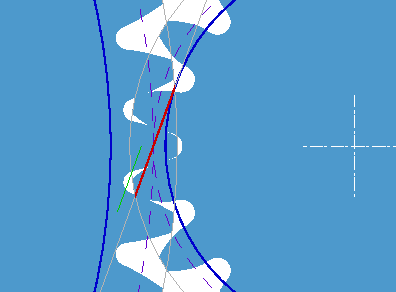
\includegraphics[width=1.0\textwidth]{part2/ruote/FIG/ruote/1760.pdf}
\begin{picture}(0,0)(200,0)
\scriptsize{
\put(180,197){$A$}
\color{white}
\put(280,160){$z_1=17$}
\put(50,160){$z_2=60$}
\put(331,139){$O_1$}
\put(151,145){$P$}
\put(134,97){$B$}
\put(122,83){$p_b$}
\put(126,73){$\mu$}
\put(100,46){$r_{b_2}$}
\color{black}
\put(146,46){$r_{p_2}$}
\put(198,31){$r_{p_1}$}
\put(216,31){$r_{b_1}$}
\put(158,23){$r_{t_2}$}
\put(181,23){$r_{t_1}$}
}
\end{picture}
\end{center}
\vskip -5mm
\caption{ \em
Ingranaggio con $z_1=17$, $z_2=60$, $\theta=20^{\circ}$.
} 
\vskip -3mm
\label{fig:1760}
\end{figure}
\noindent Con riferimento alla figura \ref{fig:1760}, ricordando che 
i punti di contatto (coniugati) tra due fianchi di evolvente giacciono
sulla perpendicolare alle evolventi stesse in tali punti, possiamo affermare
che i contatti tra i denti avvengono solo sulla retta $\mu$, tangente
alle due circonferenze di base di raggi $r_{b_1}$ e $r_{b_2}$, e chiamata
{\em retta delle pressioni}\index{retta delle pressioni}.
Pi\`u in dettaglio, le posizioni dei contatti saranno interne alle due 
circonferenze di testa delle ruote, le quali delimitano il tratto $AB$ che,
nella figura \ref{fig:1760}, \`e rappresentato in rosso. Affinch\'e
la trasmissione del moto avvenga con continuit\`a, sul segmento $AB$ devono
essere presenti uno o pi\`u punti di contatto. Sulla retta delle pressioni
i profili dei denti si succedono col passo che si misura sulle circonferenze
di base, dalle quali ``nascono'' le evolventi, destre o sinistre,
 e che naturalmente coincide con il passo della  successione dei fianchi, 
destri o sinistri, dei denti dell'utensile, misurato in direzione normale ai
fianchi stessi. Tale misura, indicata in figura \ref{fig:dentiera_maag}, vale
$p_b=\pi m \cos \theta$. Anche questa lunghezza \`e riportata in 
figura \ref{fig:1760}, giusto per
un confronto visivo, mediante un segmento verde.
Riepilogando, la trasmissione del moto sar\`a continua se il 
{\em fattore di ricoprimento}\index{fattore di ricoprimento} $f_c$, dato
dal rapporto tra la lunghezza del segmento $AB$ e il passo di base, \`e
maggiore dell'unit\`a: $f_c=(AB)/p_b>1$.
 La lunghezza del segmento $PB$ (come del resto quella del segmento
$PA$) si determina applicando il teorema del coseno al triangolo $\triangle{O_1BP}$ (oppure $\triangle{O_2AP}$). Per $(PB)$ si ha
\begin{equation}
(PB)^2  +2r_{p_1}\sin( \theta)(PB)+r_{p_1}^2 - r_{t_1}^2=0\,.
\label{eq:segpb2}
\end{equation}
\noindent Pertanto, indicando le lunghezze $(PA)$ e $(PB)$ semplicemente
con $\eta$ e togliendo i pedici che identificano una delle due ruote, possiamo 
scrivere
\begin{equation}
\eta= -r_p\sin( \theta)\pm \sqrt{r_p^2\sin^2(\theta)-r_p^2 + r_t^2}\,.
\label{eq:segpb3}
\end{equation}
\noindent Introducendo le grandezze legate al proporzionamento normale 
e facendo il rapporto tra $\eta$ e il passo base $p_b$ abbiamo
\begin{equation}
\frac{\eta}{p_b}= \frac{-(z/2)\sin( \theta)\pm \sqrt{(z/2)^2\sin^2(\theta)+ z+1}}{\pi \cos (\theta)}\,.
\label{eq:segpb3_1}
\end{equation}
\noindent La formula \ref{eq:segpb3_1} fornisce,
con  $z=17$, un fattore di ricoprimento,
nel tratto di competenza $PB$, $\underline f_c=\eta/p_b=0.75$. La qual cosa  significa
che, nel caso peggiore (ammissibile per non avere sottotaglio),
cio\`e quando l'ingranaggio \`e costituito da due pignoni da diciassette denti,
essi possono ingranare tra loro con continuit\`a essendo, in questo caso,
$f_c=1.5$.

\section{Ruote Corrette mediante Spostamento del Profilo I} \label{ruote-corr1}

Le proporzioni della dentiera di riferimento di figura
\ref{fig:dentiera_riferimento} risultano sicuramente ragionevoli ma, 
rappresentando un compromesso esteso a tutte le ruote, qualsiasi
sia il loro numero di denti e quello della ruota accoppiata,
si intuisce facilmente che esse potrebbero non rappresentare
la scelta ottimale.
\begin{figure}[b]
\begin{center}
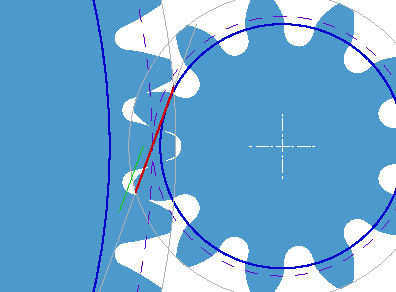
\includegraphics[width=1.0\textwidth]{part2/ruote/FIG/ruote/1160.pdf}
\begin{picture}(0,0)(200,0)
\scriptsize{
\put(180,197){$A$}
\color{white}
\put(280,155){$z_1=11$}
\put(50,155){$z_2=60$}
\put(285,138){$O_1$}
\put(151,145){$P$}
\put(123,82){$p_b$}
\put(124,71){$\mu$}
\put(99,46){$r_{b_2}$}
\color{black}
\put(135.5,103.5){$B$}
\put(146,46){$r_{p_2}$}
\put(213,44){$r_{p_1}$}
\put(224,50){$r_{b_1}$}
\put(158,23){$r_{t_2}$}
\put(190,23){$r_{t_1}$}
}
\end{picture}
\end{center}
\vskip -5mm
\caption{\em
Ingranaggio con $z_1=11$, $z_2=60$, $\theta=20^{\circ}$ senza correzioni.
} 
\vskip -3mm
\label{fig:1160}
\end{figure}
\noindent In figura \ref{fig:1160} \`e riportato l'ingranaggio di un pignone
con $z_1=11$ denti e $z_2=60$ denti. Si nota subito che i denti del pignone
si presentano scavati alla base. Ci\`o era ampiamente prevedibile in quanto
la \ref{eq:zminrif}, pur considerando l'arrotondamento dei taglienti
dell'utensile creatore, non permette di scendere sotto il numero 
$z_{\rm min}=17$, senza che il sottotaglio si manifesti. La scarnitura del
dente alla base \`e una circostanza molto grave? Certamente la resistenza
a flessione del dente stesso ne risente. E dal punto di vista della nostra
disciplina? Apparentemente, in quest'ambito, le cose vanno meglio: la cinematica
dell'ingranaggio \`e comunque corretta. Ma l'impegno dell'evolvente di cerchio
fino alla sua radice fa sorgere un'altra preoccupazione, dovuta al fatto che
in quel punto, com'\`e noto, il raggio di curvatura del profilo \`e pari a zero,
e da ci\`o possono emergere altre problematiche di carattere strutturale.
Per\`o, la grande produttivit\`a delle dentatrici di ruote a evolvente,
la relativa semplicit\`a di costruzione degli utensili necessari,
la possibilit\`a di affilare tali utensili senza compromettere la loro
forma ``operativa'' ci convincono, in un ragionamento un po' fantastico,
che il mondo della meccanica avrebbe accettato tranquillamente anche le
ruote sottotagliate qualora, a tale problema, non ci fosse stato rimedio
 e anzi, in talune applicazioni, cui faremo cenno alla
fine del prossimo paragrafo, tali ruote si accettano appunto.
Ma il rimedio esiste, ed \`e uno di quei ``toccasana'' che non comporta
spese, al contrario, oltre a determinare la scomparsa del sottotaglio,
le {\em correzioni tramite
lo spostamento del profilo}\index{correzione!profilo} portano una serie
di vantaggi tali da essere impiegate anche quando il sottotaglio non si
manifesta affatto.
In aggiunta, mentre da un punto di vista didattico le dentature
corrette presentano per lo studente un ulteriore (l'ultimo) piccolo
grattacapo, nella pratica esse si progettano e si eseguono con estrema
disinvoltura: se si dovesse progettare l'ingranaggio di figura \ref{fig:1760}
e il pignone di $z_1=17$ denti fosse la ruota motrice
ben difficilmente esso non verrebbe corretto.
\begin{figure}[hbt]
\begin{center}
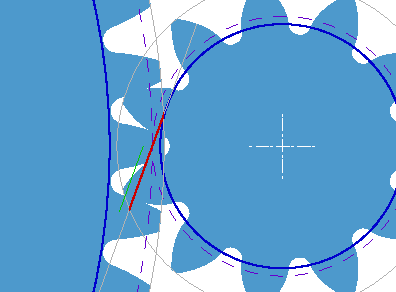
\includegraphics[width=1.0\textwidth]{part2/ruote/FIG/ruote/1160c_i0.pdf}
\begin{picture}(0,0)(200,0)
\scriptsize{
\color{white}
\put(170,172){$A$}
\put(280,155){$z_1=11$}
\put(50,155){$z_2=60$}
\put(285,138){$O_1$}
\put(148,144){$P$}
\put(123,82){$p_b$}
\put(124,71){$\mu$}
\put(97,46){$r_{b_2}$}
\put(138,86){$B$}
\color{black}
\put(146,46){$r_{p_2}$}
\put(213,38){$r_{p_1}$}
\put(225,49){$r_{b_1}$}
\put(157,23){$r_{t_2}$}
\put(190,23){$r_{t_1}$}
}
\end{picture}
\end{center}
\vskip -5mm
\caption{\em
Ingranaggio con $z_1=11$, $z_2=60$, $\theta=20^{\circ}$, con correzioni $x_1=0.5$ e $x_2=-0.5$.
} 
\vskip -3mm
\label{fig:1160c_i0}
\end{figure}
Ricordiamo che nelle due figure \ref{fig:dentiera_riferimento} e
\ref{fig:dentiera_maag} abbiamo riportato una retta tratteggiata indicata
con $\lambda_t$, chiamata {\em primitiva di taglio}\index{primitiva!di taglio}, distante dalla primitiva della
dentiera di una quantit\`a $c=m x$. Quando le ruote vengono tagliate facendo
rotolare $\lambda_t$ sulla primitiva teorica delle ruote stesse con $c \ne 0$
esse si dicono {\em corrette}\index{ruote!corrette}. Riferendoci all'utensile {\em Maag} (ma
la questione rimane identica anche per utensili creatori a vite), si tratta
semplicemente di spostare la dentiera di una quantit\`a $c$ verso l'esterno
della ruota da
tagliare se $c >0$, oppure verso l'interno qualora la correzione fosse negativa.
In figura \ref{fig:1160c_i0} rappresentiamo l'ingranaggio
$z_1=11$ e $z_2=60$, le cui ruote sono state realizzate spostando la
primitiva di taglio dei due 
utensili delle quantit\`a adimensionali $x_1=0.5$ e $x_2=-0.5$. Anche i raggi
delle due circonferenze di testa dovranno subire
un incremento $\delta r_{1_t}=0.5 m$
e un decremento  $\delta r_{2_t}=-0.5 m$. 
Notiamo con facilit\`a il cambiamento di forma della base dei denti del 
pignone, che non palesano pi\`u alcun sottotaglio, a fronte della riduzione
modesta e
probabilmente accettabile dello spessore alla base di quelli dell'altra ruota.
Come riportato in figura \ref{fig:1160c_i0},
l'angolo di pressione vale ancora $\theta=20^{\circ}$, mantenendo 
il valore di quello dell'utensile, e l'interasse vale $i=(z_1+z_2)m/2$.
Queste ultime affermazioni sono meno ovvie
rispetto a ci\`o che a prima vista si potrebbe ritenere. In particolare
la seconda (dalla quale per\`o dipende la prima), e cio\`e che le ruote
corrette possano formare ingranaggi senza variazione di interasse rispetto
a quello teorico.
Infatti, quando la somma $c_1+c_2 \ne 0$, l'interasse di funzionamento,
cio\`e la distanza che deve separare i centri delle ruote corrette affinch\'e
ingranino correttamente, non corrisponde al valore di tale somma aggiunta
all'interasse teorico, come dimostreremo a breve. 
Intanto osserviamo ancora che l'ingranaggio di figura \ref{fig:1160c_i0} presenta
fattore di ricoprimento $f_c > 1$, fatto che andrebbe calcolato tramite
la formula \ref{eq:segpb2} e le successive, opportunamente modificate, anche se,
in questa sede, ci accontentiamo di ci\`o che si manifesta visivamente. Appare
anche chiaro che il tratto $PA$, che si chiama {\em accesso},\index{accesso}
risulta alquanto pi\`u corto di $PB$, che si chiama {\em recesso}\index{recesso}.
I due nomi
presuppongono che il pignone funga da motore, altrimenti tali nomi devono essere
invertiti. Senza entrare nel merito delle considerazioni dinamiche che
supportano l'affermazione che formuliamo, affermiamo che \`e sempre conveniente
avere un tratto di accesso ridotto rispetto a quello di recesso.
L'ingranaggio di figura \ref{fig:1160c_i0} \`e pertanto formato da due ruote
corrette mediante lo spostamento dei loro profili in due sensi opposti,
e il filo logico sottinteso alle correzioni
potrebbe essere cos\`i riassunto: si corregge il pignone, in senso positivo, 
fino alla eliminazione del sottotaglio; lo stesso valore della correzione,
cambiato di segno, si applica all'altra ruota, sperando di non spostare su
quest'ultima il sottotaglio e mantenendo invariato l'interasse teorico.
Anche se questa soluzione appare elegante, di solito non viene scelta.
Come chiarito anche in \cite{righettini}, il ragionamento 
sviluppato appena sopra sembra presupporre che il proporzionamento normale
rifletta condizioni di funzionamento ottimali e pertanto sia opportuno
derogare alle sue leggi il meno possibile. Gli spostamenti dei profili si
dimostrano invece vantaggiosi a prescindere dal problema del sottotaglio.
\`E tutt'altro che infrequente progettare le ruote dentate sacrificando
l'interasse teorico a favore dell'ottenimento
di altre caratteristiche, oppure imponendo un 
interasse funzionale a geometrie particolari. Quest'ultimo
caso si presenta spesso
per gli assi paralleli dei cambi delle automobili sui quali si devono
calettare quattro o pi\`u coppie di ruote dentate, sempre in presa,
aventi somme
dei denti leggermente diverse tra loro e caratteristiche geometriche tali
(si tratta quasi sempre di ruote elicoidali)
da non poter garantire un interasse comune senza essere corrette.
 Non entreremo nell'ambito dei criteri
di scelta delle correzioni che si apportano per ottimizzare, sotto svariati
aspetti, il funzionamento degli ingranaggi. Diciamo solamente che il caso
di figura \ref{fig:1160c_i0} potrebbe essere approcciato da un progettista 
correggendo solo il pignone e lasciando la ruota da sessanta denti con geometria
normale. Di seguito analizzeremo appunto questo caso, dove la correzione sar\`a
apportata solamente sul pignone, con la conseguenza di dover 
determinare un nuovo angolo di
pressione e un nuovo interasse, diversi da quelli normali.


\section{Ruote Corrette mediante Spostamento del Profilo II}\index{correzione!con variazione interasse}

\noindent Ricordiamo che, durante il taglio delle ruote corrette,
nonostante lo spostamento della primitiva della dentiera, tale primitiva
dovr\`a rotolare sulla primitiva teorica della ruota da tagliare, inviluppando,
in questo modo, evolventi di circonferenze di base ancora di raggio
$r_{1_b}= z_1 m /2 \cos \theta$ e $r_{2_b}= z_1 m /2 \cos \theta$. Di
conseguenza, qualsiasi siano le correzioni dei profili, il
{\em passo base}\index{passo!base} $p_b$, gi\`a riportato in figura
\ref{fig:dentiera_maag}, non cambia.
La figura \ref{fig:1160c_ix} riporta l'ingranaggio di due ruote
dentate, sempre con $z_1=11$ denti e $z_2=60$ denti. Come si legge nella didascalia,
la correzione positiva \`e stata applicata solamente al pignone, con $x=0.5$,
mentre la seconda ruota non \`e corretta. Prima di rispondere alla legittima
domanda: come sono stati determinati l'interasse effettivo di funzionamento
e il nuovo angolo di pressione? Riteniamo opportuno ribadire che
la teoria, e in particolare le premesse alle formule \ref{eq:nuove_primitive},
ci assicurano che i nostri profili a evolvente sono ancora coniugati.
In quest'ambito, quello cio\`e delle correzioni con variazione di
 interasse, si hanno
due casi emblematici. 
\begin{figure}[t]
\begin{center}
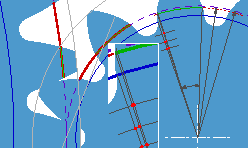
\includegraphics[width=1.0\textwidth]{part2/ruote/FIG/ruote/1160c_ix.pdf}
\begin{picture}(0,0)(200,0)
\scriptsize{
\color{white}
\put(270,40){$z_1=11$}
\put(40,120){$z_2=60$}
\put(270,18){$O_1$}
\put(39,28){$r_{b_2}$}
\put(96,78){$r_{{p_2}_f}$}
\put(182,185){$l_1$}
\put(98,140){$l_2$}
\put(167,178){$\mu$}
\put(258,187){$\zeta$}
\put(262,175){$\gamma(\theta_0)$}
\put(264,165){$\gamma(\theta_f)$}
\put(217,83){$\zeta$}
\put(220,54){$\gamma(\theta_0)$}
\put(227.5,27){$\gamma(\theta_f)$}
\put(291,106){$\delta_1$}
\color{black}
\put(232,185){$r_{b_1}$}
\put(120,210){$r_{t_2}$}
\put(97,167){$p$}
\put(162,219){$r_{t_1}$}
\put(147,149){$p$}
\put(354.5,189){$r_{{p_1}_f}$}
\put(329.5,199.5){$r_{{p_1}_0}$}
}
\end{picture}
\end{center}
\vskip -5mm
\caption{\em
Ingranaggio con $z_1=11$, $z_2=60$, $\theta_0=20^{\circ}$, $\theta_f=22^{\circ}$, $i_0=142$, $i_f=143.9$, con le correzioni $x_1=0.5$ e $x_2=0$.
} 
\vskip -3mm
\label{fig:1160c_ix}
\end{figure}
Esporremo per primo quello che porta 
all'individuazione dell'interasse
di funzionamento $i_f$ e del corrispondente angolo di pressione $\theta_f$,
date le due correzioni arbitrarie delle ruote. 
Il secondo caso fa invece riferimento
all'individuazione di quelle correzioni necessarie a produrre un interasse
di funzionamento dato.
Riprendiamo dalla figura \ref{fig:1160c_ix} e cerchiamo di individuare
un criterio, date le correzioni delle due ruote, per potere stabilire
l'effettivo interasse di funzionamento e l'effettivo angolo di pressione.
Da un punto di vista cinematico, l'ingranaggio della figura appena citata
funzionerebbe egregiamente anche con l'interasse dato dalla somma dei
raggi delle primitive teoriche pi\`u la somma delle correzioni:
$i_g=(z_1 +z_2) m /2 +(x_1+x_2)m$. Se montassimo in questo modo le ruote,
noteremmo per\`o un certo gioco che, in generale, non pu\`o essere tollerato
nelle trasmissioni di potenza, onde evitare che i denti ``sbattano''
\index{sbattimento} a causa delle eventuali (frequentissime nelle varie
applicazioni) inversioni della direzione del flusso di
potenza. Ecco quindi il criterio cercato: le ruote devono essere montate senza gioco\footnote{
Un minimo gioco tra le ruote deve sempre sussistere, per evitare ai cuscinetti
di supporto di funzionare in regime di carico gravoso e non previsto,
ma soprattutto per consentire la lubrificazione dei denti. La 
quantificazione di tale gioco \`e una questione delicata che dipende da
un numero rilevante di fattori: condizione di impiego della coppia di ruote,
precisione e finitura 
delle ruote stesse, tipo di lubrificazione, e molti altri. Rimandiamo
gli studenti desiderosi di approfondire alla letteratura specializzata, 
come ad esempio \cite{henriot}.
}.
Riferendoci ancora alla figura \ref{fig:1160c_ix}, quanto appena stabilito
si traduce nella seguente relazione $p=l_1 + l_2$. Questa relazione afferma
che il passo sulle primitive di funzionamento $p$, il quale ovviamente,
affinch\'e le ruote possano ingranare, deve essere lo stesso
su entrambe, \`e dato dalla
somma dello spessore dei denti sulle primitive stesse.
\`E questo uno dei casi in cui scopriamo l'utilit\`a della rappresentazione
analitica dell'evolvente e, in particolare, della \ref{eq:gamma}.
Cominciamo col calcolare la lunghezza dell'arco della primitiva teorica, o
di riferimento,
che attraversa un dente. A questo proposito notiamo che, quando la dentiera viene
spostata della quantit\`a $c=mx$, il vano sulla primitiva di taglio, che sar\`a
pari allo spessore del dente sulla primitiva di riferimento della ruota, vale
\begin{equation}
l_0= m \left( \tfrac{\pi}{2} + 2 x \tan(\theta_0) \right)\,,
\label{eq:l0}
\end{equation}
\noindent dove l'addendo di destra non \`e altro che la base di un triangolo
isoscele di altezza pari a $c=mx$ e angolo di apertura uguale al 
doppio dell'angolo dei profili della dentiera. La \ref{eq:l0} va specializzata
per le due ruote, in quanto le correzioni $x_1$ e $x_2$ saranno,
in generale, 
diverse. La conoscenza di $l_{0_1}$ e $l_{0_2}$ ci fornisce con facilit\`a
il valore degli angoli sottesi da tali archi:
\begin{equation}
\delta_1 = l_{0_1}/r_{{p_1}_0}\;\;\; {\rm e} \;\;\;\;
\delta_2 = l_{0_2}/r_{{p_2}_0}\,.
\label{eq:delta}
\end{equation}
\noindent Le lunghezze degli archi $l_1$ e $l_2$ si otterranno considerando
gli effettivi valori del raggio primitivo di funzionamento delle due ruote 
e l'aumento degli angoli $\delta$ dovuti all'angolo $\zeta$, come riportato
in figura \ref{fig:1160c_ix}.
Quanto a $\zeta$, sempre dalla figura, abbiamo
\begin{equation}
\zeta= \gamma(\theta_0)-\gamma(\theta_f)\,,
\label{eq:zeta}
\end{equation}
\noindent e tale valore\footnote{
Per la coordinata polare dell'evolvente abbiamo mantenuto la nomenclatura
esposta nella formula \ref{eq:gamma}, $\gamma()$, bench\'e
il nome pi\`u comunemente usato nella letteratura sia {\em involute
function}\index{involute function}. Pertanto, con un'abbreviazione a nostro
parere infelice, abbiamo
\begin{equation}
 {\rm inv}(\theta) = \tan(\theta)-\theta \,,
\label{eq:inv}
\end{equation}
come si trova, ad esempio, in \cite{henriot}.
} sar\`a lo stesso per le due ruote. Finalmente ricaviamo
\begin{equation}
l_1= r_{{p_1}_f} (\delta_1-2\zeta)\;\;\; {\rm e} \;\;\; l_2= r_{{p_2}_f} (\delta_2-2\zeta)\,,
\label{eq:l1l2}
\end{equation}
\noindent quindi, per il passo $p=l_1+l_2$, misurato sulle primitive di 
funzionamento possiamo scrivere
\begin{multline}
p= l_1+l_2= 
2 r_{{p_1}_f}[ \frac{1}{z_1} (\pi/2 + 2 x_1 \tan(\theta_0)) + \zeta] +\\
+2 r_{{p_2}_f}[ \frac{1}{z_2} (\pi/2 + 2 x_2 \tan(\theta_0)) + \zeta]\,.
\end{multline} 
\noindent A valle di alcune semplici sostituzioni, tenendo presente 
che $r_{{p_1}_f}= z_1 p/\pi$ e $r_{{p_2}_f}= z_2 p/\pi$,
esplicitando $\zeta$ tramite la \ref{eq:zeta}, otteniamo
\begin{equation}
\gamma(\theta_f)=2 \frac{x_1+x_2}{z_1+z_2}\tan(\theta_0) +\gamma(\theta_0)\,.
\label{eq:thetaf}
\end{equation}
\noindent La funzione $\gamma(\theta)$, col nome citato nella \ref{eq:inv}, \`e
riportata, tabulata, in diversi trattati: citiamo \cite{henriot} dove,
dalla pagina 72 alla pagina 79, $\theta$ spazia da $10^{\circ}$ a $50^{\circ}$. Tale funzione \`e
regolare e monotona crescente, pertanto, senza scomodare metodi di ricerca
degli zeri recanti nomi altisonanti, il comune metodo di bisezione
(che abbiamo usato per ottenere le nostre figure) porta,
con estrema rapidit\`a, a soluzioni apprezzabili della \ref{eq:thetaf}. Una
volta individuato il valore di $\theta_f$, che sar\`a l'effettivo angolo di
pressione, ricordando che in ogni caso
il raggio della circonferenza di base non cambia,
come abbiamo gi\`a altrove sottolineato, avremo
\begin{equation}
r_{{p_1}_f} \cos(\theta_f)=r_{{p_1}_0} \cos(\theta_0)\;\;\; {\rm e} \;\;\;
r_{{p_2}_f} \cos(\theta_f)=r_{{p_2}_0} \cos(\theta_0)\,,
\end{equation}
\noindent dalle quali si ottiene
\begin{equation}
i_f= r_{{p_1}_f} + r_{{p_2}_f}=  (r_{{p_2}_0}+ r_{{p_1}_0}) \frac{ \cos(\theta_0)}{\cos(\theta_f)}= m(z_1+z_2)\frac{ \cos(\theta_0)}{2 \cos(\theta_f)}\,.
\label{eq:if}
\end{equation}
\begin{wrapfigure}{r}{0.54\textwidth}
      \begin{center}
      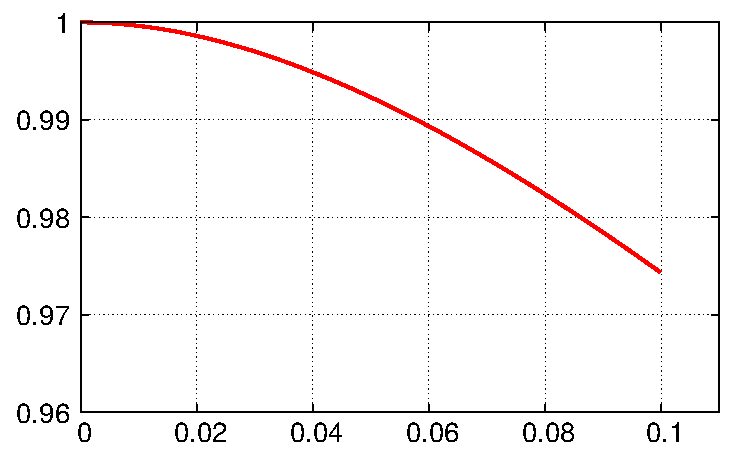
\includegraphics[width=0.52\textwidth]{part2/ruote/FIG/ruote/interasse.pdf}
     \end{center}
\begin{picture}(0,0)(-63,1)
\scriptsize{
        \put(-46,119){$\ni$}
        \put(78,19){$1-i_f/i_0$}
}
\end{picture}
\vskip -4.1mm
        \caption{\em Rapporto tra interasse effettivo $i_f$ e interasse
intuitivo $i_0+m(x_1+x_2)$.}
     \label{fig:interasse}
\end{wrapfigure}
\noindent Ci sembrano opportune le seguenti due considerazioni. La prima:
$\cos(\theta_f)$, e perci\`o anche l'interasse di funzionamento $i_f$, dipende
soltanto dalla somma delle correzioni quindi, come gi\`a ammesso nel
precedente paragrafo, se $x_1 + x_2=0$ risulta $\theta_f=\theta_0$ e $i_f=i_0$,
 cio\`e angolo di pressione e interasse rimangono inalterati.
 La seconda osservazione pu\`o essere elaborata
come risposta alla domanda: l'interasse di funzionamento sar\`a dato da
 $i_f=i_0+m(x_1+x_2)$? La risposta \`e no, e per convincerci di ci\`o
studiamo l'andamento del rapporto tra l'interasse effettivo e la somma delle
correzioni addizionata all'interasse teorico, che chiamiamo $\ni$
\begin{equation}
\ni=\frac{i_f}{i_0+m(x_1+x_2)}\,,
\label{eq:ni}
\end{equation}
\noindent in funzione
della variazione adimensionale dell'interasse $\delta_i=1-i_f/i_0$.
\noindent La figura \ref{fig:interasse} mostra quindi il grafico di $\ni$
al variare di $\delta_i$, che per $0<=\delta_i<=0.1$  
evidenzia una riduzione di $i_f$ rispetto
all'interasse che si sarebbe individuato a intuito $i_0+m(x_1+x_2)$.
Tale situazione dovr\`a, peraltro, risultare compatibile con i giochi tra testa e piede
 dei denti e richiede pertanto una specifica verifica.
\vskip 3mm
\noindent Veniamo ora al secondo dei due casi emblematici
per le correzioni con variazione di interasse, che \`e quello 
in cui le correzioni incognite devono
risultare compatibili con un interasse dato. Stabilito quindi il valore di $i_f$,
dalla \ref{eq:if} ricaviamo $\theta_f$, come gi\`a accennato con la 
formula \ref{eq:nuove_primitive}.
Dalla \ref{eq:thetaf} ricaviamo poi,
con facilit\`a, la somma delle correzioni $x_1+x_2$ ammissibile con 
l'interasse di funzionamento assegnato. 
Il tema della ripartizione delle
correzioni sulle due ruote \`e complesso e rientra nell'ambito dello
studio dei criteri di scelta delle correzioni stesse. Ribadiamo che
decidere di dare al pignone la minima correzione necessaria a scongiurare
il sottotaglio dei denti e quindi regolarci di conseguenza circa la correzione
della seconda ruota, magari con una correzione di segno opposto, cos\`i
da lasciare inalterato l'interasse di progetto,
 \`e molto riduttivo e anacronistico. 
Una guida alla scelta delle correzioni tramite percorsi volti
 all'ottimizzazione degli ingranaggi (percorsi e criteri
 a volte in contesa
tra loro) \`e riportata in \cite{righettini}. Riteniamo per\`o fuori
dallo scopo di queste note approfondire ulteriormente questo tema che,
come abbiamo anticipato, \`e materia decisamente specialistica.
\begin{figure}[hbt]
      \begin{center}
      
\includegraphics[width=0.65\textwidth]{part2/ruote/FIG/ruote/forma_dente.pdf}
     \end{center}
\begin{picture}(0,0)(-63,1)
\scriptsize{
\color{white}
        \put(30,53){$x=-0.3$}
        \put(37,65){$x=0$}
        \put(31,79){$x=0.3$}
        \put(31,93){$x=0.6$}
        \put(25,110){$x=1.086$}
}
\end{picture}
\vskip -5mm
        \caption{\em
Variazione della forma dei denti di una ruota con $z=17$ e correzioni $x=-0.3$, $x=0$, $x=0.3$, $x=0.6$ e $x=1.086$.
}
     \label{fig:forma_dente}
\end{figure}

\noindent Riepiloghiamo
l'argomento della correzione del profilo dei denti sottolineando tre punti
che ci sembrano importanti. 
Il primo riguarda la forma del dente, sensibilmente modificata
dallo spostamento del profilo,
come riportato in figura \ref{fig:forma_dente}.
Al crescere della correzione si passa infatti dalla condizione di
 sottotaglio a quella
che vede l'irrobustimento della 
base dei denti, fino all'appuntimento dei denti stessi quando si 
adottano valori di correzione eccessivi.
Nella figura \`e appunto riportato, per una ruota con $z=17$, il
caso di appuntimento del dente, quando le due evolventi si incrociano esattamente
sulla circonferenza di testa. La situazione dei denti a punta, ma anche con
spessore di testa troppo piccolo, \`e da evitarsi per ragioni di resistenza
meccanica.

\noindent Il secondo punto saliente riguarda
 il fattore di ricoprimento $f_c$. Esso, in sostanza, dipende
dalla somma delle correzioni $x_1 + x_2$, e 
diminuisce al crescere di questa somma, mentre non \`e molto sensibile ai valori
delle singole correzioni.
Con $x_1+x_2=0$, il fattore di ricoprimento \`e compreso tra $1.4<f_c<2$, che
ovviamente \`e anche l'intervallo dove spazia tale fattore per le ruote
non corrette.
Adottando correzioni la cui somma \`e negativa si possono
ottenere elevati valori del fattore di ricoprimento, a beneficio della
silenziosit\`a dell'ingranaggio.
Quando invece $x_1 + x_2 > 0$ il fattore di ricoprimento diminuisce e questo
pu\`o arrivare a compromettere
 la continuit\`a della trasmissione. Pertanto, nel caso di correzioni a
somma algebrica maggiore di zero, cio\`e con aumento dell'interasse,
bisogna sempre verificare il valore di $f_c$.

\noindent Il terzo punto riguarda l'allontanamento del segmento dei
 contatti $AB$ dalle ruote con correzione positiva. Ridurre la porzione
di accesso sulla linea dei contatti porta un netto
miglioramento del rendimento degli ingranaggi. Per tale motivo ai pignoni
motori, che sono una buona parte di quelli che si costruiscono, si applicano
volentieri correzioni positive che, eliminando il sottotaglio e irrobustendo
la base del dente a favore della sua resistenza strutturale, ne migliorano anche
il rendimento diminuendo il tratto di accesso, come mostra il confronto
tra i tratti $PA$ e $PB$ della figura \ref{fig:1160c_i0}.
Le cose vanno diversamente per i moltiplicatori di velocit\`a, dove la ruota
motrice non necessiterebbe, di per s\'e, correzioni positive con lo scopo
di eliminare il sosttotaglio. In tali casi, i diagrammi che ci guidano
nel ripartire la somma delle correzioni $x_1+x_2$ sulle due ruote possono
allocare una correzione positiva maggiore alla ruota motrice, cio\`e,
in questo caso, quella con maggiore numero di denti, come mostrato
in \cite{righettini}, pag. 52, e, in alcuni casi, persino 
tollerare un leggero
sottotaglio sulla ruota condotta, quella cio\`e con numero di denti minore.

\section{Note Conclusive sulle Ruote Dentate}

A conclusione di questo lungo capitolo, proponiamo un'analisi
ad elevatissima
 velocit\`a del percorso che, altrove, abbiamo seguito con la giusta
cadenza in modo da poter essere sviluppato senza incertezze. Tale traccia
ci ha condotto, quasi attraverso alcuni passaggi obbligati, alle ruote
con denti profilati a evolvente che dominano
interamente il panorama degli ingranaggi. Ad esempio, anche se non
ne abbiamo fatto cenno esplicito in questo lavoro, le ruote con denti ad asse
elicoidale, cio\`e le {\em ruote elicoidali}\index{ruote!elicoidali},
 pur possedendo caratteristiche specifiche, che un tecnico
deve conoscere perfettamente per poterle inserire correttamente 
nel progetto di una macchina, non
presentano, dal punto di vista della loro cinematica, nulla di diverso
dalle ruote che abbiamo studiato. Anzi, la loro fabbricazione si ottiene
semplicemente inclinando di un certo angolo l'utensile {\em Maag} di cui abbiamo
parlato diffusamente (oppure l'asse della ruota da tagliare).
Quindi profilo a evolvente ovunque, sulle ruote
coniche, che possono trasmettere il moto tra alberi concorrenti, sulle dentature
interne, e cos\`i via. Tale profilo si ottiene ``automaticamente'', come abbiamo visto,
dal processo di inviluppo tramite il taglio con utensili molto semplici.
In pratica, l'utilizzo dell'utensile pi\`u semplice da realizzare e da
affilare, cio\`e della dentiera riportata in figura
\ref{fig:dentiera_maag},
 ci fornisce direttamente e senza sforzo le ruote dentate a evolvente,
assortibili, facilmente adattabili a modeste variazioni di interasse,
facili da correggere per il raggiungimento di determinati scopi, come
l'eliminazione del sottotaglio dei denti.

\noindent E questa \`e
la conclusione alla quale ci premeva arrivare. Il successo di una 
tecnologia \`e spesso legato alla sua semplicit\`a e
alla sua attuabilit\`a.
Per questo tipo di  ruote non ha gran senso neppure lo studio numerico
del loro profilo come invece risulta d'obbligo,
da quando i calcolatori sono entrati a far parte degli strumenti
del progettista,  nella profilatura 
delle camme. Infatti, come abbiamo ormai troppe volte ripetuto,
l'ottenimento del loro sofisticato profilo
segue un processo
indiretto rappresentato dall'inviluppo creato dall'utensile dentiera,
processo che abbiamo usato anche noi per le nostre figure.
Anni fa, soprattutto
in fase prototipale, alcune
ruote dentate si lavoravano mediante l'impiego di frese a disco
che, scavando nel cilindro grezzo della futura ruota dentata
il vuoto tra un dente e il successivo,
modellavano i fianchi dei denti stessi.
Pu\`o darsi che qualche meccanico affezionato
alla {\em fresatura di forma}\index{fresatura di forma}
dei denti si possa ancora trovare presso
le officine che eseguono riparazioni e restauro di oggetti particolari.
La forma delle frese impiegate in questo procedimento
dipende naturalmente dal modulo della dentatura che si desidera ottenere,
ma anche, come \`e ovvio, dal numero dei denti della ruota.
Anzi, a ben vedere, sarebbe necessario impiegare 
una fresa per ogni ben preciso numero di denti.
Nella pratica per\`o bastano una decina di
utensili (di un certo modulo) per avere risultati soddisfacenti con
$z$ che spazia in un largo intervallo. Tagliando in
questo modo  il profilo dei denti
si perde per\`o completamente il controllo circa la 
capacit\`a della dentatura ottenuta di ospitare correttamente i denti
dell'altra ruota. \`E qui infatti che nasceva il problema dell'interferenza
propriamente detta,
la quale invece si manifesta come sottotaglio
dei denti quando questi si ottengono da un inviluppo. Rispetto alla
fresatura di forma,
il processo di taglio con creatore o dentiera {\em Maag} \`e
talmente pi\`u comodo, pi\`u preciso, pi\`u flessibile (si pensi
alle correzioni) da avere dato, dopo la sua comparsa,
una propulsione violenta a questo settore e allo sviluppo
della meccanica dello scorso secolo. Ma
cosa ci riserva il futuro? Si potrebbe pensare di fabbricare le ruote
dentate tagliandone direttamente il profilo con macchine
a controllo numerico, come potrebbe fare un'elettroerosione a filo?
Oppure, si potrebbe concepire di ottenerle tramite deposizione controllata
di materiale?  \`E chiaro che se si considerano queste opportunit\`a,
l'ottenimento dell'evolvente non \`e automatico e dovremmo
basarci su opportuni codici di calcolo che ci forniscano la geometria del
dente stesso. Su questo campo da gioco, poco conosciuto,
sospettiamo per\`o che il profilo a evolvente
avrebbe pi\`u di un concorrente.

\endinput
